% ============================================================
% BÁO CÁO ĐỒ ÁN TỐT NGHIỆP
% Hệ thống bãi đỗ xe tự động ứng dụng nhận diện biển số
% Biên dịch bằng: xelatex (bắt buộc, cần font Times New Roman)
% Lệnh biên dịch: xelatex bao_cao_do_an.tex (chạy 2 lần)
% ============================================================
\documentclass[a4paper,14pt]{extreport}

% --- Encoding & Font ---
\usepackage{fontspec}
\usepackage[vietnamese]{babel}
\setmainfont{Times New Roman}

% --- Page layout ---
\usepackage[top=2cm, bottom=2cm, left=3cm, right=2cm]{geometry}
\usepackage{setspace}
\setstretch{1.3}


% --- Graphics & Color ---
\usepackage{graphicx}
\usepackage{microtype}
\graphicspath{{hinh_latex/}}
\usepackage[dvipsnames,svgnames,x11names]{xcolor}
\usepackage{tikz}
\usetikzlibrary{shapes.geometric, arrows.meta, positioning, fit, backgrounds, calc}

% --- Tables ---
\usepackage{booktabs}
\usepackage{array}
\usepackage{longtable}
\usepackage{multirow}
\usepackage{tabularx}

% --- Listings (code) ---
\usepackage{listings}
\lstset{
  basicstyle=\ttfamily\small,
  breaklines=true,
  frame=single,
  backgroundcolor=\color{gray!10},
  xleftmargin=1em,
}

% --- Captions ---
\usepackage[font=small, labelfont=bf]{caption}
\usepackage{subcaption}

% --- Hyperlinks ---
\usepackage{hyperref}
\hypersetup{
  colorlinks=true,
  linkcolor=NavyBlue,
  citecolor=OliveGreen,
  urlcolor=RoyalBlue,
}

% --- Header/Footer ---
\usepackage{fancyhdr}
\pagestyle{fancy}
\fancyhf{}
\fancyhead[R]{\small\leftmark}
\fancyfoot[C]{\thepage}
\renewcommand{\headrulewidth}{0.4pt}

% --- Float placement ---
\usepackage{float}

% --- Enumeration ---
\usepackage{enumitem}
\setlist[itemize]{label={--}, leftmargin=2em}

% --- TikZ styles ---
\tikzstyle{block} = [rectangle, rounded corners, minimum width=2.5cm, minimum height=1cm, align=center, inner sep=2mm, draw=black, fill=blue!8, font=\small]
\tikzstyle{decision} = [diamond, aspect=2.5, minimum width=2cm, align=center, inner sep=1mm, draw=black, fill=yellow!15, font=\small]
\tikzstyle{arrow} = [thick, ->, >=Stealth]
\tikzstyle{darrow} = [thick, <->, >=Stealth]
\tikzstyle{process} = [rectangle, minimum width=2cm, minimum height=0.8cm, align=center, inner sep=2mm, draw=black, fill=green!8, font=\small]
\tikzstyle{reject} = [rectangle, rounded corners, minimum width=2cm, minimum height=0.8cm, align=center, inner sep=2mm, draw=red!70, fill=red!8, font=\small]
\tikzstyle{accept} = [rectangle, rounded corners, minimum width=2cm, minimum height=0.8cm, align=center, inner sep=2mm, draw=green!70!black, fill=green!12, font=\small]


% ============================================================
\begin{document}

% --- Title Page ---
\begin{titlepage}
\centering
\vspace*{1cm}
{\Large\bfseries TRƯỜNG ĐẠI HỌC GIAO THÔNG VẬN TẢI}\\[0.2cm]
{\large\bfseries KHOA ĐIỆN - ĐIỆN TỬ}\\[0.2cm]
{\large\bfseries BỘ MÔN KỸ THUẬT VIỄN THÔNG}\\[2cm]

\rule{\textwidth}{1.5pt}\\[0.5cm]
{\LARGE\bfseries BÁO CÁO ĐỀ TÀI TỐT NGHIỆP}\\[0.4cm]
{\Large\bfseries \underline{\textit{Đề tài:}} HỆ THỐNG KIỂM SOÁT PHƯƠNG TIỆN RA VÀO\\[0.2cm] ỨNG DỤNG XỬ LÝ ẢNH}\\[0.5cm]
\rule{\textwidth}{1.5pt}\\[2cm]

\begin{flushleft}
\hspace{2.5cm}{\large\bfseries Sinh viên thực hiện} \hspace{0.5cm} {\large : \textbf{LÊ SÔNG THAO}}\\[0.3cm]
\hspace{2.5cm}{\large\bfseries Lớp - Khóa} \hspace{1.8cm} {\large : \textbf{Kỹ thuật Điện tử Tin học Công nghiệp 2 - K62}}\\[0.3cm]
\hspace{2.5cm}{\large\bfseries Giảng viên hướng dẫn} \hspace{0.05cm} {\large : \textbf{TS. Nguyễn Thúy Bình}}\\
\end{flushleft}

\vfill
{\large\bfseries \textit{Hà Nội 2026}}
\end{titlepage}

% --- Table of Contents ---
\tableofcontents
\newpage
\listoffigures
\newpage
\listoftables
\newpage


% ============================================================
% TÓM TẮT
% ============================================================
\chapter*{TÓM TẮT}
\addcontentsline{toc}{chapter}{TÓM TẮT}

Báo cáo trình bày quá trình thiết kế và xây dựng mô hình hệ thống bãi đỗ xe tự động ứng dụng nhận diện biển số. Hệ thống sử dụng hai camera cho cổng vào và cổng ra, mô hình YOLOv8 để phát hiện vùng biển số, PaddleOCR để nhận dạng ký tự, thuật toán hậu xử lý theo định dạng biển số Việt Nam để chọn kết quả cuối, SQLite để quản lý dữ liệu và Arduino để điều khiển hai servo barrier thông qua tín hiệu cảm biến LM393.

Nội dung báo cáo được trình bày theo hướng từ tổng quát đến chi tiết: trước hết xác định bài toán và sơ đồ khối tổng quan, sau đó phân tích cơ sở lý thuyết của từng khối, tiếp theo là thiết kế hệ thống theo luồng dữ liệu và luồng điều khiển, cuối cùng đánh giá kết quả thực nghiệm. Trọng tâm kỹ thuật của đề tài là khối nhận diện biển số và khối điều khiển phần cứng barrier an toàn.


% ============================================================
% DANH MỤC TỪ VIẾT TẮT
% ============================================================
\chapter*{DANH MỤC TỪ VIẾT TẮT}
\addcontentsline{toc}{chapter}{DANH MỤC TỪ VIẾT TẮT}

\begin{longtable}{>{\bfseries}l p{5cm} p{6cm}}
\toprule
\textbf{Thuật ngữ} & \textbf{Viết đầy đủ} & \textbf{Nghĩa sử dụng} \\
\midrule
\endfirsthead
\toprule
\textbf{Thuật ngữ} & \textbf{Viết đầy đủ} & \textbf{Nghĩa sử dụng} \\
\midrule
\endhead
AI & Artificial Intelligence & Trí tuệ nhân tạo \\
CLAHE & Contrast Limited Adaptive Histogram Equalization & Cân bằng lược đồ xám thích nghi \\
COM & Communication Port & Cổng giao tiếp nối tiếp \\
CPU & Central Processing Unit & Bộ xử lý trung tâm \\
GPU & Graphics Processing Unit & Bộ xử lý đồ họa \\
GND & Ground & Chân mass/đất chung \\
IoU & Intersection over Union & Tỷ lệ giao/hợp giữa hai hộp \\
mAP & mean Average Precision & Độ chính xác trung bình \\
OCR & Optical Character Recognition & Nhận dạng ký tự quang học \\
PWM & Pulse Width Modulation & Điều chế độ rộng xung \\
SQLite & Structured Query Language Lite & Hệ cơ sở dữ liệu nhúng \\
USB & Universal Serial Bus & Chuẩn kết nối máy tính \\
VCC & Voltage Common Collector & Chân cấp nguồn dương \\
YOLO & You Only Look Once & Mô hình phát hiện đối tượng \\
YOLOv8 & YOLO version 8 & Phiên bản 8 của YOLO \\
\bottomrule
\end{longtable}


% ============================================================
% CHƯƠNG 1
% ============================================================
\chapter{TỔNG QUAN ĐỀ TÀI}

\section{Đặt vấn đề}

Trong các bãi đỗ xe truyền thống, việc kiểm soát phương tiện thường được thực hiện thủ công thông qua nhân viên bảo vệ, vé giấy hoặc ghi chép bằng tay. Cách làm này có một số hạn chế như tốn nhân lực, dễ nhầm lẫn khi ghi nhận biển số, khó kiểm tra lịch sử vào ra và chưa đảm bảo tính tự động trong quá trình vận hành.

Với sự phát triển của xử lý ảnh, trí tuệ nhân tạo và vi điều khiển, việc xây dựng một hệ thống bãi đỗ xe tự động có khả năng nhận diện biển số, quản lý dữ liệu và điều khiển barrier (thanh chắn/barie) là hướng tiếp cận phù hợp cho các mô hình bãi xe thông minh. Hệ thống có thể tự động ghi nhận biển số phương tiện, kiểm tra điều kiện cho phép vào hoặc ra, đồng thời điều khiển barrier (thanh chắn/barie) thông qua phần cứng.

Đề tài này tập trung xây dựng mô hình bãi đỗ xe tự động sử dụng camera (thiết bị thu hình) để thu nhận hình ảnh biển số, mô hình YOLOv8 (You Only Look Once version 8 - mô hình phát hiện đối tượng phiên bản 8) để phát hiện vùng biển số, PaddleOCR (Paddle Optical Character Recognition - bộ nhận dạng ký tự quang học) để nhận dạng ký tự, SQLite (Structured Query Language Lite - hệ cơ sở dữ liệu nhúng dạng file) để lưu trữ dữ liệu và Arduino (bo mạch vi điều khiển) để điều khiển servo (động cơ điều khiển theo góc quay) barrier (thanh chắn/barie) dựa trên tín hiệu cảm biến vật cản LM393 (module cảm biến vật cản dùng IC so sánh LM393).

\section{Mục tiêu đề tài}

Mục tiêu chính của đề tài là xây dựng một hệ thống mô phỏng bãi đỗ xe tự động có khả năng vận hành theo cả chế độ tự động và thủ công. Hệ thống cần đáp ứng các yêu cầu sau:

\begin{itemize}[leftmargin=2em]
  \item Thu nhận hình ảnh từ camera (thiết bị thu hình) cổng vào và camera (thiết bị thu hình) cổng ra.
  \item Nhận diện biển số xe từ ảnh chụp camera (thiết bị thu hình).
  \item Kiểm tra biển số với danh sách biển số hợp lệ.
  \item Quản lý danh sách xe đang có trong bãi.
  \item Kiểm tra số lượng chỗ trống trước khi cho xe vào.
  \item Kiểm tra xe có trong bãi trước khi cho xe ra.
  \item Điều khiển barrier (thanh chắn/barie) cổng vào và cổng ra bằng servo (động cơ điều khiển theo góc quay).
  \item Đọc tín hiệu cảm biến để xác định xe đang chắn barrier (thanh chắn/barie) hay đã đi qua.
  \item Đóng barrier (thanh chắn/barie) sau khi cảm biến không còn phát hiện vật cản trong một khoảng thời gian an toàn.
  \item Hiển thị trạng thái camera (thiết bị thu hình), biển số, số lượng xe, nhật ký và trạng thái phần cứng trên giao diện.
\end{itemize}

\section{Phạm vi thực hiện}

Đề tài được thực hiện ở mức mô hình đồ án, tập trung vào việc chứng minh nguyên lý hoạt động của một hệ thống bãi xe tự động. Phạm vi của hệ thống gồm:

\begin{itemize}[leftmargin=2em]
  \item Mô hình bãi xe quy mô nhỏ với số lượng chỗ giới hạn.
  \item Hai cổng hoạt động độc lập: cổng vào và cổng ra.
  \item Hai camera (thiết bị thu hình) tương ứng với hai cổng.
  \item Một mạch Arduino (bo mạch vi điều khiển) điều khiển hai servo (động cơ điều khiển theo góc quay) và đọc hai cảm biến LM393 (module cảm biến vật cản dùng IC so sánh LM393).
  \item Phần mềm điều khiển chạy trên máy tính bằng Python (ngôn ngữ lập trình Python).
  \item Cơ sở dữ liệu cục bộ dùng SQLite (hệ cơ sở dữ liệu nhúng dạng file).
  \item Nhận diện biển số trong điều kiện camera (thiết bị thu hình) được lắp đặt và căn chỉnh phù hợp.
\end{itemize}
Đề tài chưa mở rộng đến các chức năng thương mại như tính phí tự động, thanh toán điện tử, quản lý người dùng nhiều cấp hoặc triển khai trên hệ thống máy chủ từ xa.

\section{Bài toán tổng thể}

Bài toán của hệ thống có thể mô tả như sau: khi một phương tiện đi tới cổng vào hoặc cổng ra, cảm biến phát hiện vật cản và gửi trạng thái về máy tính thông qua Arduino (bo mạch vi điều khiển). Phần mềm lấy khung hình từ camera (thiết bị thu hình) tương ứng, nhận diện biển số xe, kiểm tra dữ liệu trong cơ sở dữ liệu rồi quyết định có mở barrier (thanh chắn/barie) hay không. Sau khi phương tiện đi qua, cảm biến không còn phát hiện xe, hệ thống chờ thêm một khoảng thời gian an toàn rồi hạ barrier (thanh chắn/barie).

Quy trình này cần đảm bảo ba yêu cầu quan trọng:

\begin{itemize}[leftmargin=2em]
  \item \textbf{Đúng dữ liệu:} biển số phải được nhận diện và đối chiếu chính xác.
  \item \textbf{Đúng logic vận hành:} xe vào, xe ra, bãi đầy, xe không hợp lệ phải được xử lý khác nhau.
  \item \textbf{An toàn cơ khí:} barrier (thanh chắn/barie) không được hạ ngay khi xe vẫn còn nằm trong vùng cảm biến.
\end{itemize}

\section{Sơ đồ khối tổng quan hệ thống}

\textbf{Hình 1.1} mô tả cấu trúc tổng quát của hệ thống. Hệ thống được chia thành sáu khối chính:

\begin{itemize}[leftmargin=2em]
  \item \textbf{Khối thu nhận hình ảnh:} gồm camera (thiết bị thu hình) cổng vào và camera (thiết bị thu hình) cổng ra, có nhiệm vụ cung cấp khung hình cho hệ thống xử lý.
  \item \textbf{Khối nhận diện biển số:} phát hiện vùng biển số, xử lý ảnh, nhận dạng ký tự và trả về chuỗi biển số.
  \item \textbf{Khối điều khiển trung tâm:} tiếp nhận dữ liệu từ camera (thiết bị thu hình), cảm biến, cơ sở dữ liệu và quyết định điều khiển barrier (thanh chắn/barie).
  \item \textbf{Khối cơ sở dữ liệu:} lưu danh sách biển số hợp lệ, xe trong bãi, sức chứa và lịch sử vào ra.
  \item \textbf{Khối giao diện người dùng:} hiển thị camera (thiết bị thu hình), kết quả nhận diện, trạng thái hệ thống và cho phép thao tác thủ công.
  \item \textbf{Khối phần cứng barrier (thanh chắn/barie):} gồm Arduino (bo mạch vi điều khiển), servo (động cơ điều khiển theo góc quay) và cảm biến LM393 (module cảm biến vật cản dùng IC so sánh LM393) để thực hiện đóng mở cổng.
\end{itemize}
\textbf{Hình 1.2} minh họa cách bố trí phần cứng trong mô hình. Mỗi cổng có một camera (thiết bị thu hình) để thu ảnh biển số, một cảm biến LM393 (module cảm biến vật cản dùng IC so sánh LM393) để phát hiện xe tại vùng barrier (thanh chắn/barie) và một servo (động cơ điều khiển theo góc quay) để nâng hạ thanh chắn. Camera (thiết bị thu hình) cần được đặt sao cho biển số nằm trọn trong khung hình, còn cảm biến cần nằm tại vùng xe đi qua để hỗ trợ cơ chế đóng barrier (thanh chắn/barie) an toàn.

\begin{figure}[H]
\centering
\begin{tikzpicture}[every node/.style={font=\small}]
  % Trung tâm
  \node[block, fill=orange!15, text width=3.8cm, minimum height=1.5cm] (dk) at (0,0) {\textbf{Khối điều khiển trung tâm}};
  
  % Trên
  \node[block, fill=cyan!15, text width=3.5cm] (cam) at (0, 3.5) {\textbf{Khối thu nhận hình ảnh}\\(Camera cổng vào/ra)};
  
  % Trái
  \node[block, fill=purple!15, text width=3.5cm] (ai) at (-5.8, 0) {\textbf{Khối nhận diện biển số}\\(YOLOv8 + PaddleOCR)};
  
  % Phải
  \node[block, fill=gray!15, text width=3.5cm] (ui) at (5.8, 0) {\textbf{Khối giao diện người dùng}\\(Hiển thị và Thao tác)};
  
  % Dưới Trái
  \node[block, fill=green!15, text width=3.5cm] (db) at (-3.5, -3.5) {\textbf{Khối cơ sở dữ liệu}\\(Lưu danh sách, lịch sử)};
  
  % Dưới Phải
  \node[block, fill=yellow!15, text width=3.5cm] (hw) at (3.5, -3.5) {\textbf{Khối phần cứng barrier}\\(Arduino, Servo, LM393)};

  % Mũi tên và text (Dùng sloped và align=center để tránh đè chữ lên khung)
  \draw[arrow] (cam) -- node[right, font=\scriptsize]{Khung hình} (dk);
  
  % Điều khiển <-> Nhận diện (2 mũi tên song song)
  \draw[arrow] (dk.170) -- node[above, font=\scriptsize, align=center]{Frame ảnh} (ai.10);
  \draw[arrow] (ai.350) -- node[below, font=\scriptsize, align=center]{Kết quả\\biển số} (dk.190);
  
  % Điều khiển <-> Giao diện
  \draw[darrow] (dk) -- node[above, font=\scriptsize, align=center]{Trạng thái /\\Thao tác} (ui);
  
  % Điều khiển <-> CSDL (sloped để chữ nằm nghiêng theo mũi tên)
  \draw[darrow] (dk) -- node[above, sloped, font=\scriptsize, align=center]{Truy vấn / Cập nhật} (db);
  
  % Điều khiển <-> Phần cứng
  \draw[darrow] (dk) -- node[above, sloped, font=\scriptsize, align=center]{Lệnh / Cảm biến} (hw);
\end{tikzpicture}
\caption{Sơ đồ khối tổng quan hệ thống}
\label{fig:tong_quan}
\end{figure}

\section{Ý nghĩa thực tiễn của đề tài}

Hệ thống giúp mô phỏng một quy trình quản lý bãi xe tự động có tính thực tế cao. Thay vì chỉ nhận diện biển số đơn lẻ, đề tài kết hợp cả phần mềm, cơ sở dữ liệu, giao diện và phần cứng điều khiển. Điều này giúp người thực hiện hiểu rõ mối liên hệ giữa xử lý ảnh, điều khiển tự động và quản lý dữ liệu trong một hệ thống nhúng kết hợp máy tính.

---

\chapter{CƠ SỞ LÝ THUYẾT}

\section{Tổng quan các khối lý thuyết}

Hệ thống bãi đỗ xe tự động trong đề tài được xây dựng từ nhiều khối kỹ thuật khác nhau. Các khối này không hoạt động riêng lẻ mà liên kết với nhau thành một chuỗi xử lý thống nhất:

1. Camera thu nhận hình ảnh phương tiện.
2. Mô hình nhận diện tìm vùng biển số.
3. Bộ OCR (Optical Character Recognition - nhận dạng ký tự quang học) đọc ký tự trên biển số.
4. Bộ hậu xử lý chuẩn hóa kết quả theo định dạng biển số Việt Nam.
5. Bộ điều khiển trung tâm kiểm tra dữ liệu và quyết định mở/đóng cổng.
6. Arduino (bo mạch vi điều khiển) thực hiện điều khiển servo (động cơ điều khiển theo góc quay) và gửi trạng thái cảm biến.
7. Cơ sở dữ liệu lưu trữ trạng thái bãi xe.
8. Giao diện hiển thị và cho phép người dùng điều khiển.

\section{Khối nhận diện biển số}

Khối nhận diện biển số là khối kỹ thuật trọng tâm của hệ thống, đóng vai trò quyết định dữ liệu đầu vào cho toàn bộ quá trình quản lý xe. Thay vì chỉ dùng một mô hình OCR đơn giản, hệ thống thiết kế một luồng xử lý (pipeline) phức tạp và chặt chẽ gồm nhiều bước nối tiếp nhau nhằm đảm bảo độ chính xác cao nhất trong nhiều điều kiện môi trường. Quá trình này được thực hiện tuần tự qua 6 bước như sau:

\textbf{Bước 1: Tiếp nhận nguồn ảnh đầu vào}
\begin{itemize}[leftmargin=2em]
  \item \textbf{Nguồn ảnh:} Lấy trực tiếp từ luồng video (stream) của camera cổng vào hoặc cổng ra.
  \item \textbf{Định dạng:} Mỗi khung hình (frame) được trích xuất là một ma trận điểm ảnh (numpy array) ở hệ màu BGR (định dạng chuẩn của OpenCV).
  \item \textbf{Mục tiêu:} Cung cấp khung hình toàn cảnh chứa phương tiện và biển số cho hệ thống phân tích.
\end{itemize}
\textbf{Bước 2: Phát hiện và cắt vùng biển số (YOLOv8)}
\begin{itemize}[leftmargin=2em]
  \item \textbf{Mô hình và Cấu hình:} Sử dụng mô hình YOLOv8n (bản nano nhẹ và nhanh). Trọng số mô hình \texttt{bien\_so\_yolo.pt} đã được huấn luyện trước trên tập dữ liệu biển số Việt Nam (100 epochs, kích thước ảnh 640x640, batch 16).
  \item \textbf{Thông số dự đoán:} Hàm nhận diện chạy với độ tin cậy tối thiểu \texttt{conf=0.25}, kích thước xử lý \texttt{imgsz=640} và chạy trên môi trường \texttt{CPU}.
  \item \textbf{Kết quả xử lý:} YOLO trả về tọa độ hộp giới hạn (bounding box - \texttt{x1, y1, x2, y2}) của các vùng nghi ngờ là biển số.
  \item \textbf{Cắt ảnh (Crop):} Hệ thống dùng tọa độ này để cắt (crop) riêng vùng biển số ra khỏi ảnh toàn cảnh. Việc cắt nhỏ ảnh giúp OCR chạy nhanh hơn và không bị nhiễu bởi các chữ viết xuất hiện trên phông nền (như chữ trên áo, biển quảng cáo).
\end{itemize}
*Hình 2.1. Chuỗi xử lý (pipeline) nhận diện biển số từ ảnh camera.*

\textbf{Bước 3: Tiền xử lý - Tạo các phiên bản ảnh (OpenCV)}
\begin{itemize}[leftmargin=2em]
  \item \textbf{Số lượng ảnh sinh ra:} Từ 1 ảnh crop vùng biển số ban đầu, hệ thống tạo ra 3 phiên bản ảnh khác nhau để tối đa hóa khả năng đọc của OCR trong mọi điều kiện ánh sáng.
  \item \textbf{Môi trường:} Xử lý bằng thư viện OpenCV.
  \item \textbf{Các phiên bản:}
\end{itemize}
  1. \textbf{Ảnh gốc (BGR):} Giữ lại màu sắc tự nhiên, hoạt động tốt khi điều kiện ánh sáng lý tưởng.
  2. \textbf{Ảnh CLAHE:} Ảnh được chuyển sang ảnh xám (grayscale) và áp dụng thuật toán CLAHE (Contrast Limited Adaptive Histogram Equalization) với thông số \texttt{clipLimit=2.0}, \texttt{tileGridSize=(8, 8)}. Phương pháp này giúp cân bằng sáng, làm rõ nét chữ khi biển số bị lóa đèn hoặc nằm trong vùng sấp bóng.
  3. \textbf{Ảnh Otsu:} Lấy ảnh CLAHE đi qua bộ lọc \texttt{cv2.threshold} với cờ \texttt{THRESH\_BINARY + THRESH\_OTSU} để phân ngưỡng tự động. Chữ và nền được tách biệt hoàn toàn thành 2 màu Đen/Trắng, vô cùng hiệu quả với ảnh có độ tương phản cao.

\textbf{Bước 4: Nhận dạng ký tự quang học (PaddleOCR)}
\begin{itemize}[leftmargin=2em]
  \item \textbf{Môi trường:} Sử dụng mô hình PaddleOCR mã nguồn mở.
  \item \textbf{Quá trình thực thi:} 3 phiên bản ảnh (Gốc, CLAHE, Otsu) được lần lượt đưa vào PaddleOCR một cách độc lập.
  \item \textbf{Ghép dòng tạo ứng viên:} Với các biển số xe máy gồm 2 dòng, PaddleOCR thường nhận diện thành nhiều mảnh rời rạc. Hệ thống sẽ thu thập toàn bộ các dòng chữ đọc được, ghép nối chúng lại thành một chuỗi văn bản hoàn chỉnh. Tập hợp chuỗi được ghép và các mảnh rời này tạo thành một danh sách các "ứng viên" (candidates) tiềm năng.
\end{itemize}
*Hình 2.3. Chi tiết quá trình sinh 3 phiên bản ảnh, qua OCR và chấm điểm.*

\textbf{Bước 5: Chuẩn hóa và Sửa lỗi theo vị trí (Post-processing)}
Hậu xử lý là bắt buộc vì mô hình OCR tổng quát không hiểu luật biển số Việt Nam và thường nhầm lẫn giữa số và chữ (VD: 0 và O, 1 và I, 5 và S).
\begin{itemize}[leftmargin=2em]
  \item \textbf{Chuẩn hóa:} Dùng Biểu thức chính quy (Regex) \texttt{[^A-Za-z0-9]} để loại bỏ hoàn toàn các ký tự lạ, dấu gạch ngang, dấu chấm, khoảng trắng, và chuyển toàn bộ chuỗi về chữ in hoa.
  \item \textbf{Sửa lỗi theo vị trí:} Hệ thống rà soát chuỗi ký tự theo luật biển số VN. Ví dụ:
  \item 2 ký tự đầu tiên (mã tỉnh) bắt buộc phải là số. Nếu OCR đọc ra chữ \texttt{O}, \texttt{I}, \texttt{S}, \texttt{Z}, hệ thống tự động ép kiểu về \texttt{0}, \texttt{1}, \texttt{5}, \texttt{2}.
  \item Ký tự thứ 3 (seri) bắt buộc là chữ. Nếu OCR ra số \texttt{0}, \texttt{8}, hệ thống ép về chữ \texttt{D}, \texttt{B}.
\end{itemize}
\textbf{Bước 6: Chấm điểm và Lựa chọn kết quả cuối cùng}
\begin{itemize}[leftmargin=2em]
  \item \textbf{Quy tắc chấm điểm:} Mỗi ứng viên (sau khi chuẩn hóa) được chấm điểm dựa trên 3 yếu tố:
\end{itemize}
  1. *Khớp định dạng (Regex):* Chấm 1.0 điểm (hoàn hảo) nếu khớp định dạng Ô tô (2 số + 1 chữ + 5 số), Xe máy (2 số + 1 chữ + 6 số) hoặc Biển đặc biệt (2 số + 2 chữ + 5 số). Chấm 0.9 điểm nếu khớp một phần.
  2. *Độ tin cậy OCR:* Cộng thêm điểm trung bình độ tin cậy (Confidence score) mà PaddleOCR trả về.
  3. *Độ dài phù hợp:* Cộng điểm thưởng nhỏ (0.01 - 0.04) nếu độ dài chuỗi là 8 hoặc 9 ký tự (chuẩn độ dài biển số VN).
\begin{itemize}[leftmargin=2em]
  \item \textbf{Kết quả:} Hệ thống so sánh điểm số của tất cả các ứng viên sinh ra từ cả 3 nhánh ảnh. Ứng viên có tổng điểm cao nhất sẽ được chọn làm kết quả chuỗi biển số đầu ra để ghi vào Cơ sở dữ liệu. Đồng thời, hệ thống tạo ra một ảnh hiển thị phụ (nền đen chữ trắng) của biển số để hiển thị trực quan lên giao diện người dùng.
\end{itemize}

\begin{figure}[H]
\centering
\resizebox{0.95\textwidth}{!}{%
\begin{tikzpicture}[node distance=0.8cm and 0.8cm, every node/.style={font=\small}]
  % Hàng 1
  \node[block, fill=pink!20, text width=4cm] (crop) {\textbf{Vùng biển số}\\sau crop};
  
  % Hàng 2 (chia 3 nhánh ảnh)
  \node[block, fill=orange!10, text width=3cm, below=1cm of crop] (clahe) {\textbf{Ảnh CLAHE}};
  \node[block, fill=green!10, text width=3cm, left=0.5cm of clahe] (goc) {\textbf{Ảnh gốc}};
  \node[block, fill=gray!20, text width=3cm, right=0.5cm of clahe] (otsu) {\textbf{Ảnh Otsu}};
  
  % Hàng 3 (3 khối PaddleOCR)
  \node[block, fill=purple!10, text width=3cm, below=0.8cm of goc] (ocr_goc) {\textbf{PaddleOCR}};
  \node[block, fill=purple!10, text width=3cm, below=0.8cm of clahe] (ocr_clahe) {\textbf{PaddleOCR}};
  \node[block, fill=purple!10, text width=3cm, below=0.8cm of otsu] (ocr_otsu) {\textbf{PaddleOCR}};

  % Hàng 4 (Gộp lại)
  \node[block, fill=blue!10, text width=4cm, below=1.2cm of ocr_clahe] (ghep) {\textbf{Ghép dòng}\\tạo ứng viên};
  
  % Hàng 5
  \node[block, fill=blue!10, text width=4cm, below=0.8cm of ghep] (chuanhoa) {\textbf{Chuẩn hóa}\\Loại ký tự lạ\\Viết hoa};
  
  % Hàng 6
  \node[block, fill=blue!10, text width=4.5cm, below=0.8cm of chuanhoa] (sualoi) {\textbf{Sửa lỗi theo vị trí}\\O $\rightarrow$ 0, I $\rightarrow$ 1, S $\rightarrow$ 5\\tại vị trí cần số};

  % Hàng 7
  \node[block, fill=yellow!15, text width=4.5cm, below=0.8cm of sualoi] (chamdiem) {\textbf{Chấm điểm}\\$\bullet$ Confidence OCR\\$\bullet$ Khớp định dạng VN\\$\bullet$ Độ dài phù hợp};
  
  % Hàng 8
  \node[accept, text width=4.5cm, below=0.8cm of chamdiem] (kq) {\textbf{Biển số}\\có điểm cao nhất};
  
  % Mũi tên từ Crop -> 3 Ảnh
  \draw[arrow] (crop.south) -- ++(0,-0.4) -| (goc.north);
  \draw[arrow] (crop.south) -- (clahe.north);
  \draw[arrow] (crop.south) -- ++(0,-0.4) -| (otsu.north);
  
  % Mũi tên từ 3 Ảnh -> 3 OCR
  \draw[arrow] (goc.south) -- (ocr_goc.north);
  \draw[arrow] (clahe.south) -- (ocr_clahe.north);
  \draw[arrow] (otsu.south) -- (ocr_otsu.north);
  
  % Mũi tên từ 3 OCR -> Ghép dòng
  \draw[arrow] (ocr_goc.south) |- ++(0,-0.6) -| (ghep.north);
  \draw[arrow] (ocr_clahe.south) -- (ghep.north);
  \draw[arrow] (ocr_otsu.south) |- ++(0,-0.6) -| (ghep.north);
  
  % Mũi tên dọc
  \draw[arrow] (ghep.south) -- (chuanhoa.north);
  \draw[arrow] (chuanhoa.south) -- (sualoi.north);
  \draw[arrow] (sualoi.south) -- (chamdiem.north);
  \draw[arrow] (chamdiem.south) -- (kq.north);
\end{tikzpicture}
}%  end resizebox
\caption{Pipeline nhận diện biển số}
\label{fig:pipeline}
\end{figure}

\begin{figure}[H]
\centering
\resizebox{\textwidth}{!}{%
\begin{tikzpicture}[node distance=1.2cm and 1.2cm, every node/.style={font=\small}]
  % Hàng 1 (Trái sang phải)
  \node[block, fill=cyan!15, text width=3.2cm] (b1) {\textbf{Thu thập dữ liệu}\\hình ảnh};
  \node[block, fill=cyan!15, text width=3.2cm, right=of b1] (b2) {\textbf{Gán nhãn vùng}\\cần phát hiện};
  \node[block, fill=cyan!15, text width=3.2cm, right=of b2] (b3) {\textbf{Chia tập dữ liệu}\\(Train/Val/Test)};
  \node[block, fill=purple!12, text width=3.2cm, right=of b3] (b4) {\textbf{Khởi tạo}\\mô hình YOLOv8};
  
  % Hàng 2 (Phải sang trái)
  \node[block, fill=green!15, text width=3.2cm, below=1.5cm of b4] (b5) {\textbf{Tiến hành}\\huấn luyện};
  \node[block, fill=orange!15, text width=3.2cm, left=of b5] (b6) {\textbf{Đánh giá}\\kết quả mô hình};
  \node[accept, text width=3.2cm, left=of b6] (b7) {\textbf{Lựa chọn}\\mô hình tốt nhất};
  \node[block, fill=gray!15, text width=3.2cm, left=of b7] (b8) {\textbf{Trích xuất}\\để triển khai};
  
  % Mũi tên hàng 1
  \draw[arrow] (b1) -- (b2);
  \draw[arrow] (b2) -- (b3);
  \draw[arrow] (b3) -- (b4);
  
  % Mũi tên nối 2 hàng
  \draw[arrow] (b4) -- (b5);
  
  % Mũi tên hàng 2
  \draw[arrow] (b5) -- (b6);
  \draw[arrow] (b6) -- (b7);
  \draw[arrow] (b7) -- (b8);
\end{tikzpicture}
}
\caption{Quy trình huấn luyện YOLOv8 phát hiện biển số}
\label{fig:train_yolo}
\end{figure}

\section{Khối điều khiển tự động}

Khối điều khiển trung tâm hoạt động dựa trên sự kiện. Các sự kiện chính gồm:

\begin{itemize}[leftmargin=2em]
  \item Cảm biến cổng vào phát hiện xe.
  \item Cảm biến cổng ra phát hiện xe.
  \item AI (Artificial Intelligence - trí tuệ nhân tạo) trả về kết quả biển số.
  \item Người dùng bấm nút điều khiển thủ công.
  \item Camera bật/tắt hoặc mất khung hình.
  \item Arduino (bo mạch vi điều khiển) gửi trạng thái cảm biến.
\end{itemize}
Khi nhận được sự kiện, bộ điều khiển không xử lý độc lập từng sự kiện mà phải xét trạng thái hiện tại của toàn hệ thống. Ví dụ, nếu cảm biến cổng vào phát hiện xe nhưng bãi đã đầy thì không được mở barrier (thanh chắn/barie). Nếu xe ở cổng ra nhưng biển số không tồn tại trong danh sách xe đang ở trong bãi thì cũng không được mở cổng ra.

Điểm quan trọng của khối điều khiển là nó giữ vai trò ra quyết định, không để camera (thiết bị thu hình), AI (trí tuệ nhân tạo) hoặc Arduino (bo mạch vi điều khiển) tự mở cổng. Camera (thiết bị thu hình) chỉ cung cấp ảnh, AI (trí tuệ nhân tạo) chỉ trả về biển số, Arduino (bo mạch vi điều khiển) chỉ thực thi lệnh phần cứng. Quyết định cuối cùng như cho vào, từ chối, cho ra hoặc giữ barrier (thanh chắn/barie) mở đều nằm ở bộ điều khiển trung tâm.


\textbf{Hình 2.4} mô tả logic đóng barrier (thanh chắn/barie) an toàn. Các mũi tên thể hiện luồng kiểm tra lặp lại: nếu cảm biến còn phát hiện xe thì barrier (thanh chắn/barie) tiếp tục giữ mở; nếu cảm biến đã quang và duy trì đủ 2 giây thì hệ thống mới gửi lệnh đóng.

Barrier (thanh chắn/barie) không được đóng ngay khi có lệnh đóng nếu cảm biến vẫn đang phát hiện vật cản. Cơ chế an toàn được thiết kế như sau:

1. Khi barrier (thanh chắn/barie) đang mở, hệ thống theo dõi cảm biến tương ứng.
2. Nếu cảm biến còn phát hiện xe, hệ thống giữ barrier (thanh chắn/barie) ở trạng thái mở.
3. Khi cảm biến không còn phát hiện xe, hệ thống bắt đầu đếm thời gian.
4. Sau 2 giây không có vật cản, hệ thống mới gửi lệnh đóng barrier (thanh chắn/barie).

Cơ chế này giúp mô hình vận hành thực tế hơn, tránh trường hợp barrier (thanh chắn/barie) hạ quá sớm khi xe chưa đi qua hoàn toàn.

\begin{figure}[H]
\centering
\begin{tikzpicture}[node distance=1cm, every node/.style={font=\small}]
  \node[accept] (a) {Barrier đang MỞ};
  \node[decision, below=1cm of a] (b) {Cảm biến\\còn phát hiện xe?};
  \node[block, fill=orange!15, right=2cm of b] (c) {Giữ barrier MỞ};
  \node[decision, below=1.2cm of b] (e) {Xe đã từng\\chắn cảm biến?};
  \node[reject, right=2cm of e] (f) {Đóng barrier ngay};
  \node[block, below=1.2cm of e] (g) {Bắt đầu đếm\\thời gian quang};
  \node[decision, below=1cm of g] (h) {Đã đủ 2s?};
  \node[reject, below=1cm of h] (j) {Đóng barrier\\+ Cập nhật DB};
  
  \draw[arrow] (a) -- (b);
  \draw[arrow] (b) -- node[above]{Có} (c);
  \draw[arrow] (c) |- ([yshift=0.5cm]b.north) -- (b);
  \draw[arrow] (b) -- node[left]{Không} (e);
  \draw[arrow] (e) -- node[above]{Chưa} (f);
  \draw[arrow] (e) -- node[left]{Đã từng} (g);
  \draw[arrow] (g) -- (h);
  \draw[arrow] (h) -- node[left]{Đủ 2s} (j);
  \draw[arrow] (h.east) -- ++(1.5,0) node[above, font=\scriptsize]{Chưa} |- (b);
\end{tikzpicture}
\caption{Cơ chế an toàn khi đóng barrier}
\label{fig:dong_barrier}
\end{figure}

\section{Khối phần cứng và giao tiếp}

Arduino (bo mạch vi điều khiển) đóng vai trò là bộ điều khiển phần cứng. Trong đề tài, Arduino nhận lệnh từ máy tính qua Serial (giao tiếp nối tiếp), điều khiển hai servo (động cơ điều khiển theo góc quay) và đọc trạng thái hai cảm biến LM393 (module cảm biến vật cản dùng IC so sánh LM393).

Arduino (bo mạch vi điều khiển) giúp tách phần điều khiển cơ khí khỏi phần mềm máy tính. Máy tính chỉ cần gửi lệnh mức cao như mở cổng vào hoặc đóng cổng ra, còn Arduino thực hiện điều khiển servo (động cơ điều khiển theo góc quay) ở mức tín hiệu.

Servo (động cơ điều khiển theo góc quay) là động cơ có khả năng quay đến một góc xác định. Trong mô hình, servo được dùng để nâng và hạ thanh barrier (thanh chắn/barie). Hệ thống quy ước:

\begin{itemize}[leftmargin=2em]
  \item Góc đóng: barrier (thanh chắn/barie) nằm ngang, không cho xe qua.
  \item Góc mở: barrier (thanh chắn/barie) nâng lên, cho xe đi qua.
\end{itemize}
Để chuyển động thực tế hơn, servo (động cơ điều khiển theo góc quay) không quay tức thời từ góc đóng sang góc mở, mà được điều khiển từng bước nhỏ với độ trễ giữa các bước.

Cảm biến LM393 (module cảm biến vật cản dùng IC so sánh LM393) được dùng để phát hiện vật cản tại cổng vào và cổng ra. Khi có xe chắn vùng cảm biến, tín hiệu đầu ra thay đổi. Arduino (bo mạch vi điều khiển) đọc tín hiệu này và gửi trạng thái về máy tính.

Trong hệ thống, cảm biến không chỉ dùng để phát hiện xe xuất hiện mà còn dùng để quyết định thời điểm an toàn để đóng barrier (thanh chắn/barie).


\textbf{Hình 2.5} mô tả giao thức truyền nhận giữa máy tính và Arduino (bo mạch vi điều khiển). Mũi tên từ máy tính sang Arduino là luồng lệnh điều khiển; mũi tên từ Arduino về máy tính là luồng phản hồi trạng thái cảm biến và thông tin kiểm tra kết nối.

Máy tính và Arduino (bo mạch vi điều khiển) giao tiếp thông qua cổng Serial (giao tiếp nối tiếp). Giao thức được thiết kế đơn giản bằng chuỗi văn bản, giúp dễ kiểm tra bằng Serial Monitor (cửa sổ giám sát giao tiếp nối tiếp) và dễ mở rộng.

Một số lệnh từ máy tính gửi xuống Arduino (bo mạch vi điều khiển) được trình bày trong Bảng 2.1.

\textbf{Bảng 2.1. Giao thức lệnh gửi từ máy tính xuống Arduino (bo mạch vi điều khiển)}

Dữ liệu Arduino (bo mạch vi điều khiển) gửi lên máy tính có dạng:

``\texttt{text
CAM\_BIEN:xe\_vao=1,xe\_ra=0
}`\texttt{

Trong đó }xe_vao\texttt{ và }xe_ra\texttt{ thể hiện trạng thái cảm biến tại hai cổng.

Kênh Serial (giao tiếp nối tiếp) là hai chiều. Chiều từ máy tính xuống Arduino (bo mạch vi điều khiển) là lệnh điều khiển như mở hoặc đóng barrier (thanh chắn/barie). Chiều từ Arduino lên máy tính là trạng thái cảm biến và thông tin phản hồi. Việc dùng chuỗi văn bản làm giao thức giúp quá trình kiểm tra khi ghép nối phần cứng trở nên đơn giản: có thể mở Serial Monitor (cửa sổ giám sát giao tiếp nối tiếp) để gửi thử }SERVO_TEST\texttt{, }PING\texttt{ hoặc quan sát dòng }CAM_BIEN`.

\begin{table}[H]
\centering
\caption{Giao thức lệnh gửi từ máy tính xuống Arduino}
\label{tab:giao_thuc}
\begin{tabular}{ll}
\toprule
\textbf{Lệnh} & \textbf{Ý nghĩa} \\
\midrule
\texttt{VAO\_MO} & Mở barrier cổng vào \\
\texttt{VAO\_DONG} & Đóng barrier cổng vào \\
\texttt{RA\_MO} & Mở barrier cổng ra \\
\texttt{RA\_DONG} & Đóng barrier cổng ra \\
\texttt{PING} & Kiểm tra phản hồi Arduino \\
\texttt{SERVO\_TEST} & Kiểm tra hoạt động servo \\
\bottomrule
\end{tabular}
\end{table}

\section{Khối lưu trữ dữ liệu}

\textbf{Hình 2.6} mô tả các nhóm dữ liệu chính trong hệ thống. Bảng \texttt{xe\_trong\_bai} thể hiện trạng thái hiện tại của bãi xe, còn bảng \texttt{lich\_su\_ra\_vao} lưu lại các sự kiện đã xảy ra để phục vụ theo dõi.

SQLite (Structured Query Language Lite - hệ cơ sở dữ liệu nhúng dạng file) được sử dụng vì phù hợp với mô hình cục bộ, không cần cài đặt máy chủ cơ sở dữ liệu riêng. Cơ sở dữ liệu gồm bốn nhóm dữ liệu chính:

\begin{itemize}[leftmargin=2em]
  \item \textbf{Cấu hình:} lưu sức chứa bãi xe.
  \item \textbf{Biển số hợp lệ:} lưu danh sách biển số được phép vào.
  \item \textbf{Xe trong bãi:} lưu các xe đang hiện diện trong bãi.
  \item \textbf{Lịch sử vào ra:} lưu nhật ký sự kiện phục vụ theo dõi và kiểm tra.
\end{itemize}
---

\begin{figure}[H]
\centering
\begin{tikzpicture}[every node/.style={font=\small}]
  \node[block, fill=blue!10, minimum width=4cm] (caidat) at (0,0) {\textbf{cai\_dat}\\khoa (PK) | gia\_tri};
  \node[block, fill=green!10, minimum width=4cm] (bshl) at (6,0) {\textbf{bien\_so\_hop\_le}\\bien\_so (PK) | chu\_xe | tao\_luc};
  \node[block, fill=orange!10, minimum width=4cm] (xtb) at (0,-2.5) {\textbf{xe\_trong\_bai}\\bien\_so (PK) | vao\_luc};
  \node[block, fill=purple!10, minimum width=4cm] (lsrv) at (6,-2.5) {\textbf{lich\_su\_ra\_vao}\\id (PK) | bien\_so | su\_kien | thoi\_gian};
  
  \draw[arrow, dashed] (bshl) -- node[right, font=\scriptsize]{1:N} (lsrv);
  \draw[arrow, dashed] (bshl) -- node[above, font=\scriptsize]{1:N} (xtb);
\end{tikzpicture}
\caption{Sơ đồ cơ sở dữ liệu}
\label{fig:erd}
\end{figure}

\chapter{THIẾT KẾ VÀ ĐÁNH GIÁ HỆ THỐNG}

\section{Môi trường thực nghiệm}

Hệ thống được thử nghiệm trên mô hình bãi xe quy mô nhỏ. Môi trường thực nghiệm gồm:

\begin{itemize}[leftmargin=2em]
  \item Máy tính chạy phần mềm Python (ngôn ngữ lập trình Python) với giao diện Tkinter (thư viện giao diện đồ họa của Python).
  \item Camera USB/Full HD (camera dùng cổng USB, độ phân giải Full HD) dùng cho cổng vào và cổng ra.
  \item Arduino (bo mạch vi điều khiển) kết nối với máy tính qua cổng USB (Universal Serial Bus - chuẩn kết nối giữa máy tính và thiết bị).
  \item Hai servo (động cơ điều khiển theo góc quay) dùng để đóng/mở barrier (thanh chắn/barie).
  \item Hai cảm biến LM393 (module cảm biến vật cản dùng IC so sánh LM393) dùng để phát hiện xe tại cổng vào và cổng ra.
  \item Cơ sở dữ liệu SQLite (hệ cơ sở dữ liệu nhúng dạng file) lưu cục bộ trên máy tính.
\end{itemize}
Camera được căn chỉnh sao cho biển số nằm trong vùng quan sát, hạn chế bị cắt mất mép và giảm ảnh hưởng của ánh sáng chói.

\section{Nguyên tắc thiết kế}

Hệ thống được thiết kế theo hướng chia thành các khối chức năng độc lập. Mỗi khối đảm nhiệm một vai trò cụ thể, giúp quá trình kiểm tra, bảo trì và mở rộng dễ dàng hơn. Cách chia khối cũng giúp báo cáo và mô hình hóa hệ thống rõ ràng hơn.

Các nguyên tắc thiết kế chính:

\begin{itemize}[leftmargin=2em]
  \item Tách biệt giao diện, xử lý logic, nhận diện biển số, lưu trữ dữ liệu và điều khiển phần cứng.
  \item Luồng camera (thiết bị thu hình) và luồng AI (Artificial Intelligence - trí tuệ nhân tạo) không làm treo giao diện.
  \item Mọi quyết định mở cổng đều phải đi qua bộ điều khiển trung tâm.
  \item Cơ sở dữ liệu là nguồn xác định trạng thái xe trong bãi.
  \item Barrier chỉ được đóng khi cảm biến xác nhận vùng cổng đã an toàn.
\end{itemize}

\section{Kiến trúc phần mềm tổng thể}

\textbf{Hình 3.1} cho thấy bộ điều khiển trung tâm là điểm phối hợp chính giữa giao diện, camera (thiết bị thu hình), AI (trí tuệ nhân tạo), cơ sở dữ liệu và Arduino (bo mạch vi điều khiển). Các module (khối chức năng phần mềm) không tự quyết định mở cổng mà gửi dữ liệu về bộ điều khiển để xử lý thống nhất.

Hệ thống phần mềm gồm các khối sau:

\begin{itemize}[leftmargin=2em]
  \item \textbf{Khối giao diện:} hiển thị thông tin và nhận thao tác người dùng.
  \item \textbf{Khối điều khiển trung tâm:} điều phối toàn bộ hoạt động của hệ thống.
  \item \textbf{Khối camera (thiết bị thu hình):} đọc hình ảnh từ camera (thiết bị thu hình) vào và camera ra.
  \item \textbf{Khối AI (Artificial Intelligence - trí tuệ nhân tạo) nhận diện:} xử lý ảnh và trả về biển số.
  \item \textbf{Khối cơ sở dữ liệu:} lưu trữ và truy vấn thông tin xe.
  \item \textbf{Khối giao tiếp Arduino (bo mạch vi điều khiển):} gửi lệnh và đọc trạng thái phần cứng.
\end{itemize}
Khối điều khiển trung tâm là nơi liên kết các khối còn lại. Camera (thiết bị thu hình), AI (trí tuệ nhân tạo), cơ sở dữ liệu và Arduino (bo mạch vi điều khiển) không tự quyết định mở barrier (thanh chắn/barie); mọi quyết định đều được đưa về khối điều khiển trung tâm để đảm bảo thống nhất logic.

\begin{figure}[H]
\centering
\begin{tikzpicture}[node distance=1.5cm, every node/.style={font=\small}]
  \node[block, fill=cyan!15, minimum width=3.5cm] (gui) {giao\_dien\_chinh.py\\Giao diện Tkinter};
  \node[block, fill=orange!15, minimum width=3.5cm, below=of gui] (ctrl) {dieu\_khien\_he\_thong.py\\Bộ điều khiển};
  \node[block, fill=purple!15, minimum width=3.5cm, below left=1.5cm and 1cm of ctrl] (ai) {nhan\_dien\_bien\_so.py\\YOLOv8 + PaddleOCR};
  \node[block, fill=green!15, minimum width=3.5cm, below=of ctrl] (db) {quan\_ly\_du\_lieu.py\\SQLite};
  \node[block, fill=yellow!15, minimum width=3.5cm, below right=1.5cm and 1cm of ctrl] (ard) {giao\_tiep\_arduino.py\\Serial};
  
  \draw[darrow] (gui) -- (ctrl);
  \draw[arrow] (ctrl) -- (ai);
  \draw[arrow] (ai) -- (ctrl);
  \draw[darrow] (ctrl) -- (db);
  \draw[darrow] (ctrl) -- (ard);
\end{tikzpicture}
\caption{Sơ đồ module phần mềm}
\label{fig:module}
\end{figure}

\section{Luồng dữ liệu trong hệ thống}

\textbf{Hình 3.2} mô tả hướng di chuyển của dữ liệu giữa các khối. Dữ liệu ảnh đi từ camera (thiết bị thu hình) đến bộ điều khiển và AI (trí tuệ nhân tạo); dữ liệu biển số đi ngược về bộ điều khiển để kiểm tra cơ sở dữ liệu; lệnh điều khiển đi từ bộ điều khiển xuống Arduino (bo mạch vi điều khiển).

Luồng dữ liệu chính của hệ thống gồm:

1. Camera gửi khung hình mới nhất cho bộ điều khiển.
2. Khi có yêu cầu nhận diện, bộ điều khiển lấy khung hình và gửi vào hàng đợi AI (trí tuệ nhân tạo).
3. Khối AI (trí tuệ nhân tạo) trả về biển số và ảnh biển số đã xử lý để hiển thị.
4. Bộ điều khiển kiểm tra biển số với cơ sở dữ liệu.
5. Nếu đủ điều kiện, bộ điều khiển gửi lệnh mở barrier (thanh chắn/barie) cho Arduino (bo mạch vi điều khiển).
6. Arduino (bo mạch vi điều khiển) điều khiển servo (động cơ điều khiển theo góc quay) và gửi trạng thái cảm biến về máy tính.
7. Giao diện cập nhật trạng thái, nhật ký và kết quả nhận diện.

Việc tổ chức luồng dữ liệu theo hướng này giúp hạn chế xung đột giữa các tác vụ có tốc độ khác nhau. Camera (thiết bị thu hình) cần cập nhật liên tục, AI (trí tuệ nhân tạo) xử lý chậm hơn, còn giao diện cần phản hồi ổn định cho người dùng.

\begin{figure}[H]
\centering
\begin{tikzpicture}[node distance=1cm, every node/.style={font=\small}]
  \node[block, fill=cyan!15] (cam) {Camera\\(luồng riêng)};
  \node[block, fill=orange!15, below=of cam] (dk) {Bộ điều khiển};
  \node[block, fill=purple!15, right=2cm of dk] (ai) {AI\\(luồng riêng)};
  \node[block, fill=green!15, below left=1.2cm and 0cm of dk] (db) {CSDL};
  \node[block, fill=yellow!15, below right=1.2cm and 0cm of dk] (ard) {Arduino};
  \node[block, fill=gray!15, below=2.8cm of dk] (ui) {Giao diện};
  
  \draw[arrow] (cam) -- node[left, font=\scriptsize]{1. Khung hình} (dk);
  \draw[arrow] (dk) -- node[above, font=\scriptsize]{3. Frame} (ai);
  \draw[arrow] (ai) -- node[below, font=\scriptsize]{4. Biển số} (dk);
  \draw[arrow] (dk) -- node[left, font=\scriptsize]{5. Kiểm tra} (db);
  \draw[arrow] (dk) -- node[right, font=\scriptsize]{7. Lệnh} (ard);
  \draw[arrow] (dk) -- node[left, font=\scriptsize]{9. Cập nhật} (ui);
\end{tikzpicture}
\caption{Luồng dữ liệu trong hệ thống}
\label{fig:luong_du_lieu}
\end{figure}

\section{Thiết kế khối nhận diện biển số}

Khối nhận diện biển số trong hệ thống được thiết kế như một dịch vụ xử lý ảnh độc lập. Đầu vào của khối là một frame (khung hình) BGR (Blue - Green - Red - thứ tự kênh màu xanh dương, xanh lá, đỏ trong OpenCV) lấy từ camera (thiết bị thu hình) cổng vào hoặc cổng ra. Đầu ra gồm hai phần: chuỗi biển số đã chuẩn hóa để bộ điều khiển kiểm tra logic, và ảnh biển số đã xử lý để hiển thị cho người dùng quan sát. Cách tách đầu ra như vậy giúp hệ thống vừa có dữ liệu dạng text (văn bản) để xử lý tự động, vừa có hình ảnh minh họa để người vận hành biết AI (trí tuệ nhân tạo) đang đọc từ vùng nào.

Khi bắt đầu chương trình, mô hình YOLO (You Only Look Once - mô hình phát hiện đối tượng một giai đoạn) và PaddleOCR (bộ nhận dạng ký tự quang học) được nạp vào bộ nhớ. Việc nạp mô hình thường tốn thời gian ở lần đầu, nên hệ thống có bước warm-up (chạy khởi động) để tránh trường hợp xe đầu tiên bị xử lý chậm bất thường. Khi cảm biến phát hiện xe, bộ điều khiển không gửi toàn bộ luồng video sang AI (trí tuệ nhân tạo), mà chỉ lấy frame (khung hình) mới nhất tại thời điểm cần nhận diện. Cách làm này giảm tải cho CPU (Central Processing Unit - bộ xử lý trung tâm)/GPU (Graphics Processing Unit - bộ xử lý đồ họa) và phù hợp với bài toán bãi xe: chỉ cần nhận diện khi có xe ở cổng, không cần OCR (nhận dạng ký tự quang học) liên tục 30 khung hình mỗi giây.

Ở bước phát hiện vùng biển, YOLO (mô hình phát hiện đối tượng một giai đoạn) trả về danh sách hộp giới hạn kèm độ tin cậy. Hệ thống chọn vùng biển số có điểm tin cậy phù hợp rồi crop (cắt vùng ảnh) từ ảnh gốc. Nếu crop quá sát, OCR (nhận dạng ký tự quang học) có thể mất một phần ký tự ở mép; nếu crop quá rộng, OCR dễ đọc nhiễu từ nền. Vì vậy trong mô hình thực tế, camera (thiết bị thu hình) cần được đặt sao cho biển số nằm đủ trong khung và kích thước biển số không quá lớn so với ảnh. Đây là lý do phần lắp đặt camera có ảnh hưởng trực tiếp đến độ chính xác nhận diện.

Sau khi có ảnh vùng biển số, hệ thống tạo ba phiên bản ảnh cho OCR (nhận dạng ký tự quang học). Ảnh gốc được giữ lại vì trong thực nghiệm đây là phiên bản cho độ chính xác rất cao khi ánh sáng ổn định. Ảnh CLAHE (cân bằng lược đồ xám thích nghi có giới hạn tương phản) được tạo bằng cách cân bằng tương phản cục bộ, giúp làm rõ nét chữ trong vùng sáng tối không đều. Ảnh Otsu (ảnh nhị phân theo ngưỡng Otsu) được tạo bằng cách nhị phân hóa, có tác dụng tách chữ và nền trong trường hợp biển số có độ tương phản mạnh. Ba ảnh này không nhằm làm đẹp giao diện, mà nhằm tạo nhiều điều kiện đọc khác nhau cho OCR.

Kết quả PaddleOCR (bộ nhận dạng ký tự quang học) có thể gồm nhiều dòng, đặc biệt với biển số xe máy hai dòng. Hệ thống tạo nhiều ứng viên từ kết quả OCR (nhận dạng ký tự quang học): chuỗi ghép tất cả các dòng và từng dòng riêng lẻ. Mỗi ứng viên được chuẩn hóa bằng cách loại bỏ ký tự không phải chữ/số, viết hoa và sửa lỗi theo vị trí. Sau đó hệ thống chấm điểm ứng viên theo ba yếu tố: độ tin cậy trung bình do OCR trả về, mức độ khớp với định dạng biển số Việt Nam và độ dài chuỗi phù hợp. Ứng viên có điểm cao nhất được chọn làm kết quả cuối.

Vai trò của từng bước trong khối nhận diện được tóm tắt trong Bảng 3.1.

\textbf{Bảng 3.1. Vai trò các bước trong khối nhận diện biển số}

Ảnh nền đen/chữ trắng được tạo sau cùng để hiển thị trực quan trên giao diện. Ảnh này giúp người dùng thấy rõ vùng ký tự mà hệ thống đang xử lý, nhưng không phải là dữ liệu duy nhất quyết định kết quả OCR (nhận dạng ký tự quang học). Quyết định nhận diện dựa trên nhiều ứng viên từ ảnh gốc, CLAHE (cân bằng lược đồ xám thích nghi có giới hạn tương phản) và Otsu (phương pháp tự động chọn ngưỡng nhị phân ảnh).

\begin{table}[H]
\centering
\caption{Vai trò các bước trong khối nhận diện biển số}
\label{tab:vai_tro_nhan_dien}
\begin{tabular}{p{3.5cm} p{4cm} p{5cm}}
\toprule
\textbf{Bước} & \textbf{Mục đích} & \textbf{Lý do cần thiết} \\
\midrule
YOLOv8 phát hiện & Tìm vùng biển số & Giảm nhiễu nền trước OCR \\
Crop vùng biển số & Tách vùng quan tâm & Tăng tốc và tăng độ chính xác \\
Tạo ảnh gốc/CLAHE/Otsu & Nhiều điều kiện đọc & Ánh sáng thay đổi \\
PaddleOCR & Đọc ký tự từ ảnh & Không cần train riêng \\
Chuẩn hóa chuỗi & Thống nhất text & Loại ký tự lạ \\
Sửa lỗi theo vị trí & Sửa nhầm chữ/số & Cấu trúc biển số VN \\
Chấm điểm & Chọn ứng viên tốt & Confidence + luật định dạng \\
\bottomrule
\end{tabular}
\end{table}

\section{Cấu hình huấn luyện YOLOv8}

Mô hình YOLOv8n được huấn luyện với các siêu tham số sau:

\begin{table}[H]
\centering
\caption{Cấu hình huấn luyện YOLOv8}
\label{tab:cau_hinh_train}
\begin{tabular}{lll}
\toprule
\textbf{Tham số} & \textbf{Giá trị} & \textbf{Ý nghĩa} \\
\midrule
Model & YOLOv8n & Biến thể nano, nhỏ gọn \\
Pretrained & yolov8n.pt & Trọng số khởi tạo sẵn \\
Epochs & 100 & Số vòng huấn luyện \\
Image size & 640 & Kích thước ảnh đầu vào \\
Batch size & 16 & Số ảnh mỗi lô \\
Optimizer & auto & Tự chọn tối ưu \\
lr0 & 0.01 & Learning rate khởi đầu \\
lrf & 0.01 & Learning rate cuối \\
Momentum & 0.937 & Hệ số quán tính SGD \\
Weight decay & 0.0005 & Hệ số phạt trọng số \\
Warmup epochs & 3.0 & Số epoch khởi động \\
Mosaic & 1.0 & Tăng cường ghép ảnh \\
Fliplr & 0.5 & Lật ngang 50\% \\
Scale & 0.5 & Thay đổi tỷ lệ \\
Close mosaic & 10 & Tắt mosaic 10 epoch cuối \\
AMP & true & Mixed precision training \\
Device & GPU (0) & Huấn luyện trên GPU \\
\bottomrule
\end{tabular}
\end{table}

\section{Kết quả huấn luyện YOLOv8}

\subsection{Chỉ số đánh giá chính}

\begin{table}[H]
\centering
\caption{Kết quả huấn luyện YOLOv8 (epoch 100)}
\label{tab:kq_yolo}
\begin{tabular}{lr}
\toprule
\textbf{Chỉ số} & \textbf{Kết quả} \\
\midrule
Precision & 99.18\% \\
Recall & 99.43\% \\
mAP50 & 99.48\% \\
mAP50-95 & 72.74\% \\
Train Box Loss (cuối) & 0.912 \\
Train Cls Loss (cuối) & 0.313 \\
Val Box Loss (cuối) & 1.017 \\
Val Cls Loss (cuối) & 0.323 \\
\bottomrule
\end{tabular}
\end{table}

\subsection{Biểu đồ quá trình huấn luyện}

\begin{figure}[H]
\centering
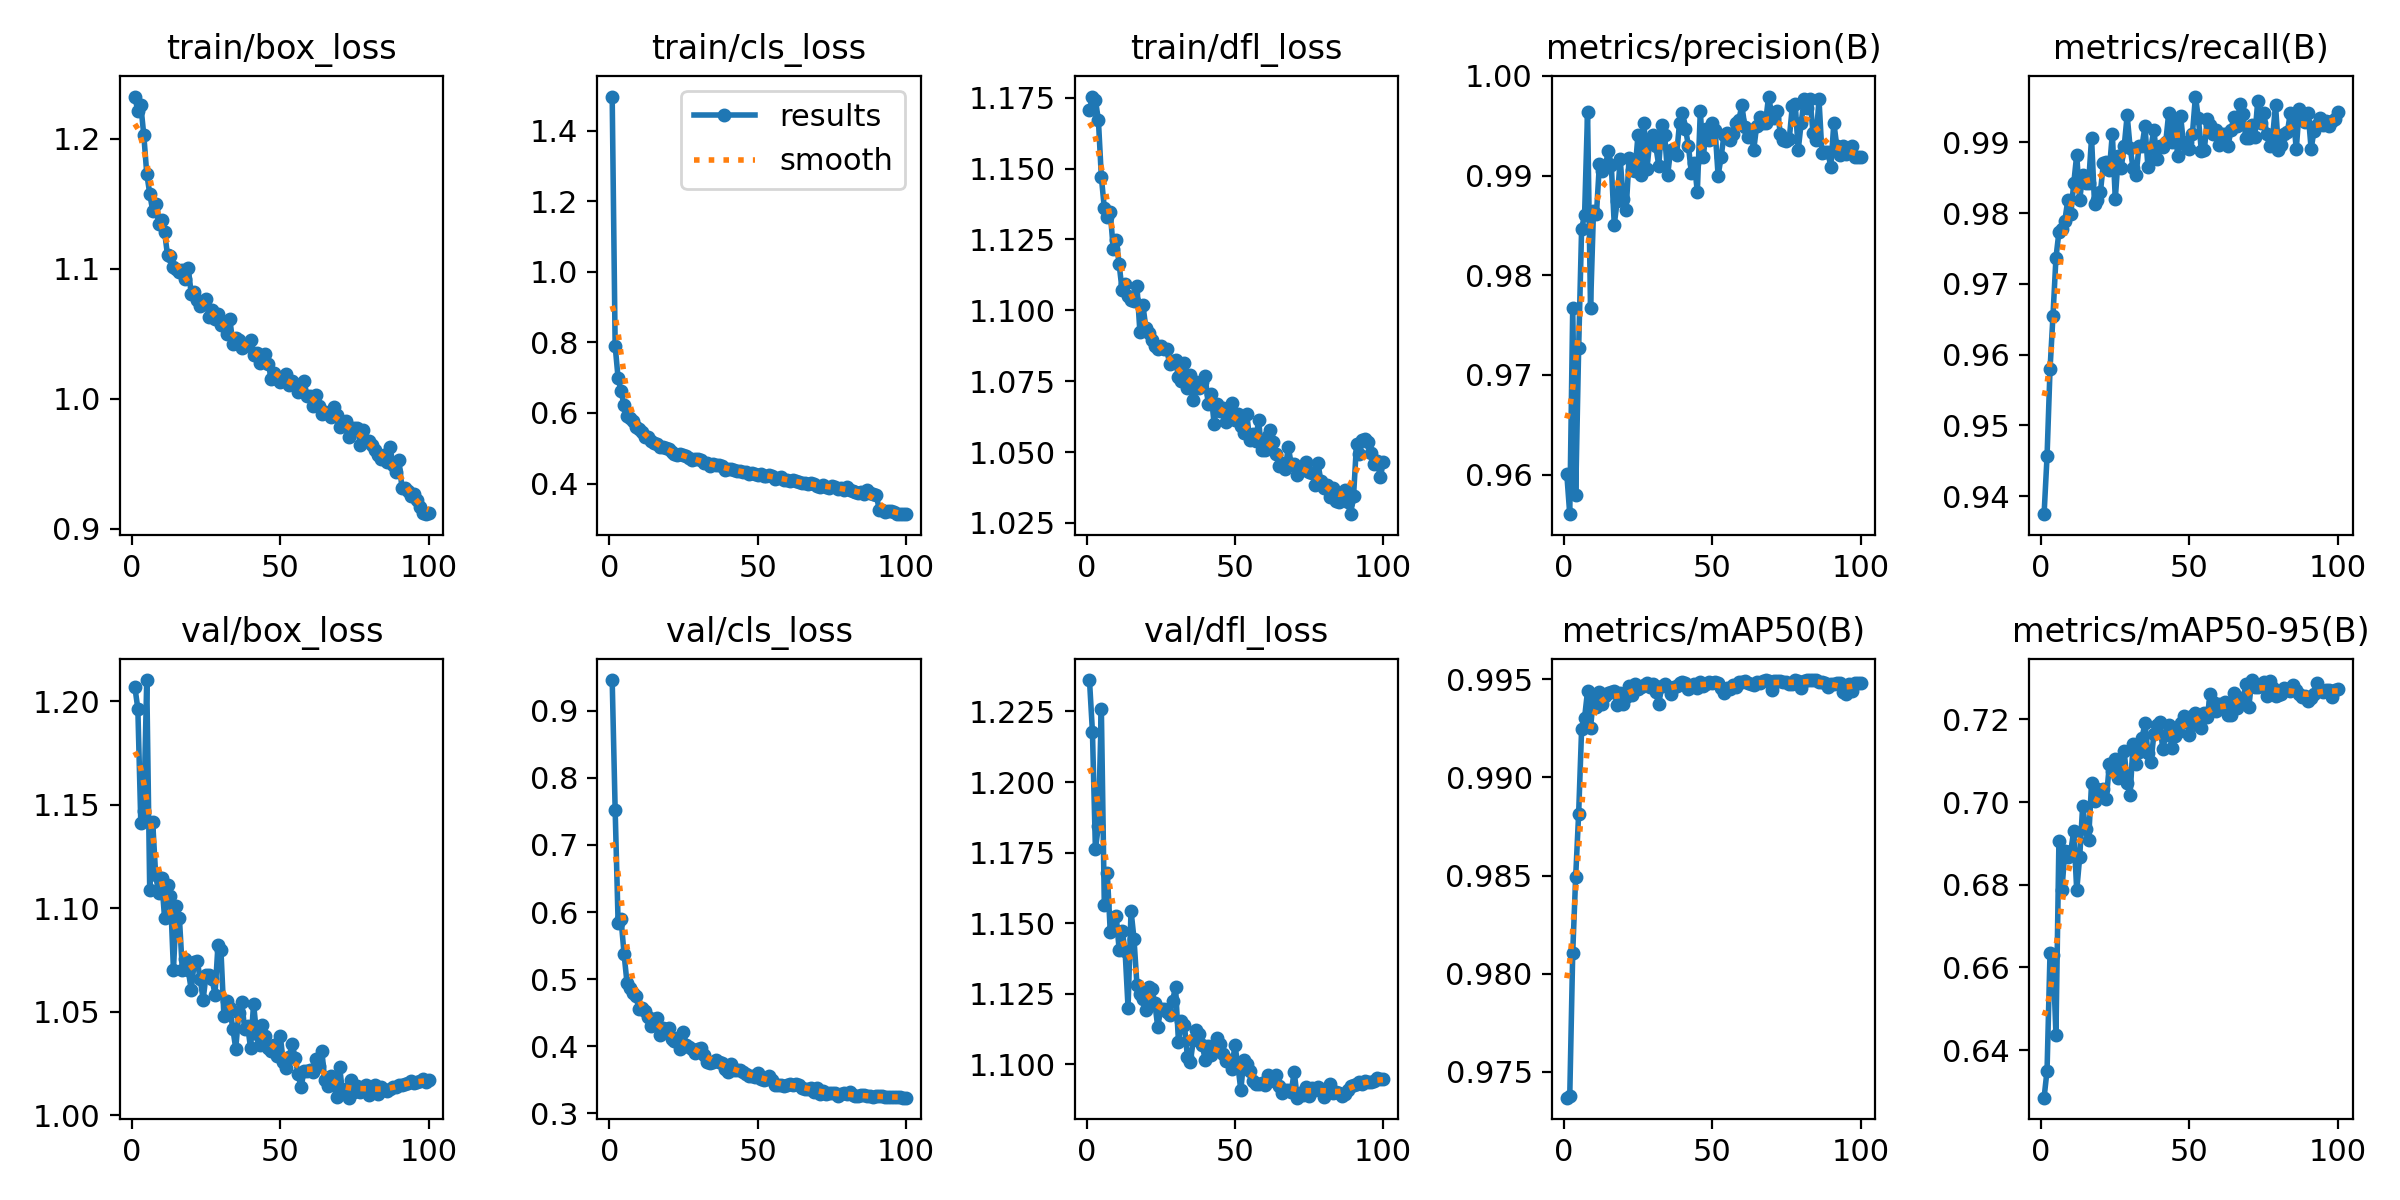
\includegraphics[width=0.85\textwidth]{results.png}
\caption{Biểu đồ tổng hợp quá trình huấn luyện YOLOv8 qua 100 epochs}
\label{fig:results}
\end{figure}

Nhận xét:
\begin{itemize}[leftmargin=2em]
  \item \textbf{Train loss} giảm đều đặn qua 100 epochs, mô hình học tốt và không bị overfitting.
  \item \textbf{Validation loss} ổn định từ epoch 50 trở đi, mô hình đã hội tụ.
  \item \textbf{Precision} và \textbf{Recall} đều đạt trên 99\% từ rất sớm.
  \item \textbf{mAP50} hội tụ nhanh đạt $\sim$99.48\%.
\end{itemize}

\subsection{Đường cong Precision, Recall, F1-Score}

\begin{figure}[H]
\centering
\begin{subfigure}[b]{0.48\textwidth}
  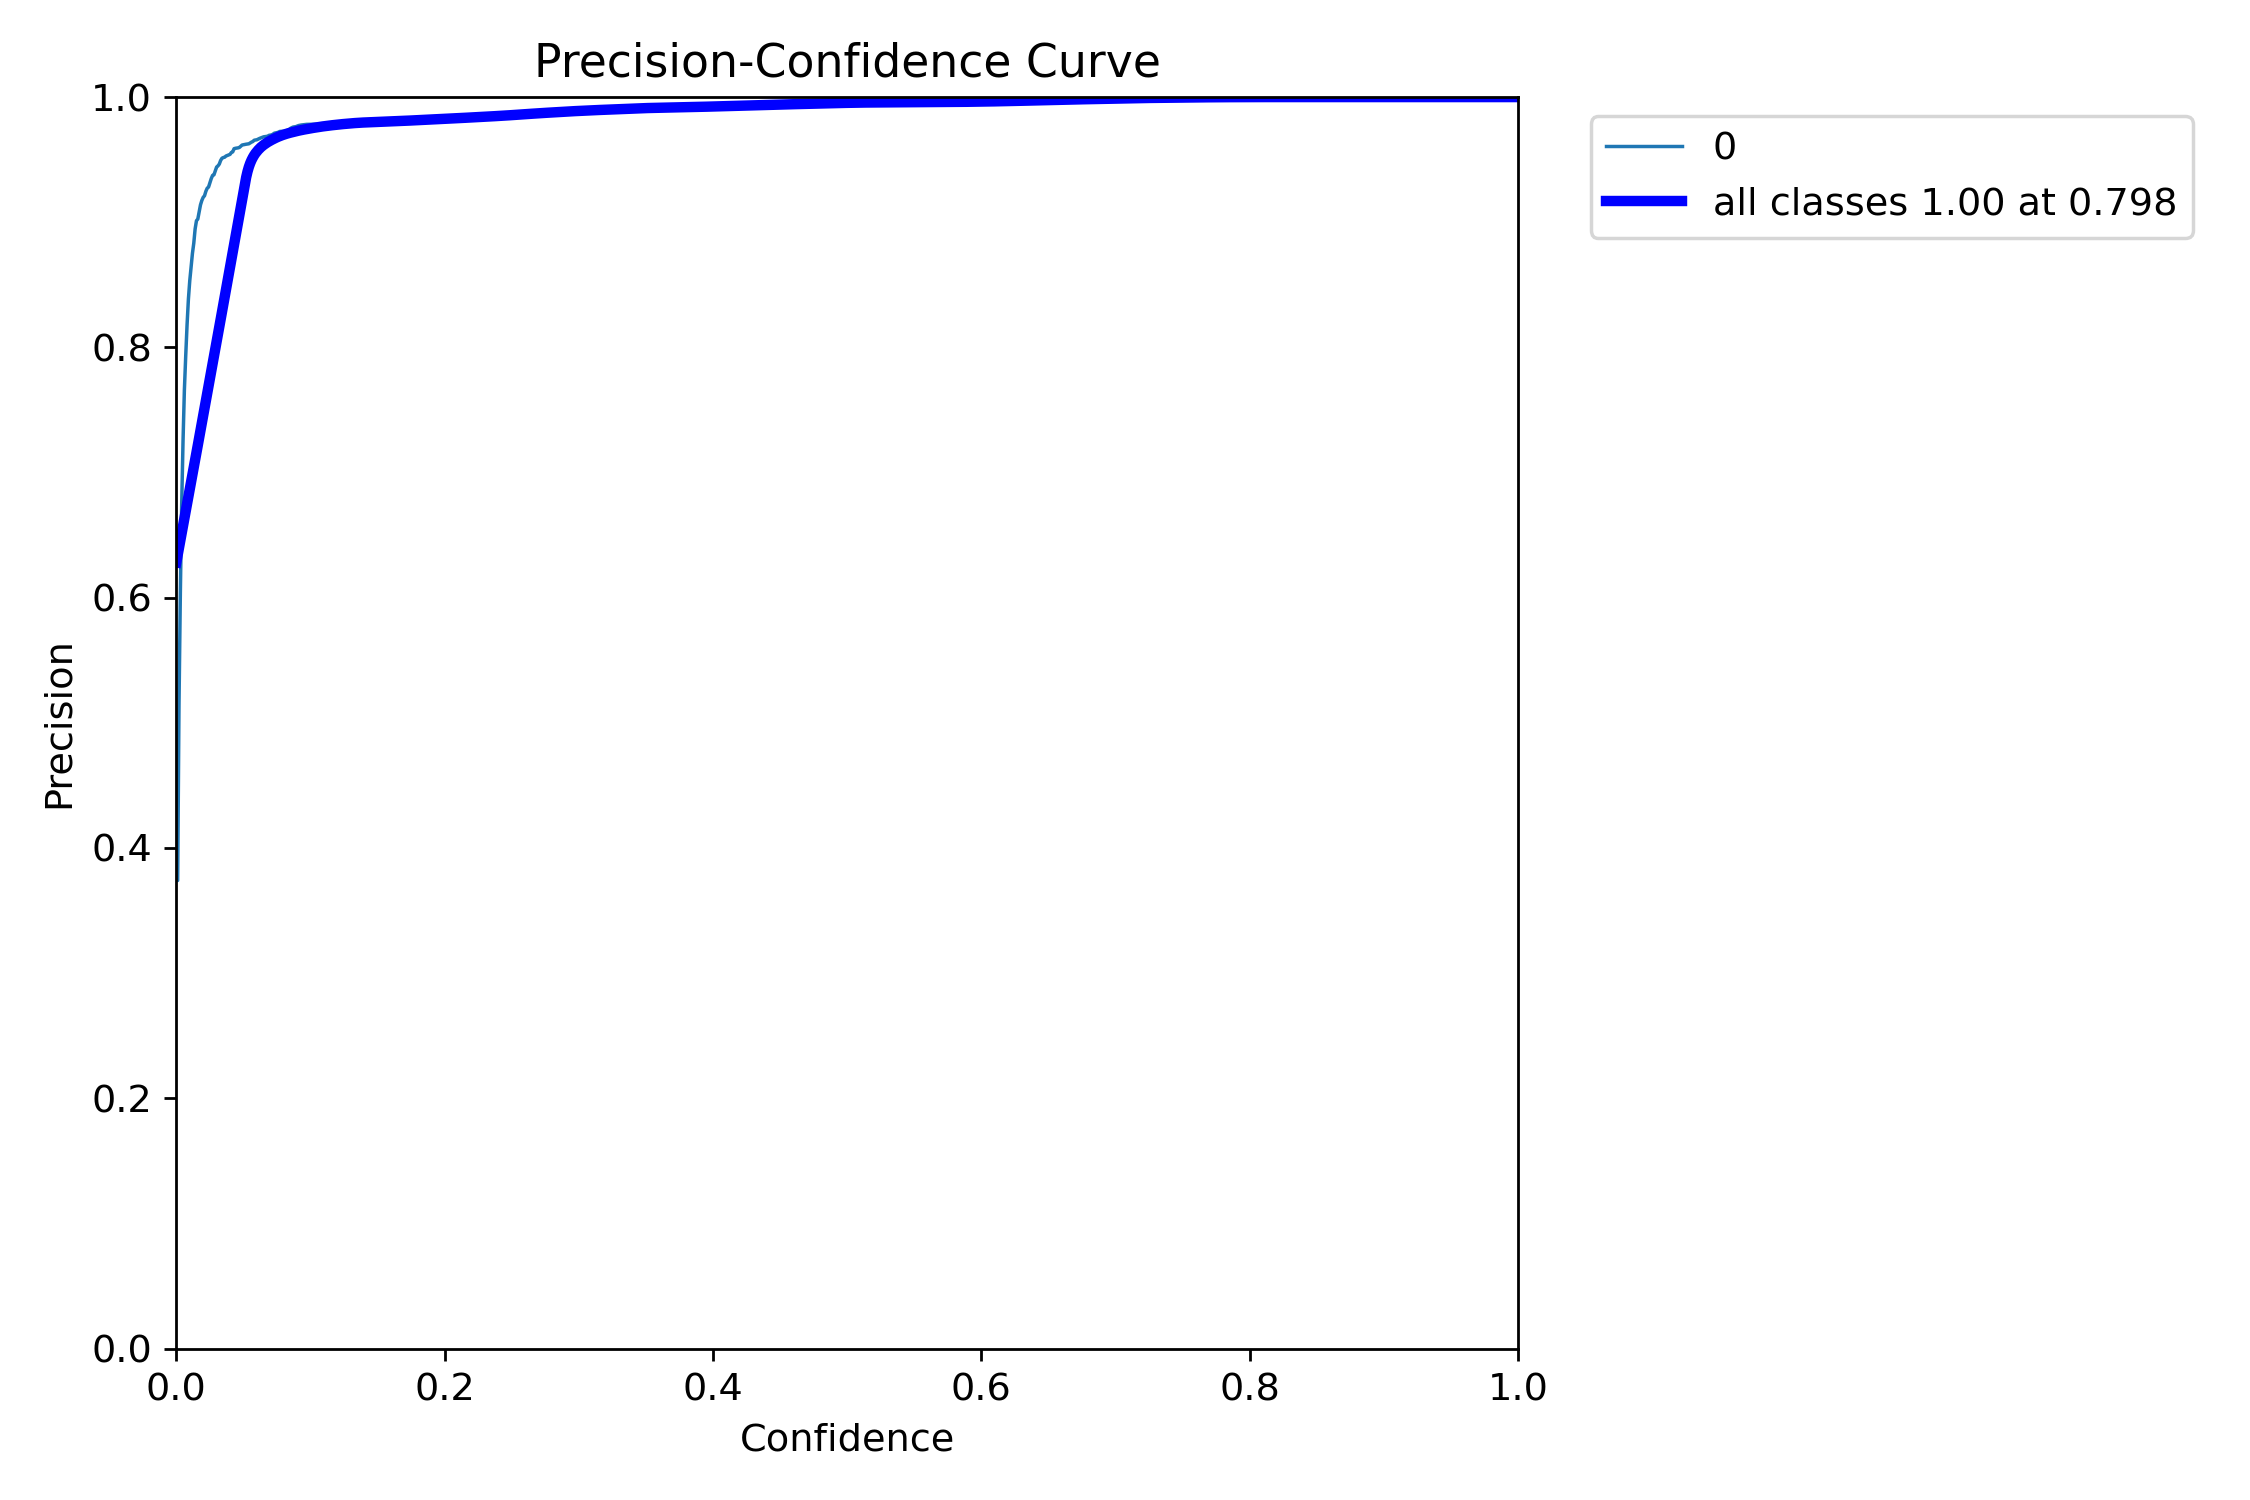
\includegraphics[width=0.85\textwidth]{BoxP_curve.png}
  \caption{Đường cong Box Precision}
\end{subfigure}
\hfill
\begin{subfigure}[b]{0.48\textwidth}
  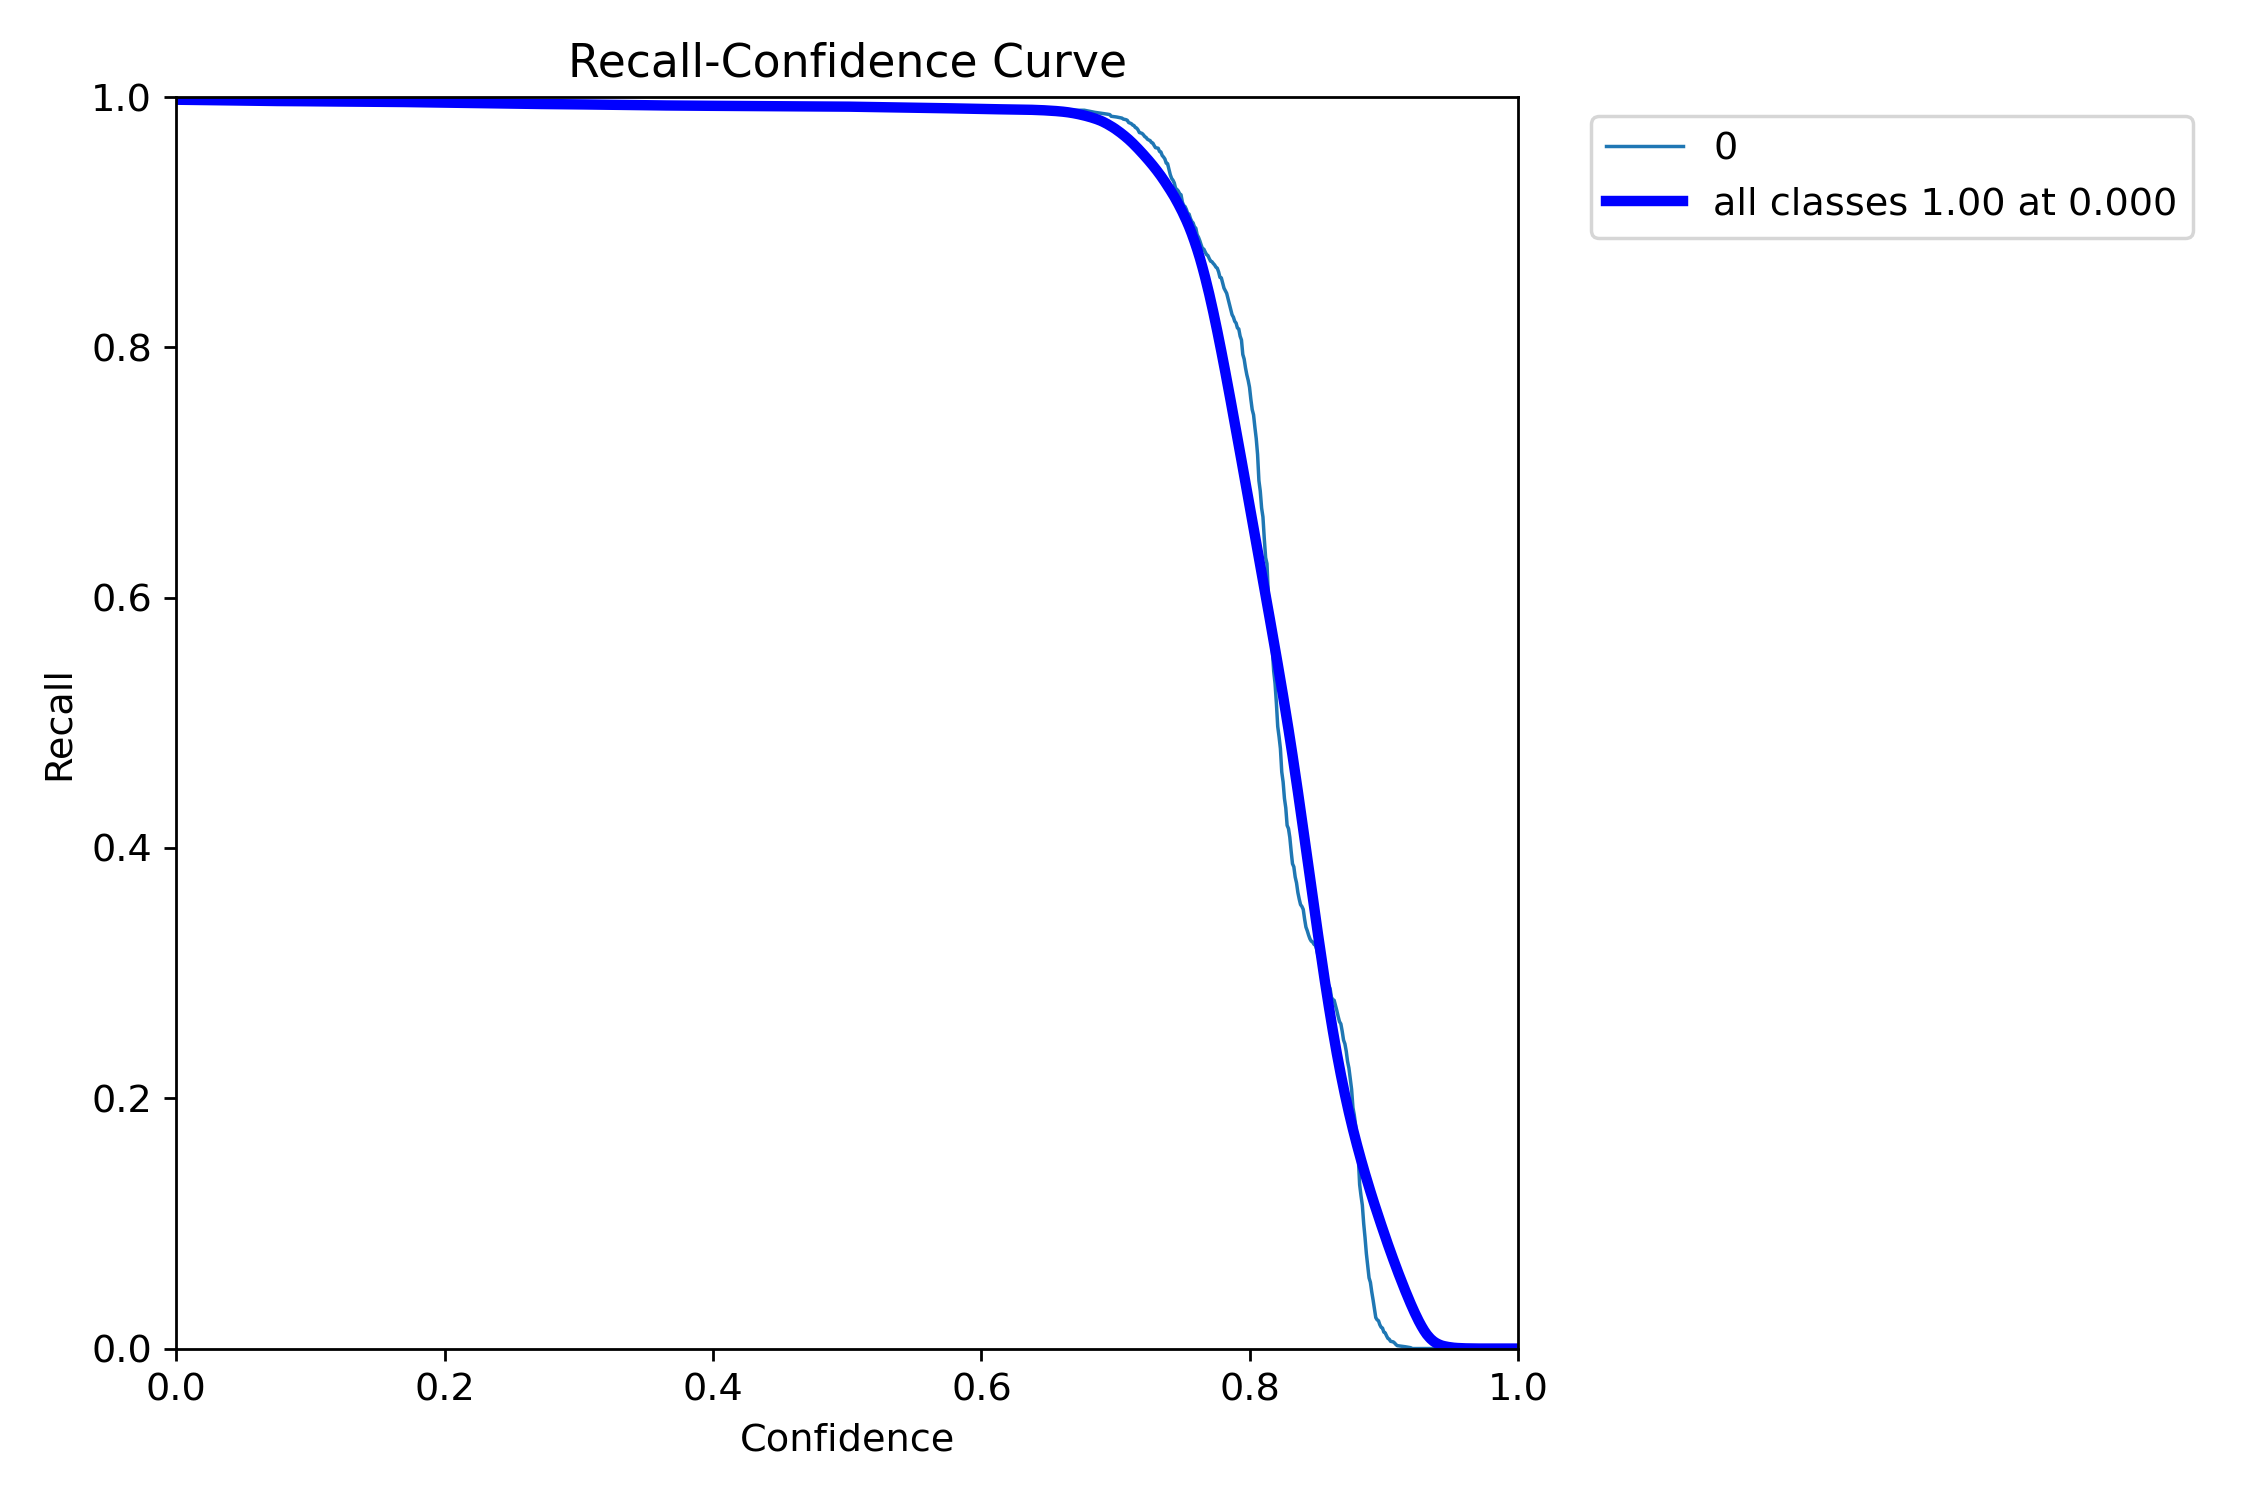
\includegraphics[width=0.85\textwidth]{BoxR_curve.png}
  \caption{Đường cong Box Recall}
\end{subfigure}
\caption{Đường cong Precision và Recall theo epoch}
\label{fig:pr_curves}
\end{figure}

\begin{figure}[H]
\centering
\begin{subfigure}[b]{0.48\textwidth}
  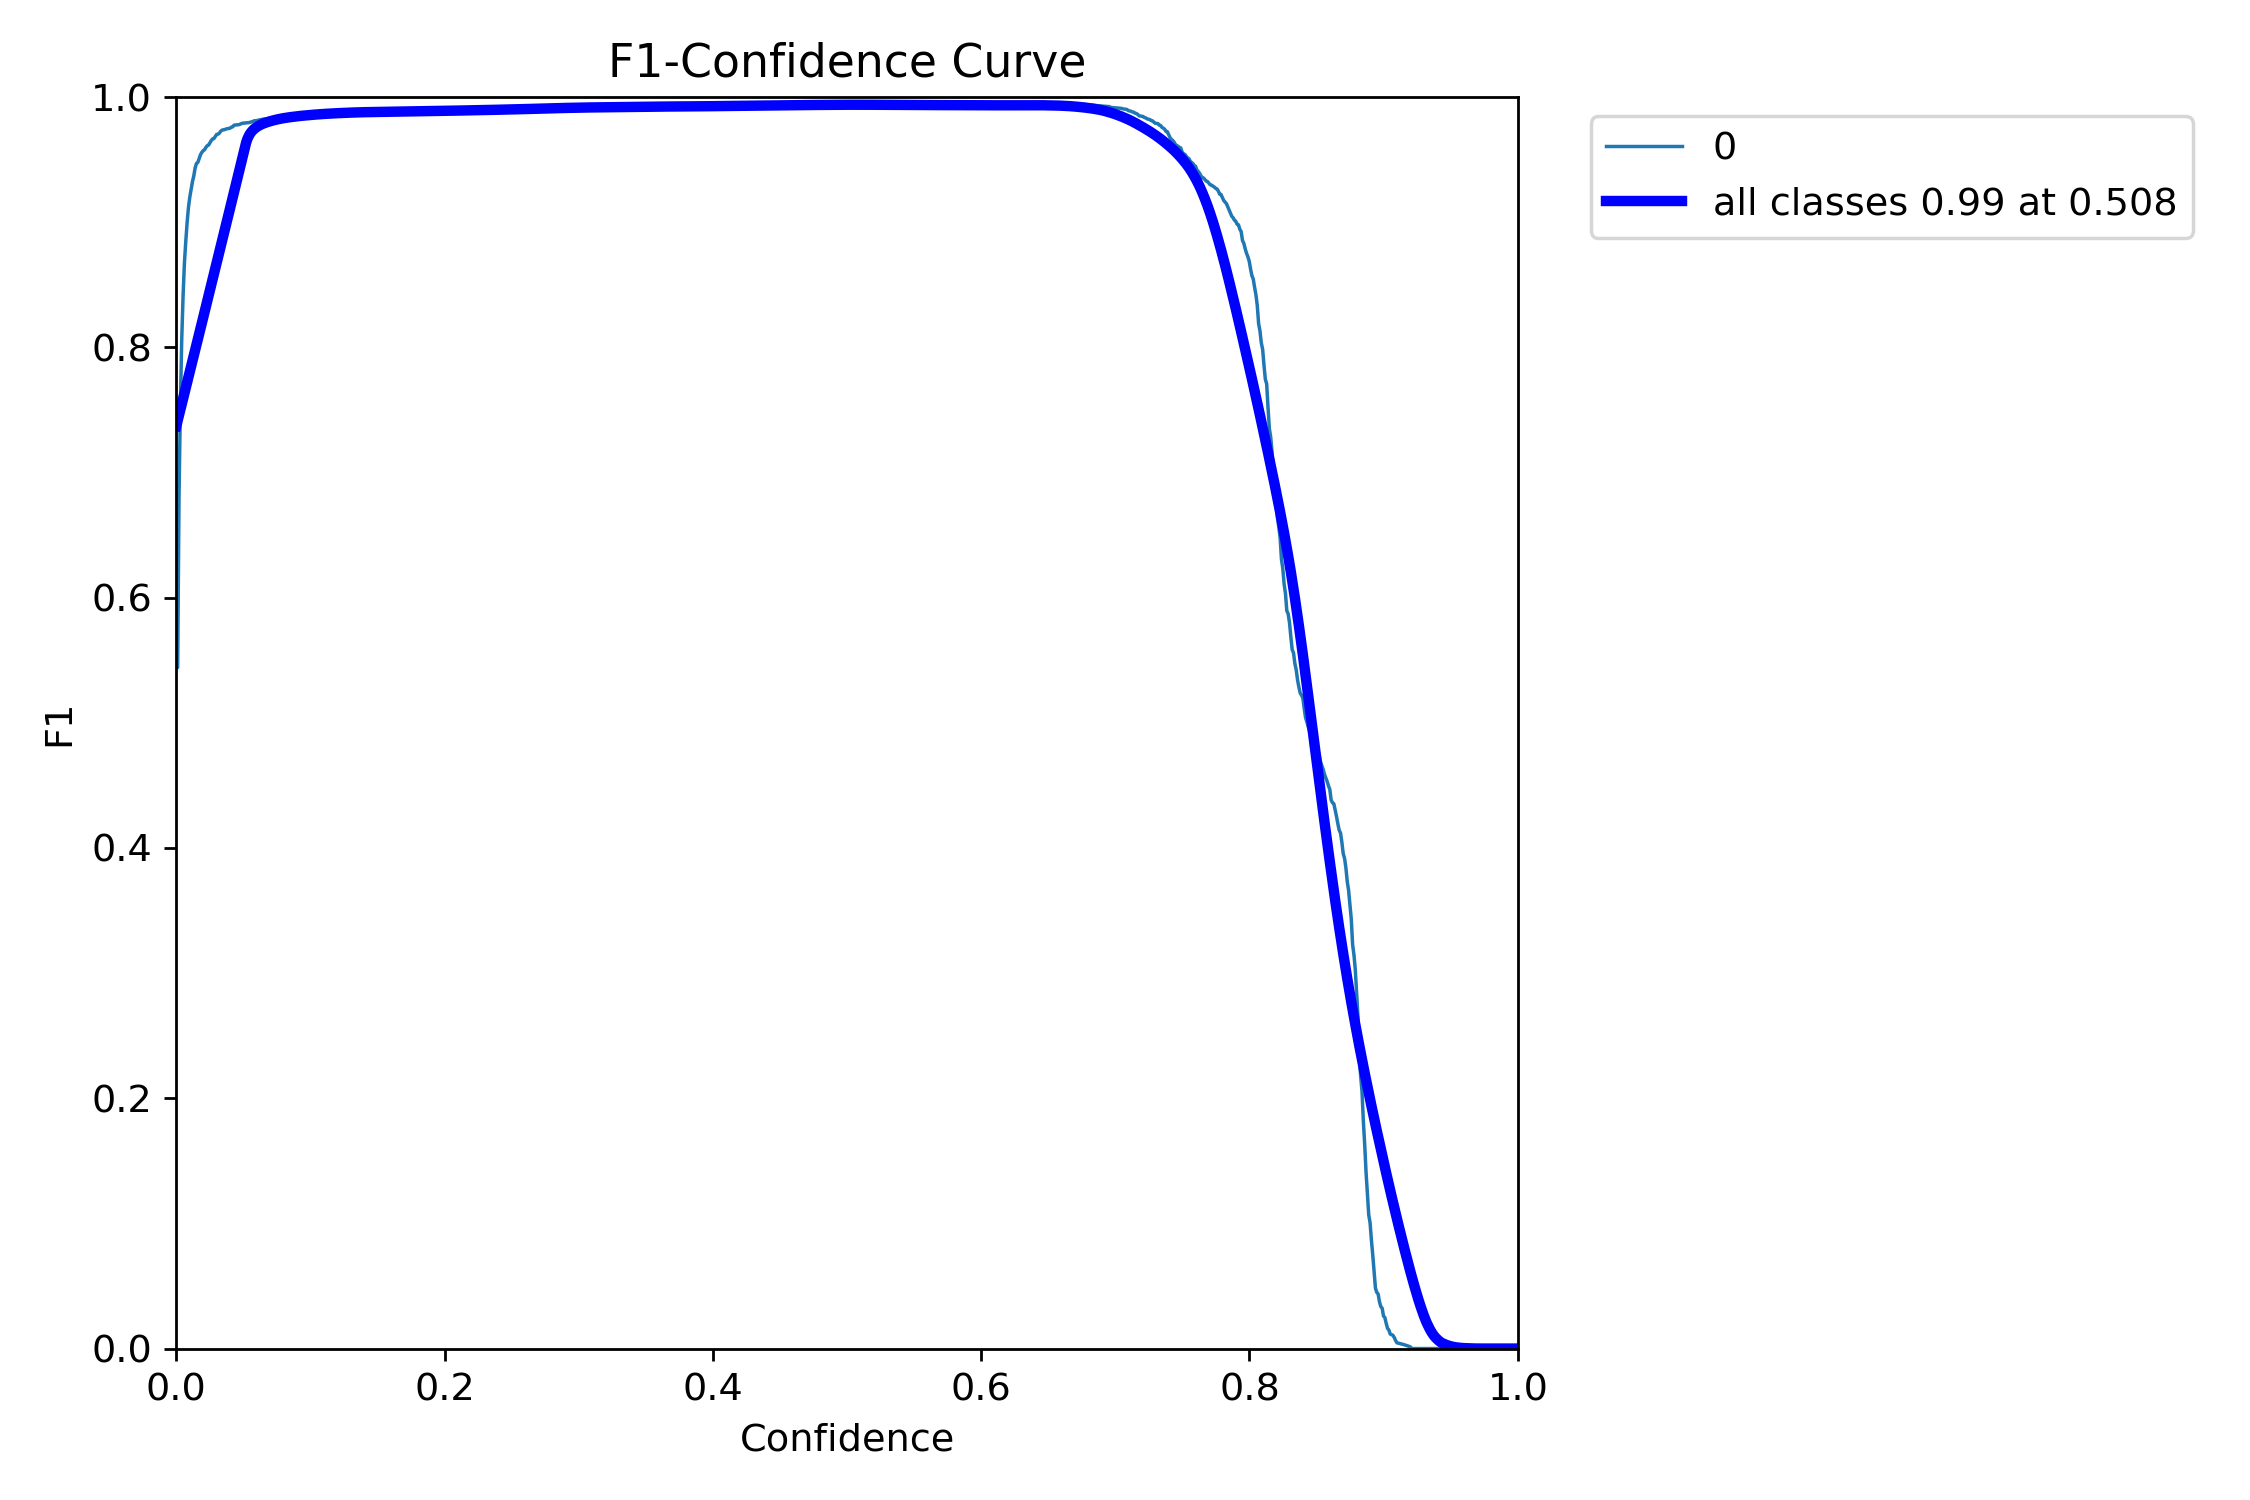
\includegraphics[width=0.85\textwidth]{BoxF1_curve.png}
  \caption{Đường cong F1-Score}
\end{subfigure}
\hfill
\begin{subfigure}[b]{0.48\textwidth}
  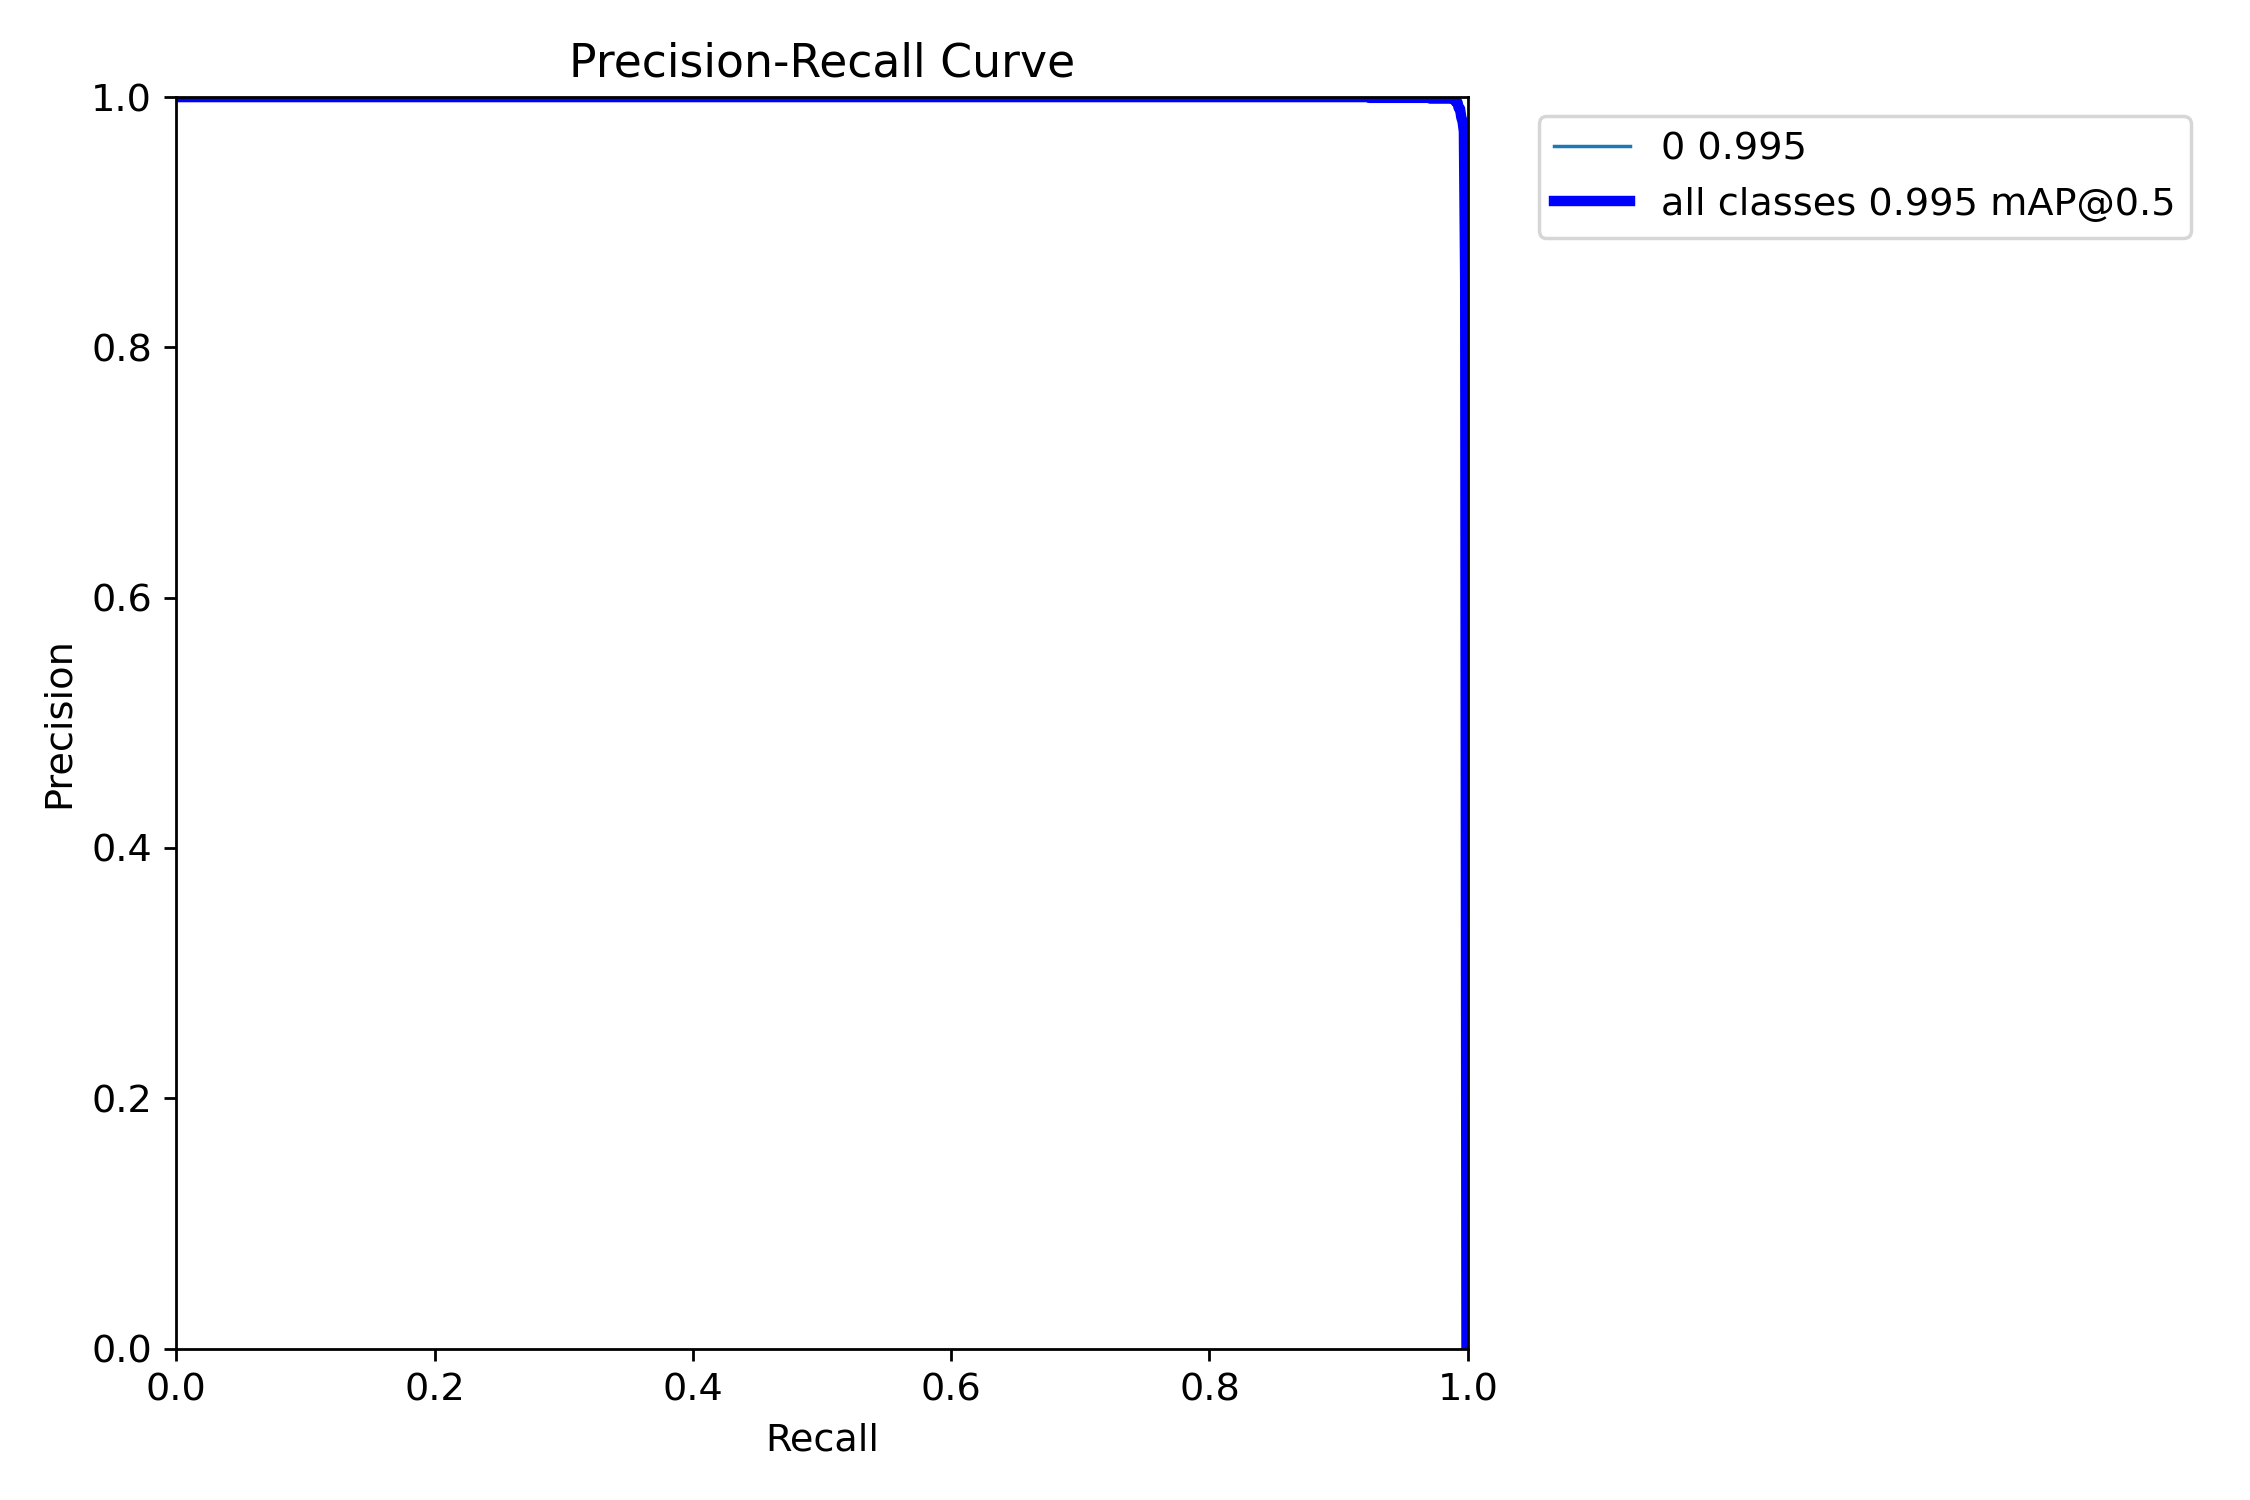
\includegraphics[width=0.85\textwidth]{BoxPR_curve.png}
  \caption{Đường cong Precision-Recall}
\end{subfigure}
\caption{Đường cong F1-Score và PR Curve}
\label{fig:f1_pr}
\end{figure}

F1-Score đạt đỉnh ở ngưỡng confidence phù hợp. Đường PR gần như vuông góc ở góc trên bên phải, xác nhận mAP50 rất cao ($\sim$99.48\%).

\subsection{Ma trận nhầm lẫn YOLOv8}

\begin{figure}[H]
\centering
\begin{subfigure}[b]{0.48\textwidth}
  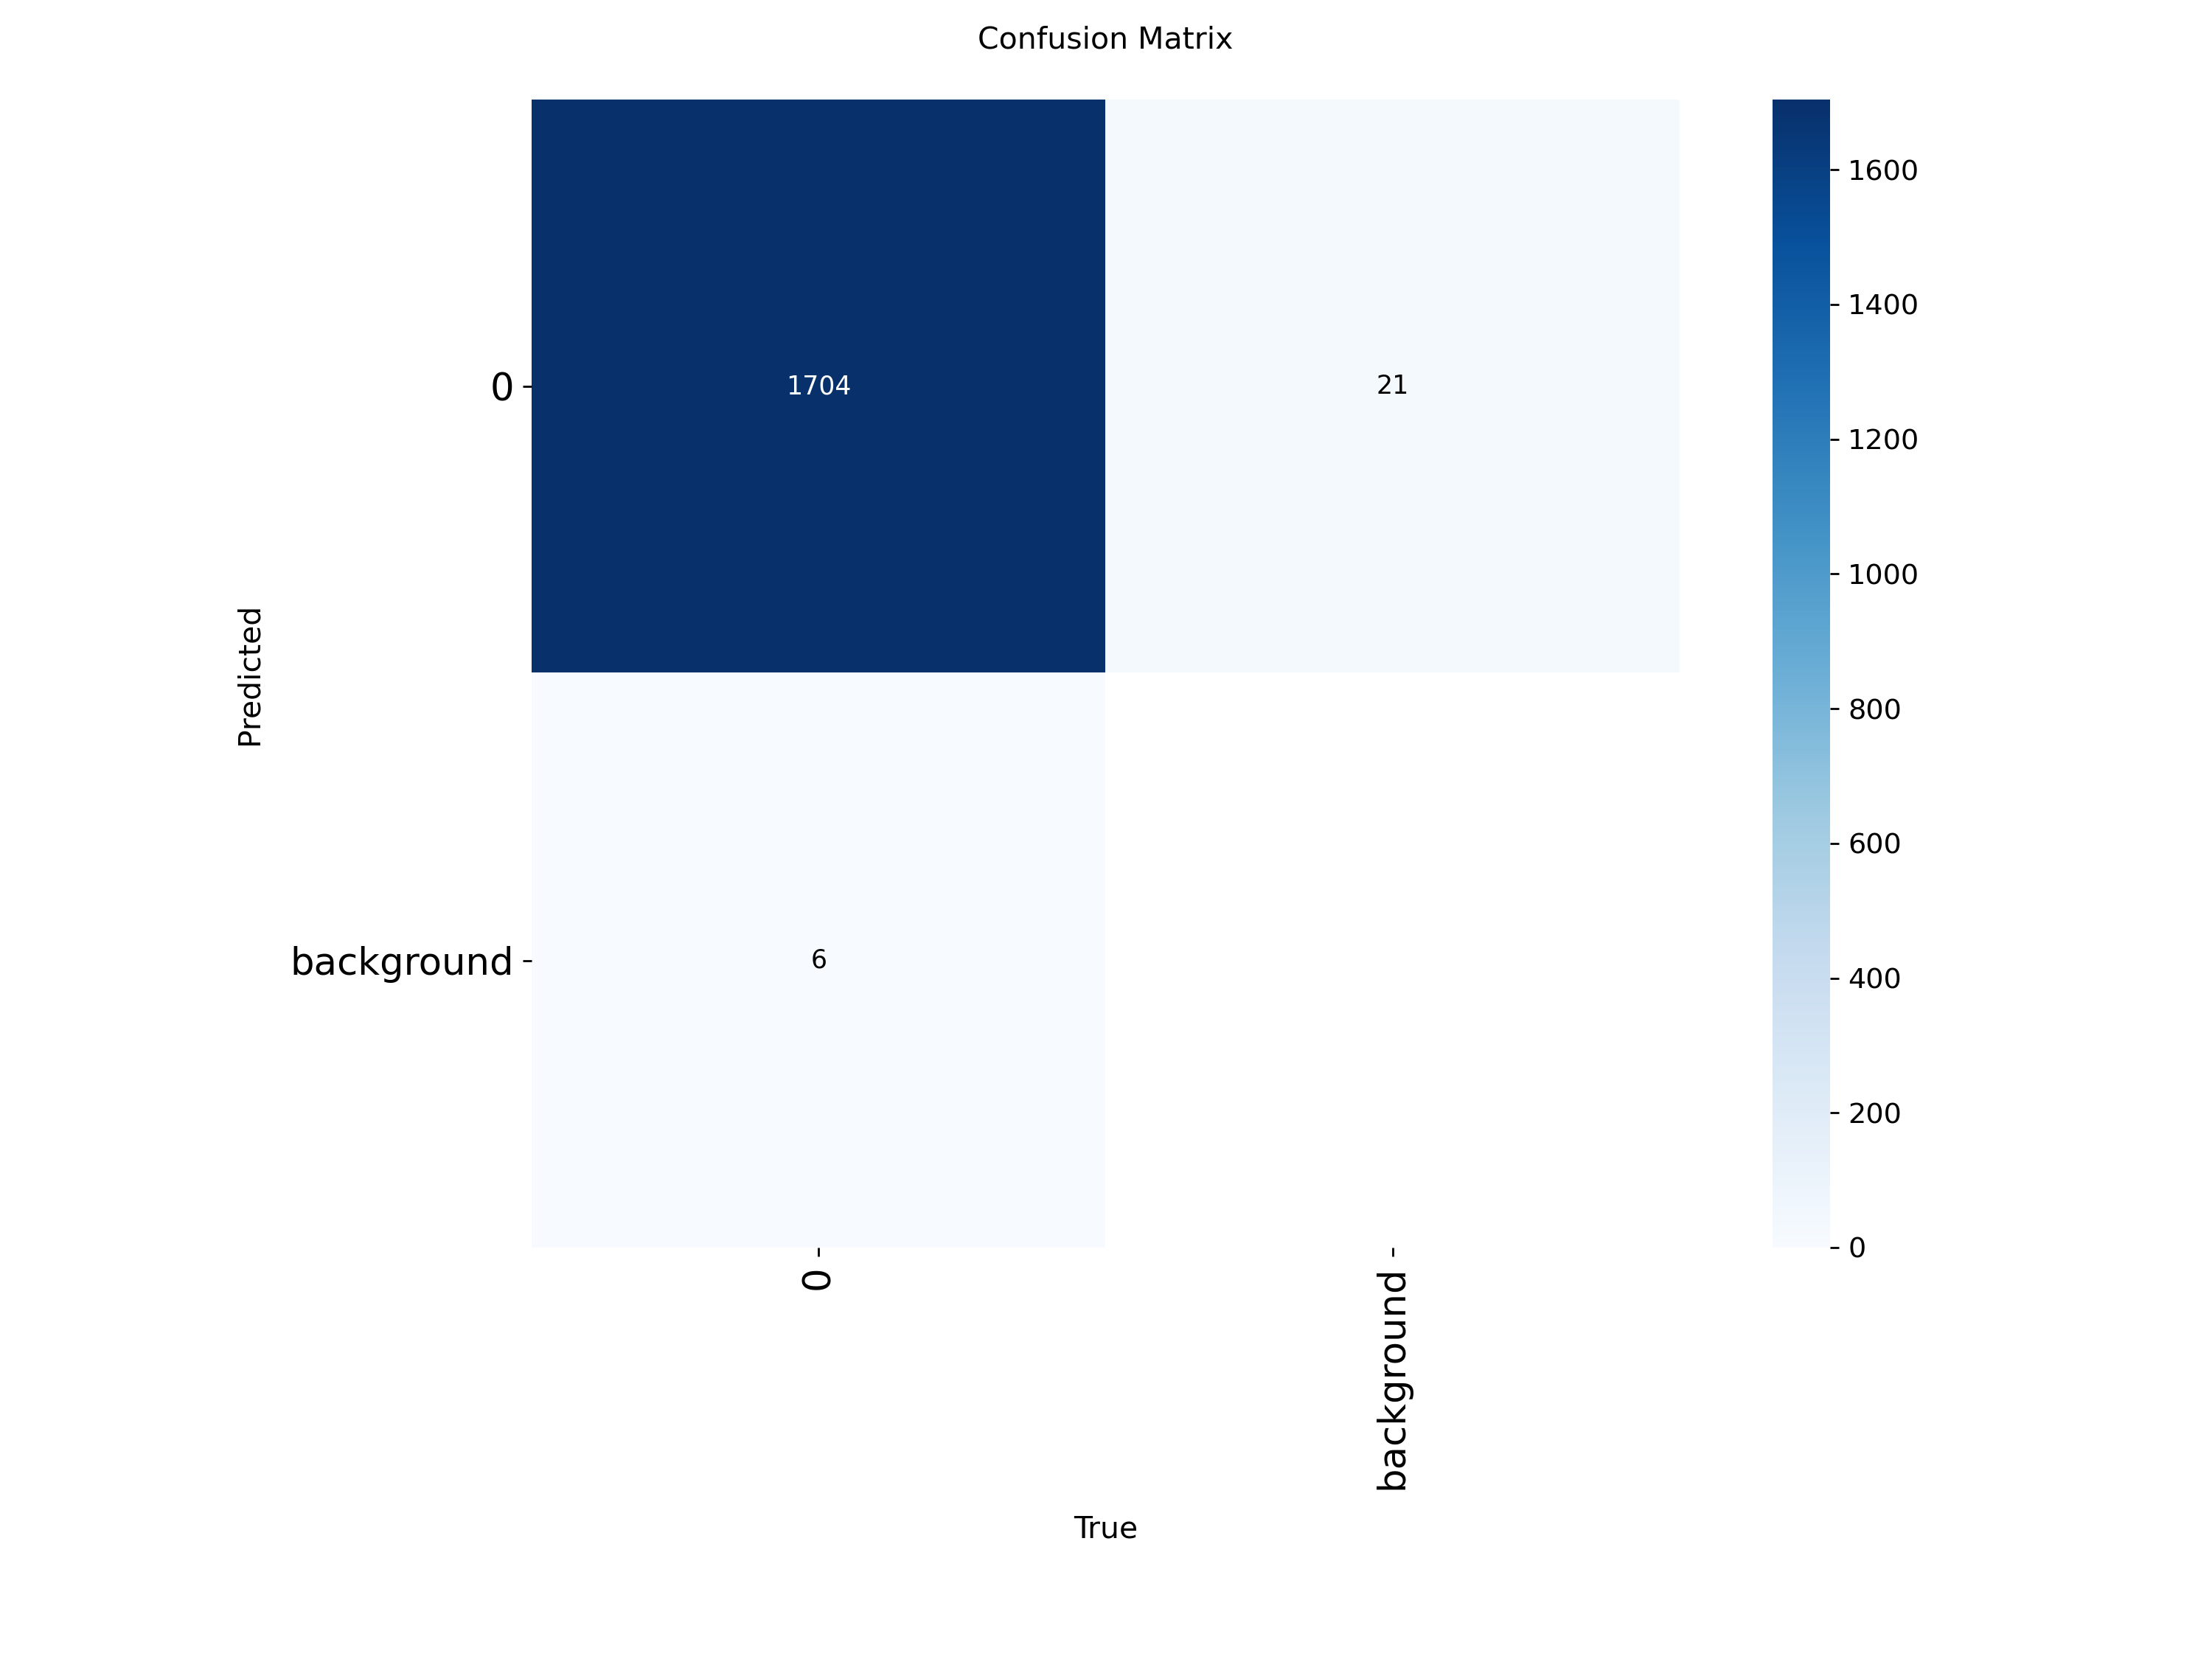
\includegraphics[width=0.85\textwidth]{confusion_matrix.png}
  \caption{Giá trị tuyệt đối}
\end{subfigure}
\hfill
\begin{subfigure}[b]{0.48\textwidth}
  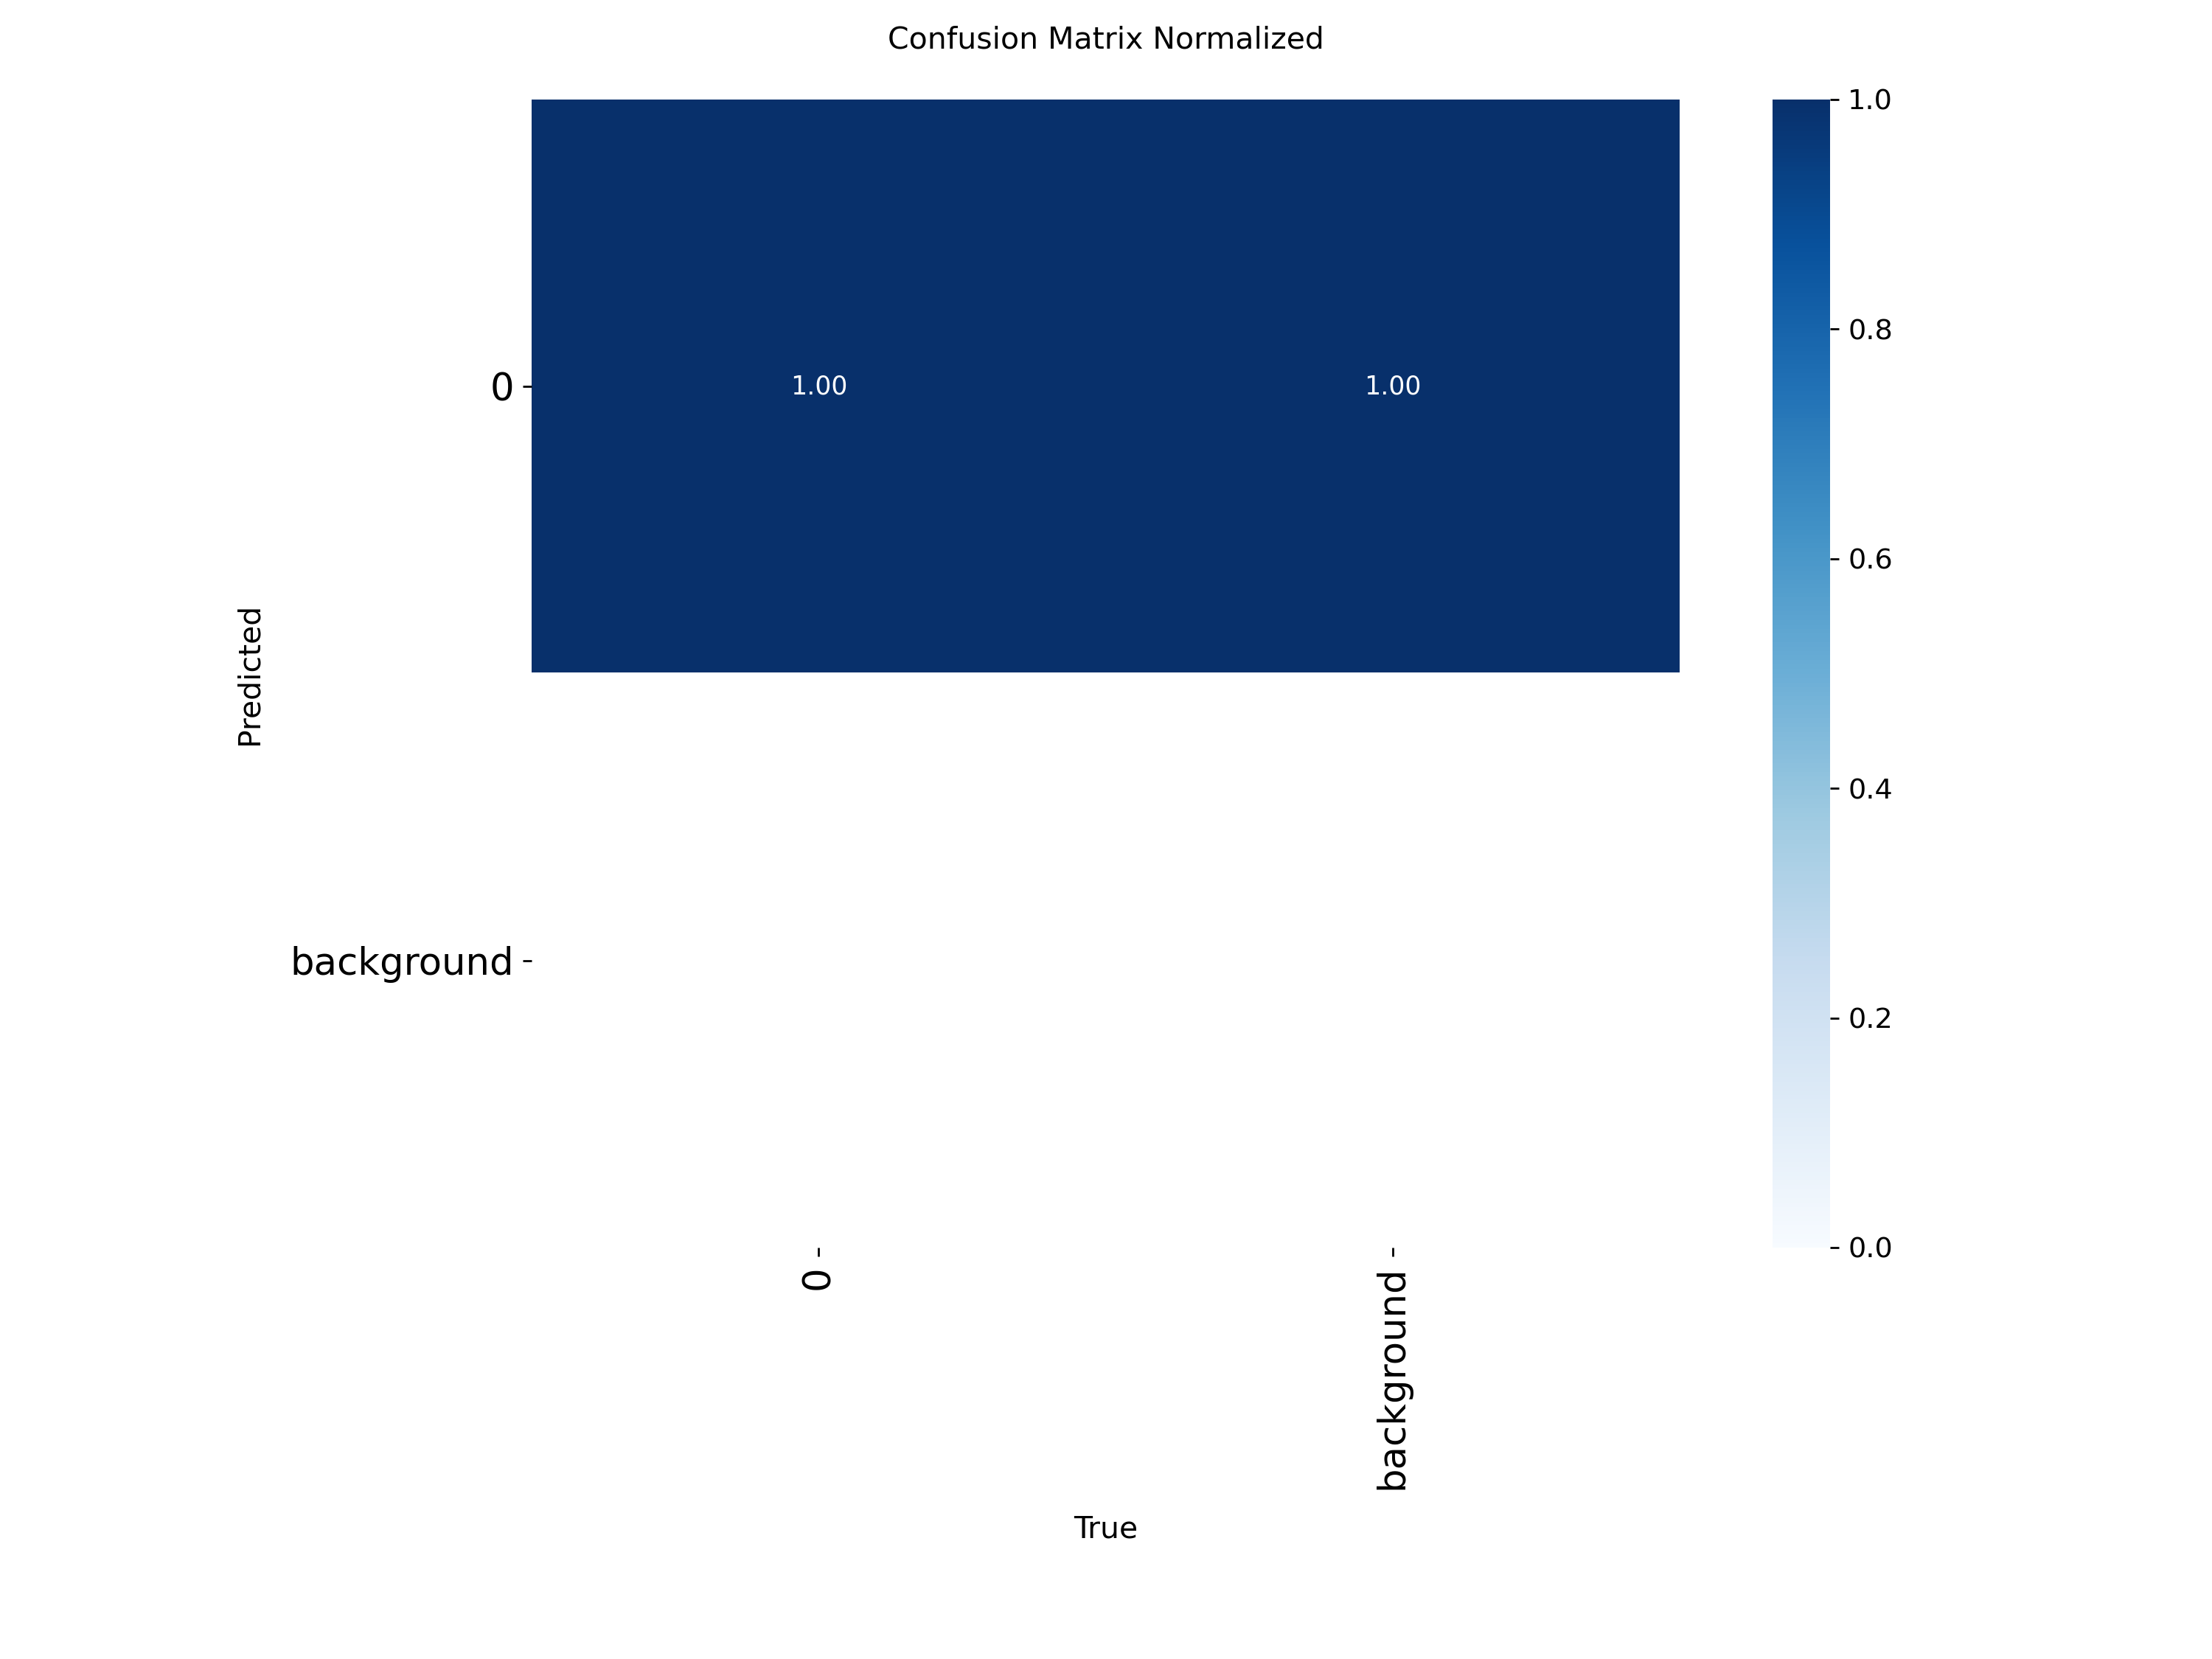
\includegraphics[width=0.85\textwidth]{confusion_matrix_normalized.png}
  \caption{Chuẩn hóa}
\end{subfigure}
\caption{Ma trận nhầm lẫn YOLOv8}
\label{fig:cm_yolo}
\end{figure}

Ma trận nhầm lẫn cho thấy mô hình YOLO hầu như không nhầm lẫn. Tỷ lệ dự đoán đúng lớp \texttt{license\_plate} gần 100\%, với rất ít false negative hoặc false positive.

\subsection{Phân bố nhãn trong dataset}

\begin{figure}[H]
\centering
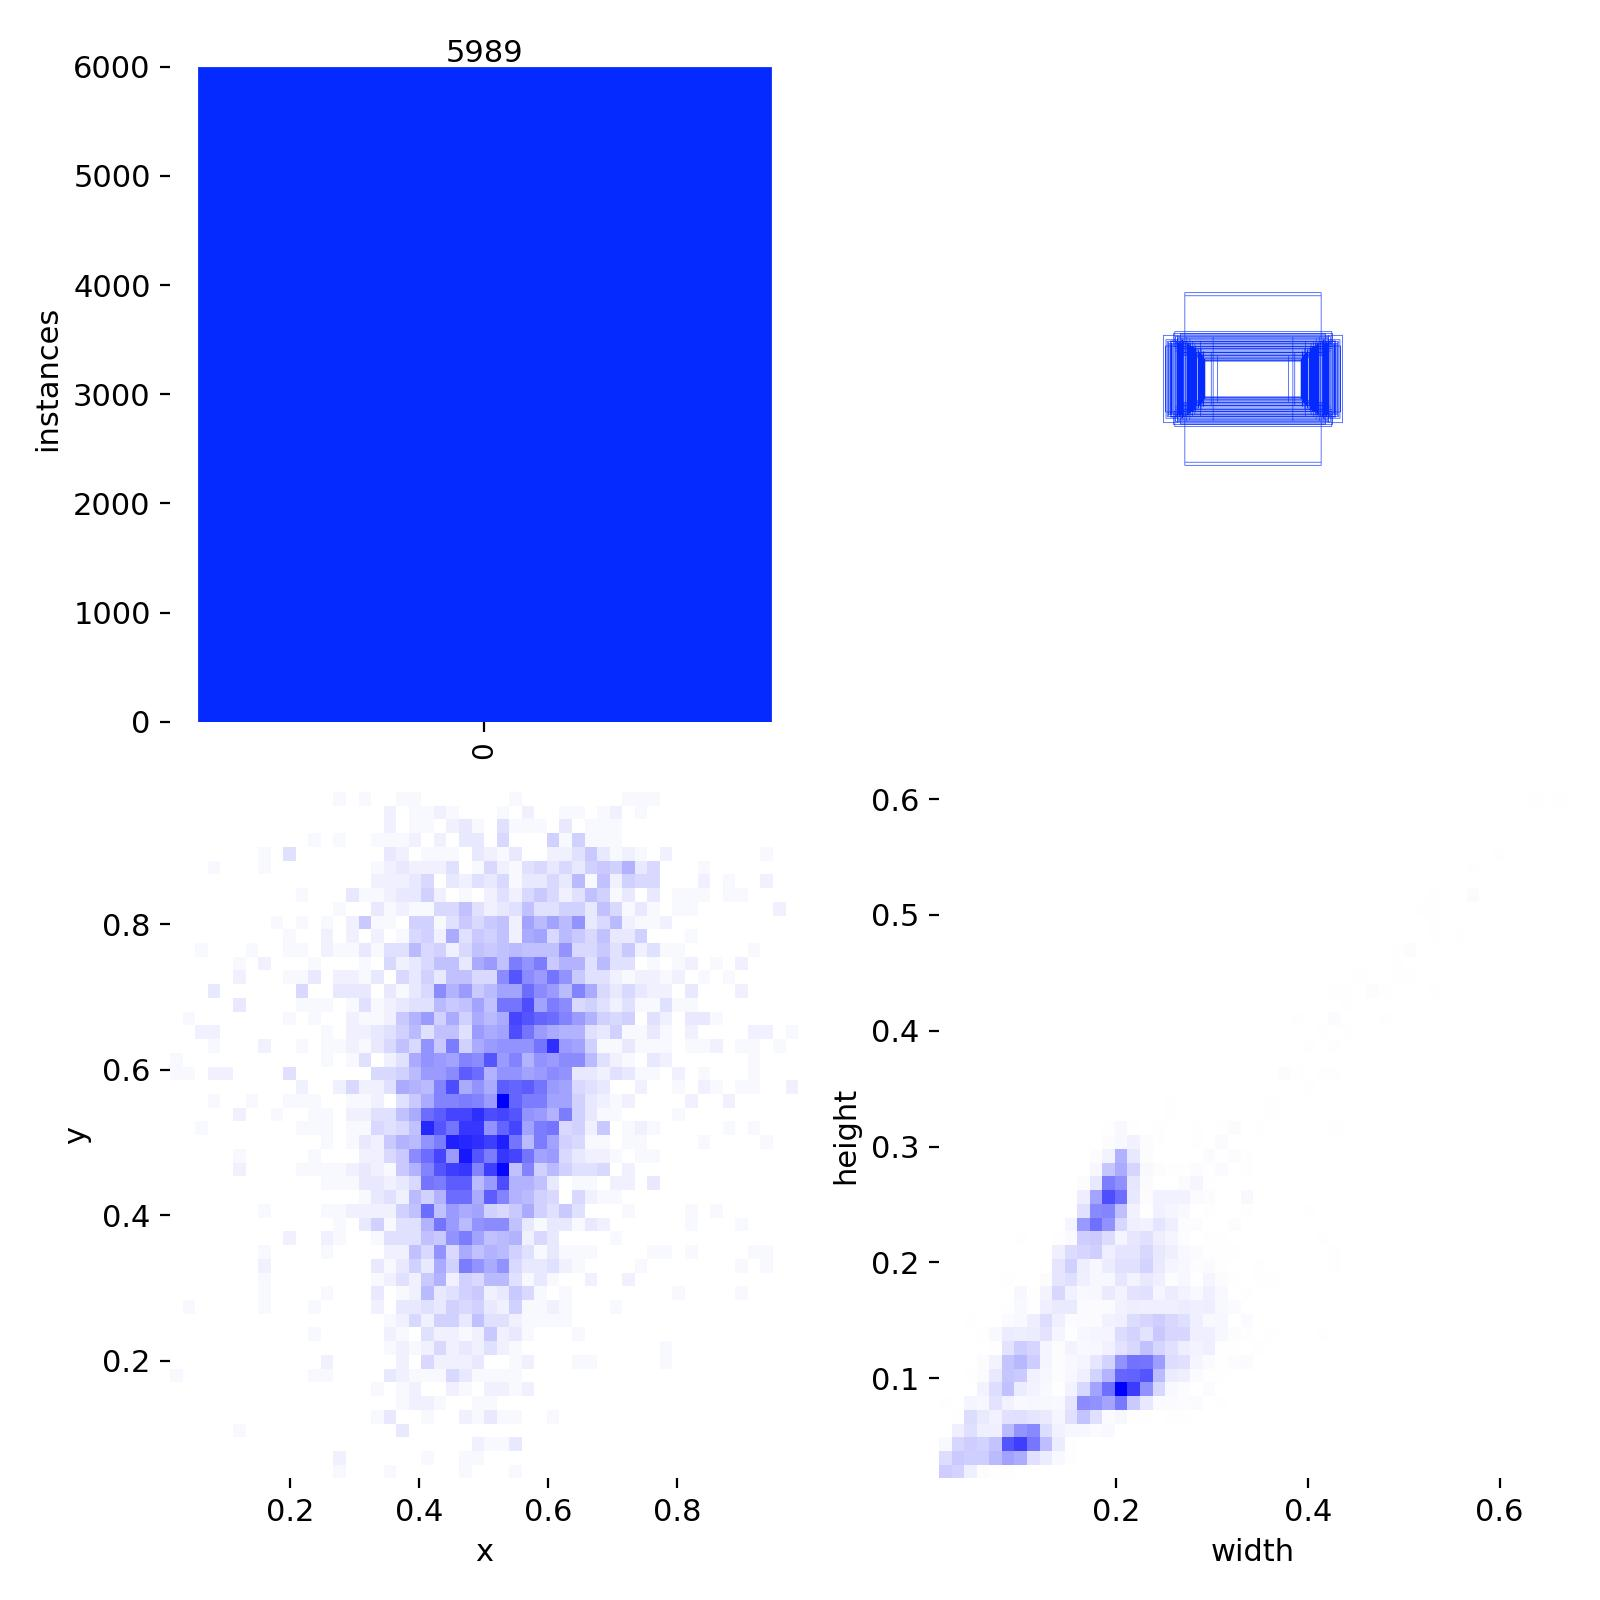
\includegraphics[width=0.85\textwidth]{labels.jpg}
\caption{Phân bố nhãn và kích thước bounding box trong dataset}
\label{fig:labels}
\end{figure}

\subsection{Kết quả validation}

\begin{figure}[H]
\centering
\begin{subfigure}[b]{0.48\textwidth}
  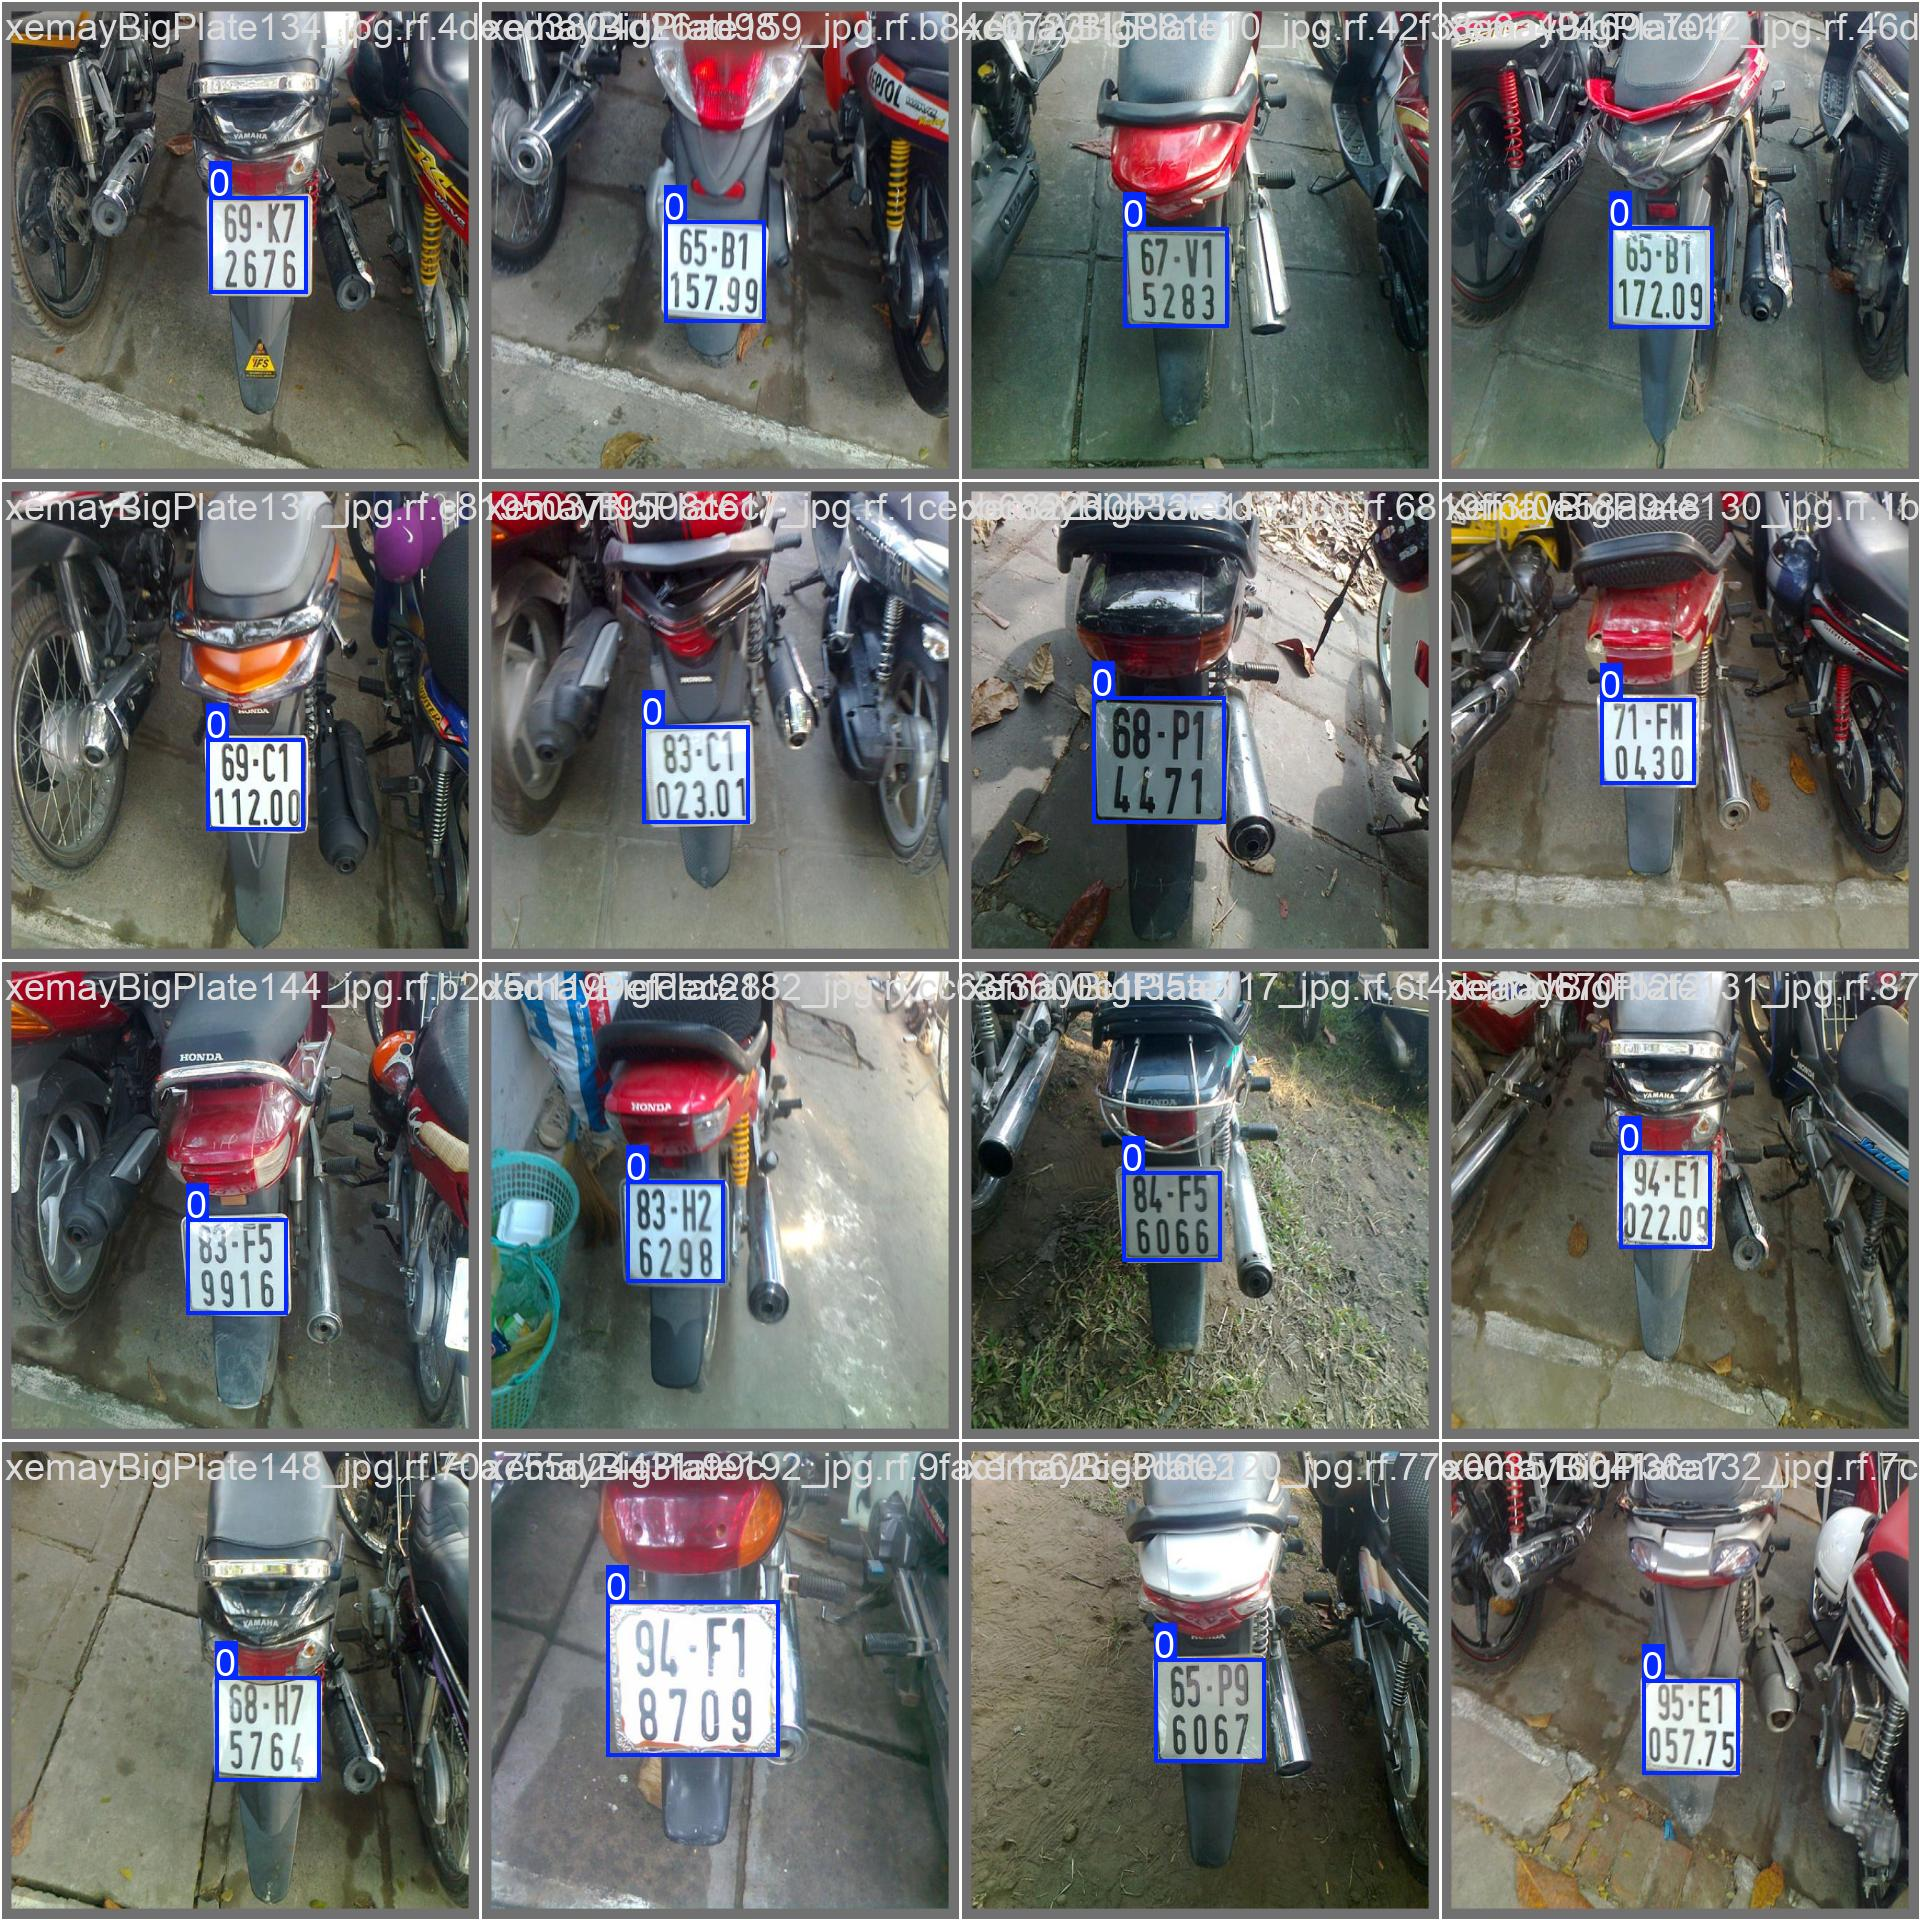
\includegraphics[width=0.85\textwidth]{val_batch0_labels.jpg}
  \caption{Nhãn thực tế (Ground Truth)}
\end{subfigure}
\hfill
\begin{subfigure}[b]{0.48\textwidth}
  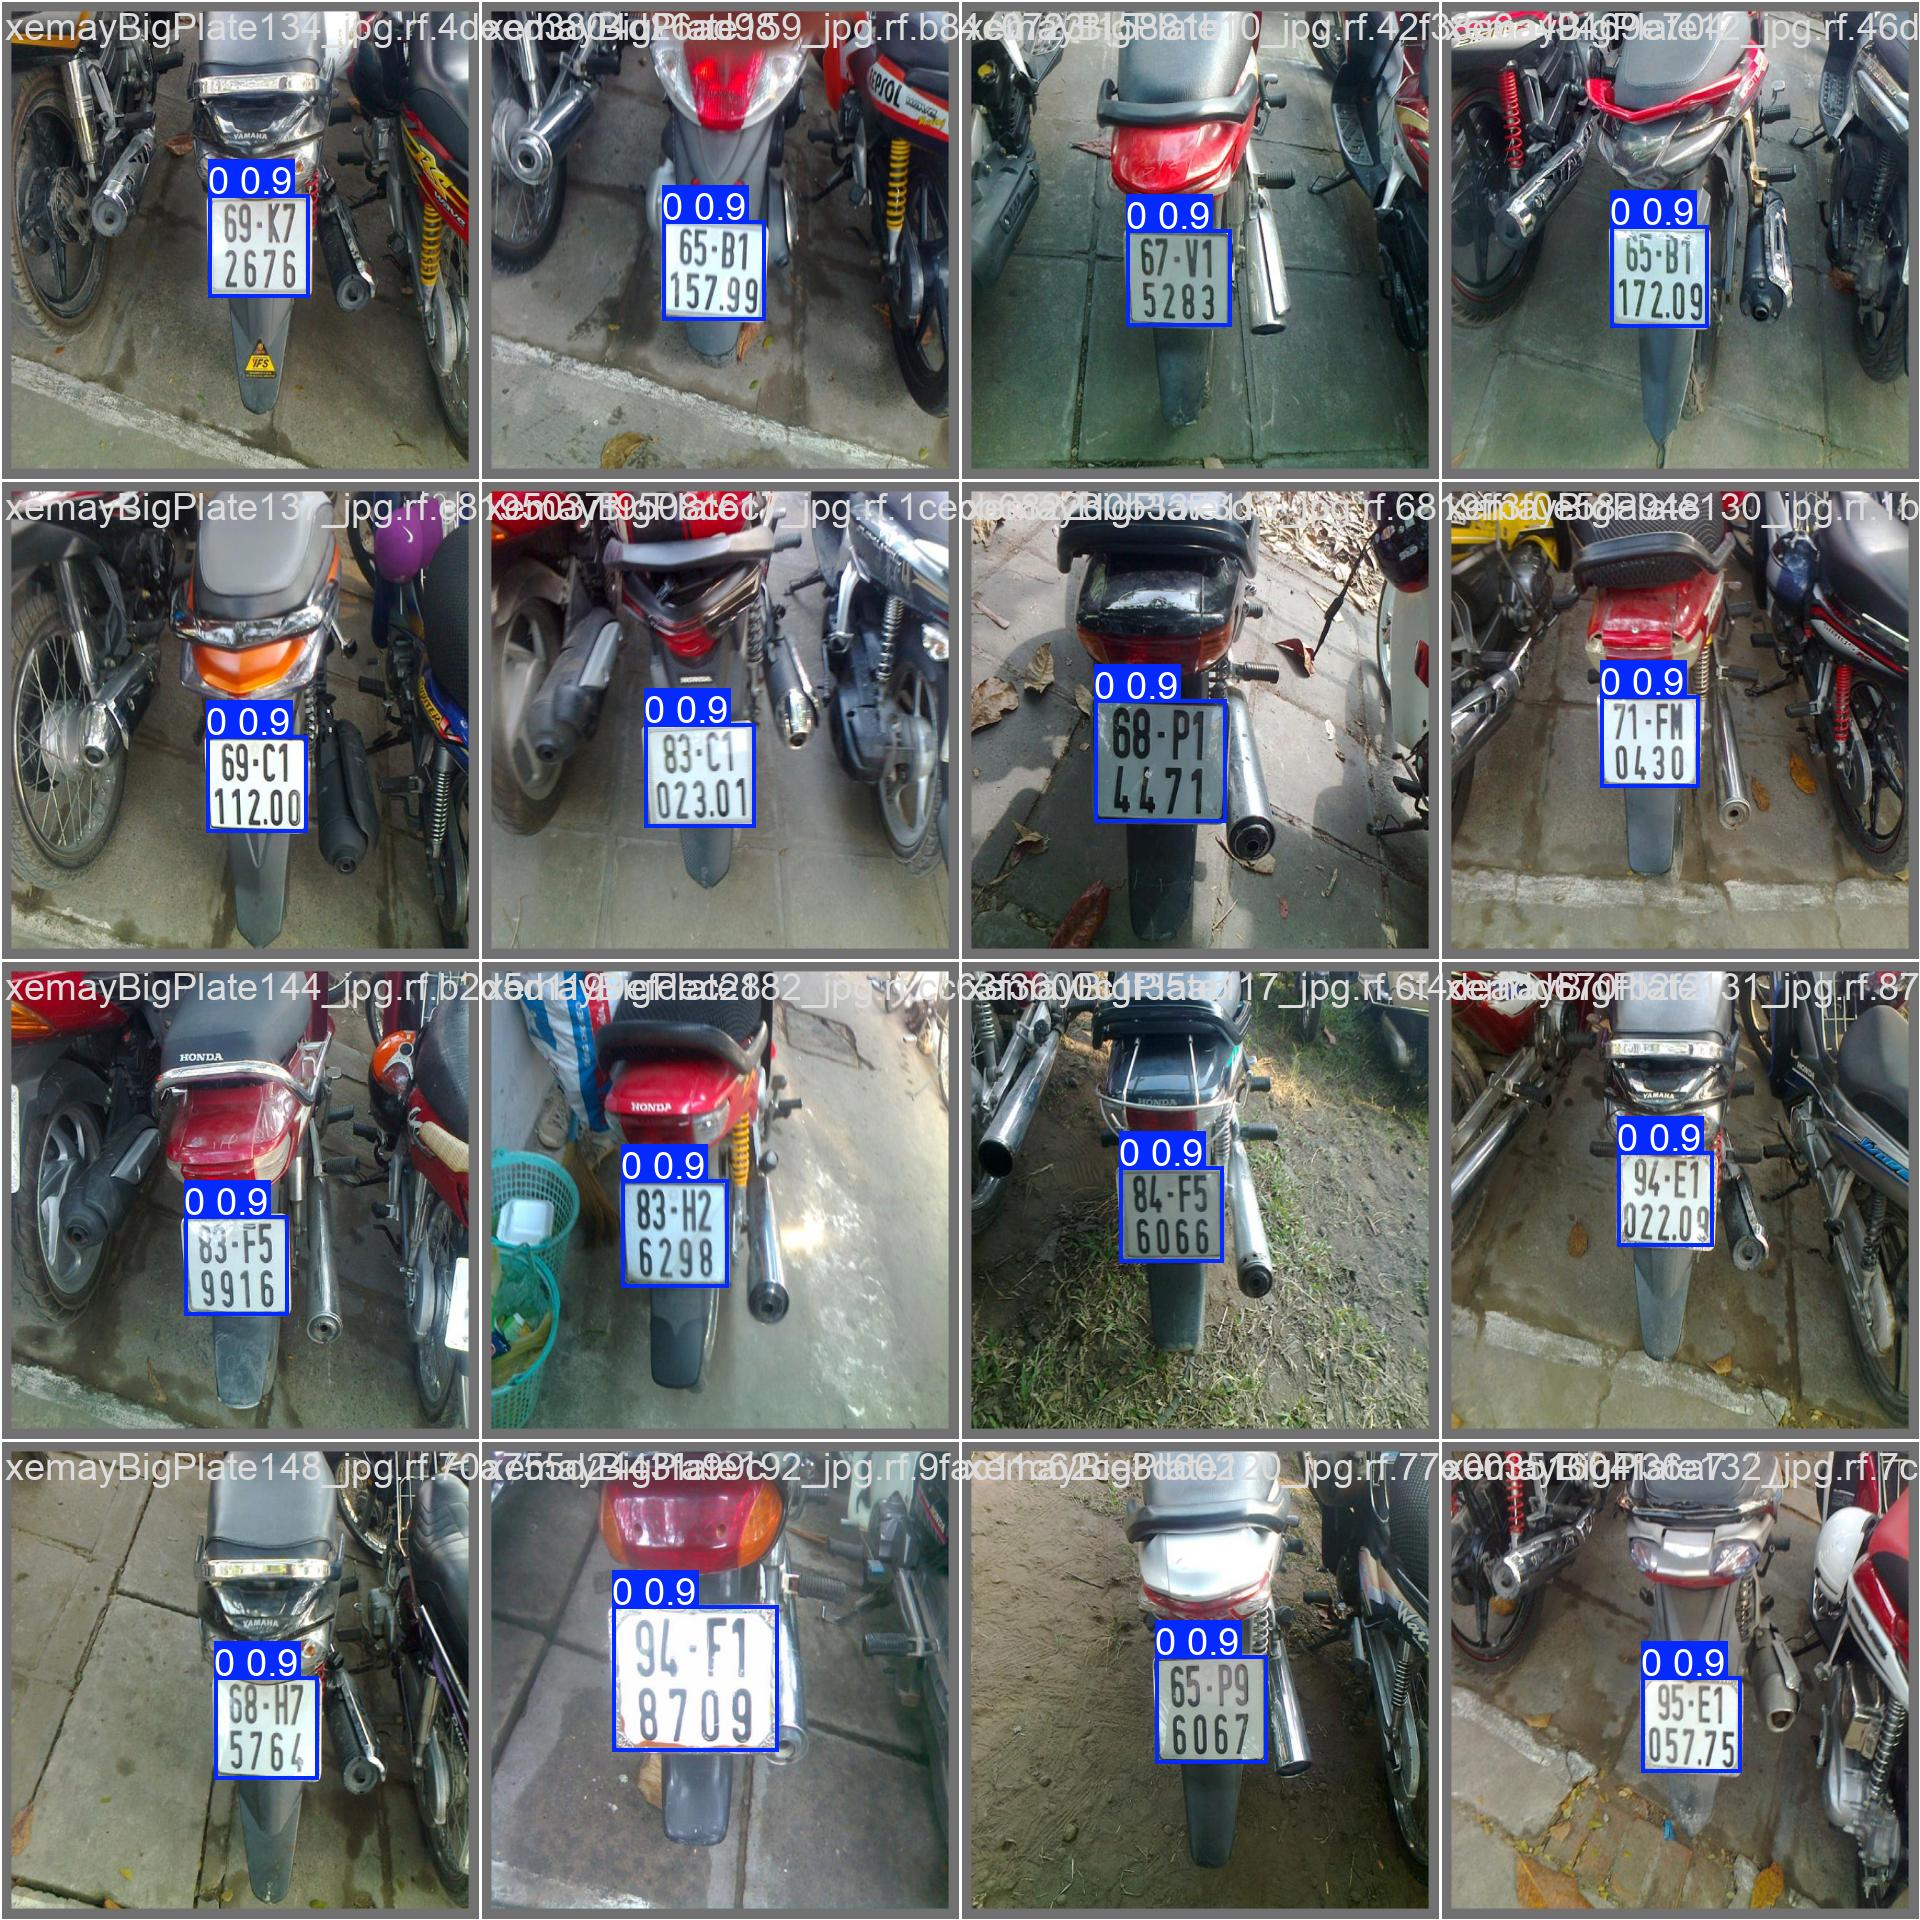
\includegraphics[width=0.85\textwidth]{val_batch0_pred.jpg}
  \caption{Kết quả dự đoán}
\end{subfigure}
\caption{So sánh Ground Truth và Prediction trên tập validation}
\label{fig:val}
\end{figure}

\section{Kết quả nhận diện ký tự (PaddleOCR)}

\subsection{So sánh phương pháp tiền xử lý ảnh}

\begin{table}[H]
\centering
\caption{So sánh phương pháp tiền xử lý ảnh}
\label{tab:tien_xu_ly}
\begin{tabular}{lrr}
\toprule
\textbf{Phương pháp} & \textbf{Accuracy ký tự} & \textbf{Accuracy biển số} \\
\midrule
Ảnh gốc & 99.62\% & 97.00\% \\
CLAHE & 98.56\% & 96.00\% \\
Otsu & 99.19\% & 93.50\% \\
\textbf{Kết hợp chọn tốt nhất} & \textbf{99.69\%} & \textbf{97.50\%} \\
\bottomrule
\end{tabular}
\end{table}

\begin{figure}[H]
\centering
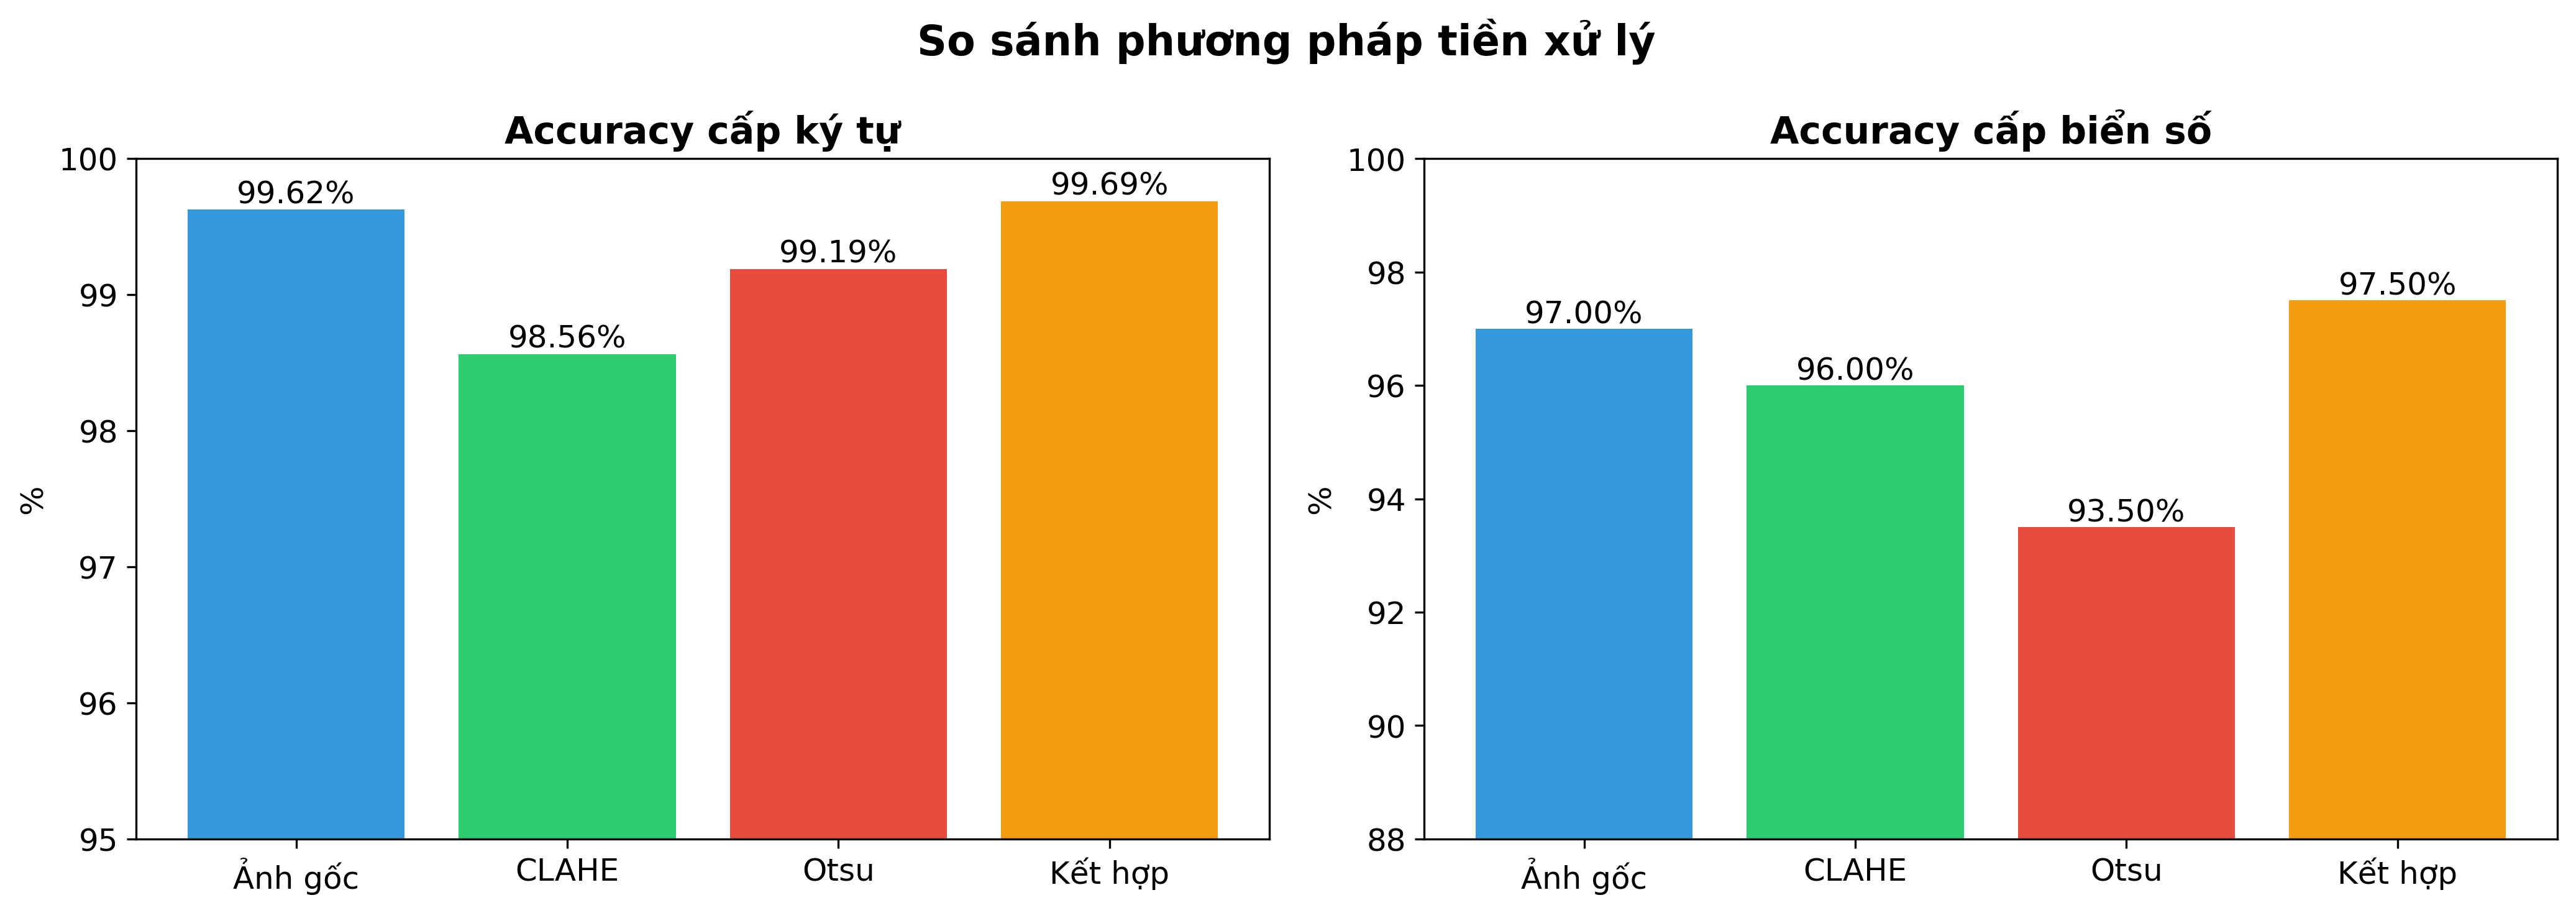
\includegraphics[width=0.85\textwidth]{so_sanh_tien_xu_ly.png}
\caption{Biểu đồ so sánh các phương pháp tiền xử lý ảnh}
\label{fig:ss_tien_xu_ly}
\end{figure}

\subsection{Kết quả hậu xử lý}

Hậu xử lý theo định dạng biển số Việt Nam giúp sửa một số lỗi nhận dạng ký tự và chọn kết quả hợp lý hơn. Kết quả so sánh trước và sau hậu xử lý được trình bày trong Bảng 4.3.

\textbf{Bảng 4.3. So sánh trước và sau hậu xử lý}

Sau hậu xử lý, độ chính xác cấp biển số tăng từ 95.00% lên 97.50%. Điều này cho thấy việc áp dụng quy tắc định dạng biển số Việt Nam có tác dụng tích cực, đặc biệt trong các trường hợp OCR (nhận dạng ký tự quang học) đọc nhầm các ký tự có hình dạng gần giống nhau.


\textbf{Hình 4.2} cho thấy hậu xử lý theo quy tắc biển số Việt Nam giúp tăng độ chính xác, đặc biệt ở cấp biển số hoàn chỉnh. Điều này chứng minh rằng việc kết hợp OCR (nhận dạng ký tự quang học) với luật định dạng thực tế là cần thiết.

\begin{table}[H]
\centering
\caption{So sánh trước và sau hậu xử lý}
\label{tab:hau_xu_ly}
\begin{tabular}{lrrr}
\toprule
\textbf{Chỉ số} & \textbf{Trước} & \textbf{Sau} & \textbf{Cải thiện} \\
\midrule
Accuracy cấp ký tự & 99.44\% & 99.69\% & +0.25\% \\
Accuracy cấp biển số & 95.00\% & 97.50\% & \textbf{+2.50\%} \\
\bottomrule
\end{tabular}
\end{table}

\begin{figure}[H]
\centering
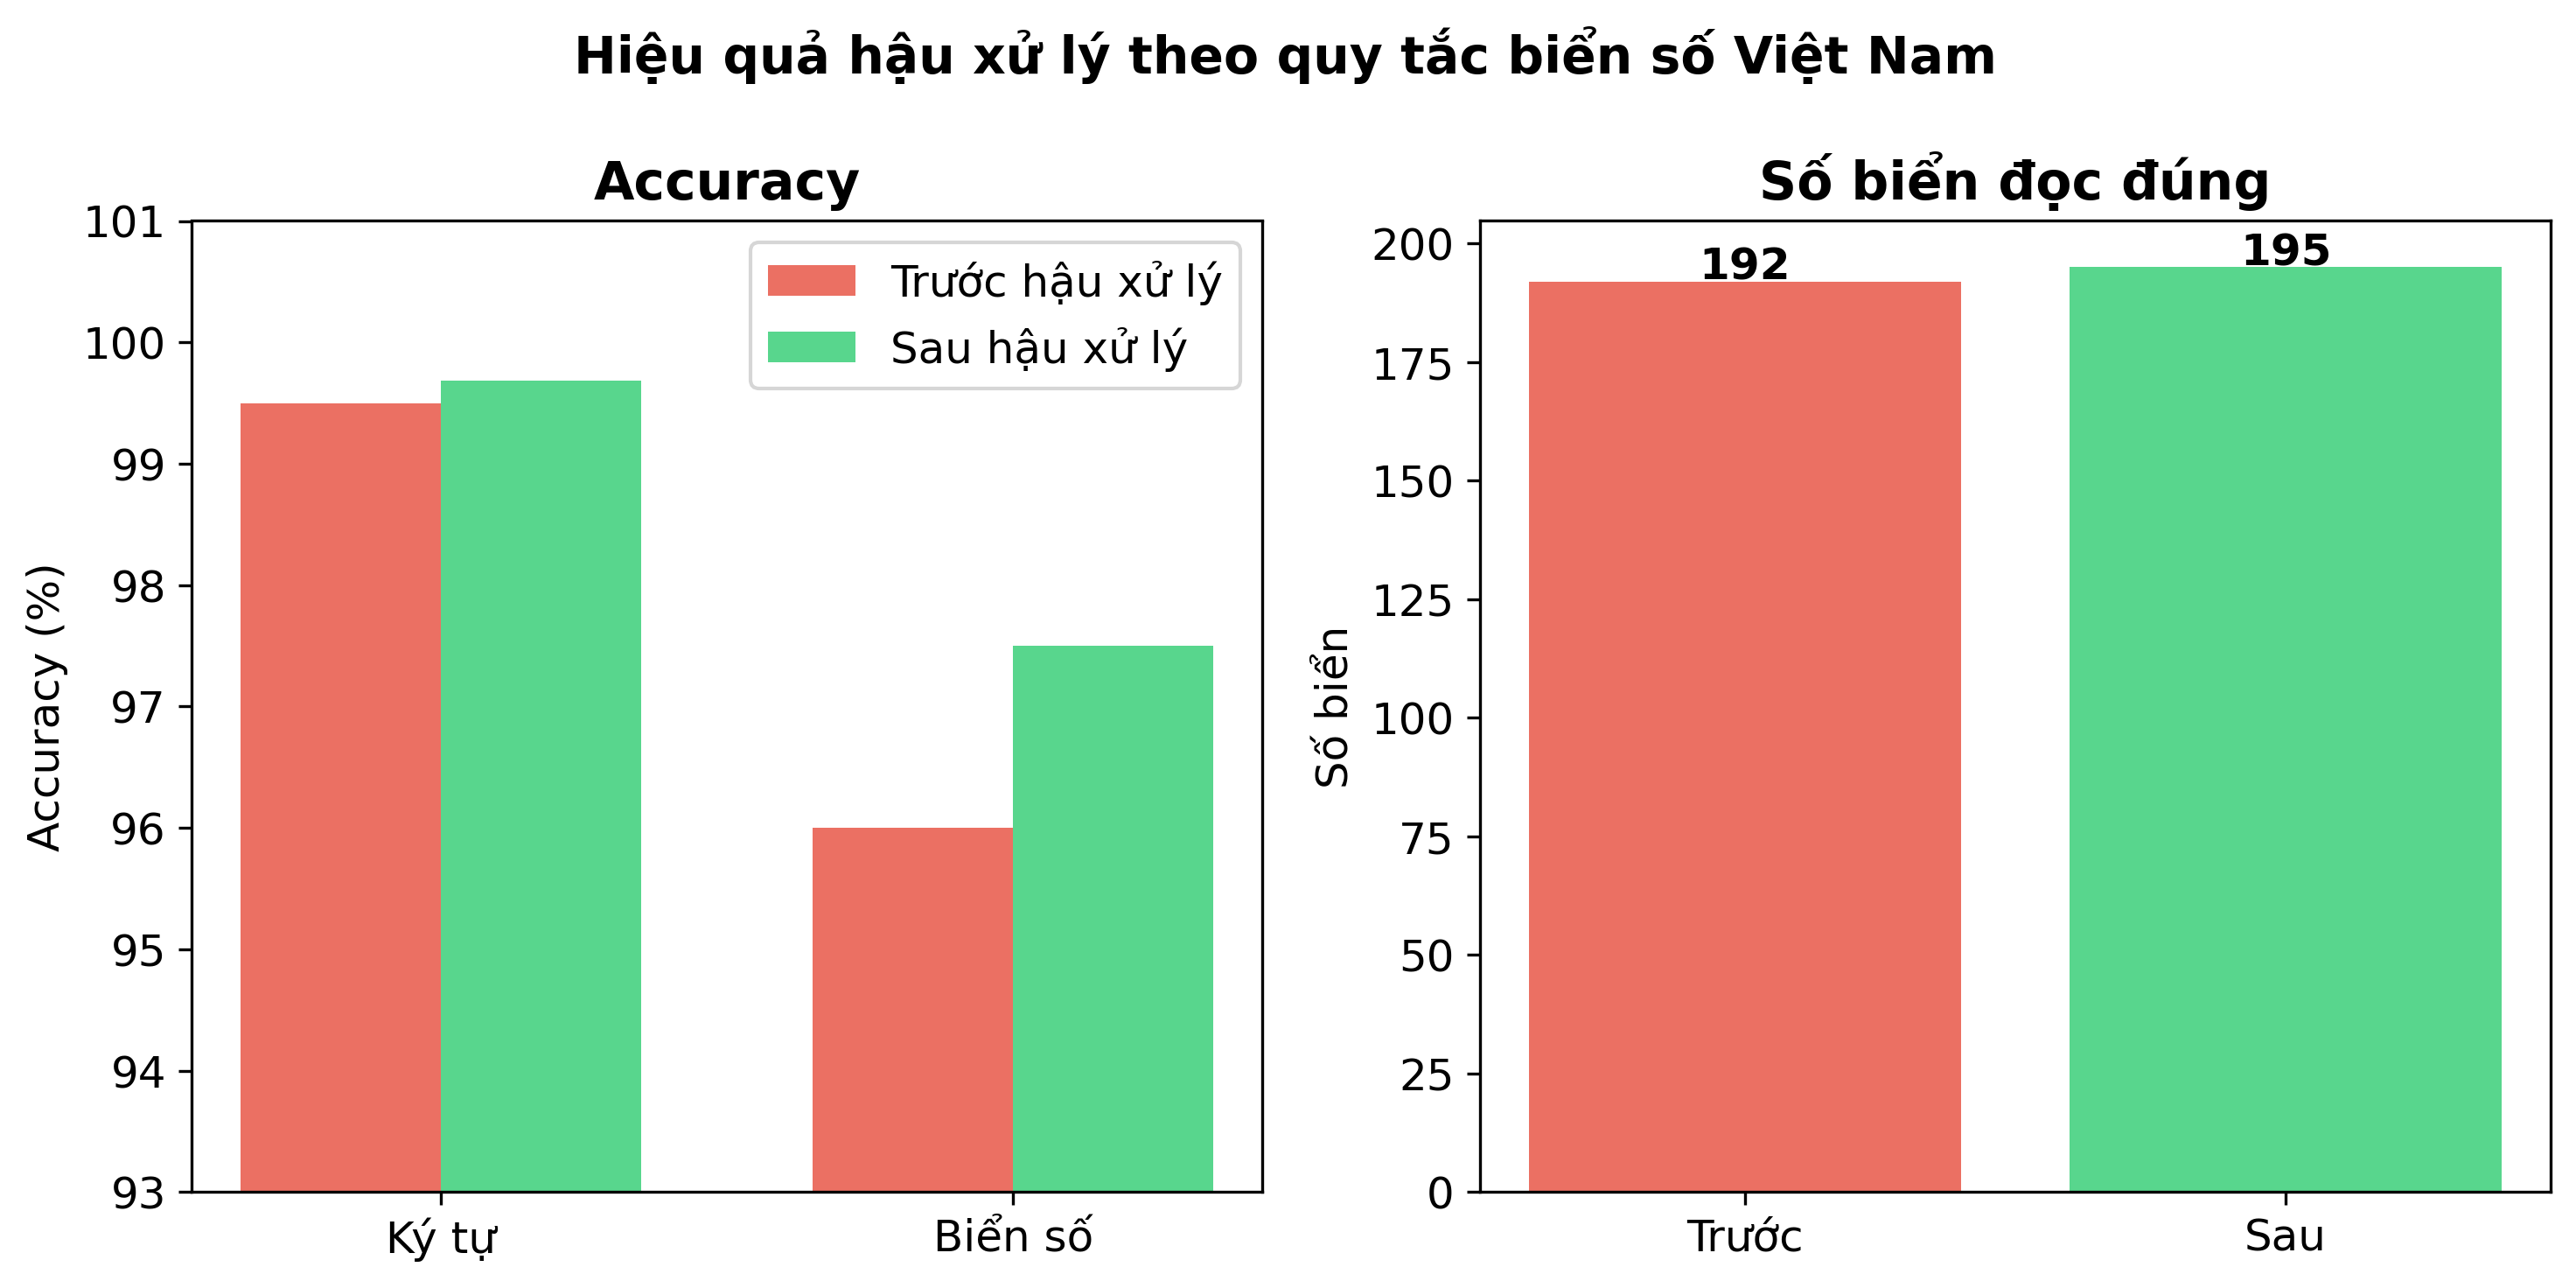
\includegraphics[width=0.85\textwidth]{so_sanh_hau_xu_ly.png}
\caption{Biểu đồ so sánh trước và sau hậu xử lý}
\label{fig:ss_hau_xu_ly}
\end{figure}

\subsection{Báo cáo phân lớp theo từng ký tự}

Đánh giá chi tiết khả năng nhận diện từng ký tự trên tập test 200 ảnh (tổng 1600 ký tự):

\begin{table}[H]
\centering
\caption{Báo cáo phân lớp chi tiết OCR theo từng ký tự}
\label{tab:classification}
\begin{tabular}{crrrr}
\toprule
\textbf{Ký tự} & \textbf{Precision} & \textbf{Recall} & \textbf{F1-Score} & \textbf{Số mẫu} \\
\midrule
0 & 1.00 & 1.00 & 1.00 & 123 \\
1 & 1.00 & 1.00 & 1.00 & 326 \\
2 & 0.98 & 0.99 & 0.99 & 126 \\
3 & 1.00 & 0.99 & 0.99 & 82 \\
4 & 1.00 & 1.00 & 1.00 & 87 \\
5 & 1.00 & 1.00 & 1.00 & 270 \\
6 & 0.99 & 0.99 & 0.99 & 121 \\
7 & 1.00 & 1.00 & 1.00 & 87 \\
8 & 1.00 & 1.00 & 1.00 & 92 \\
9 & 0.99 & 1.00 & 0.99 & 86 \\
A & 1.00 & 1.00 & 1.00 & 55 \\
B & 1.00 & 1.00 & 1.00 & 1 \\
D & 1.00 & 1.00 & 1.00 & 1 \\
E & 1.00 & 1.00 & 1.00 & 1 \\
F & 1.00 & 1.00 & 1.00 & 86 \\
G & 1.00 & 1.00 & 1.00 & 56 \\
\midrule
\textbf{Weighted avg} & \textbf{1.00} & \textbf{1.00} & \textbf{1.00} & \textbf{1600} \\
\bottomrule
\end{tabular}
\end{table}

Nhận xét:
\begin{itemize}[leftmargin=2em]
  \item Accuracy tổng $\sim$100\% trên tập 1600 ký tự (sau hậu xử lý).
  \item Ký tự dễ nhầm nhất: \textbf{2} (precision 0.98), \textbf{6} và \textbf{9} (precision 0.99).
  \item Ký tự \textbf{1} và \textbf{5} có số mẫu lớn nhất (326 và 270).
\end{itemize}

\subsection{Phân bố ký tự trong tập đánh giá}

\begin{figure}[H]
\centering
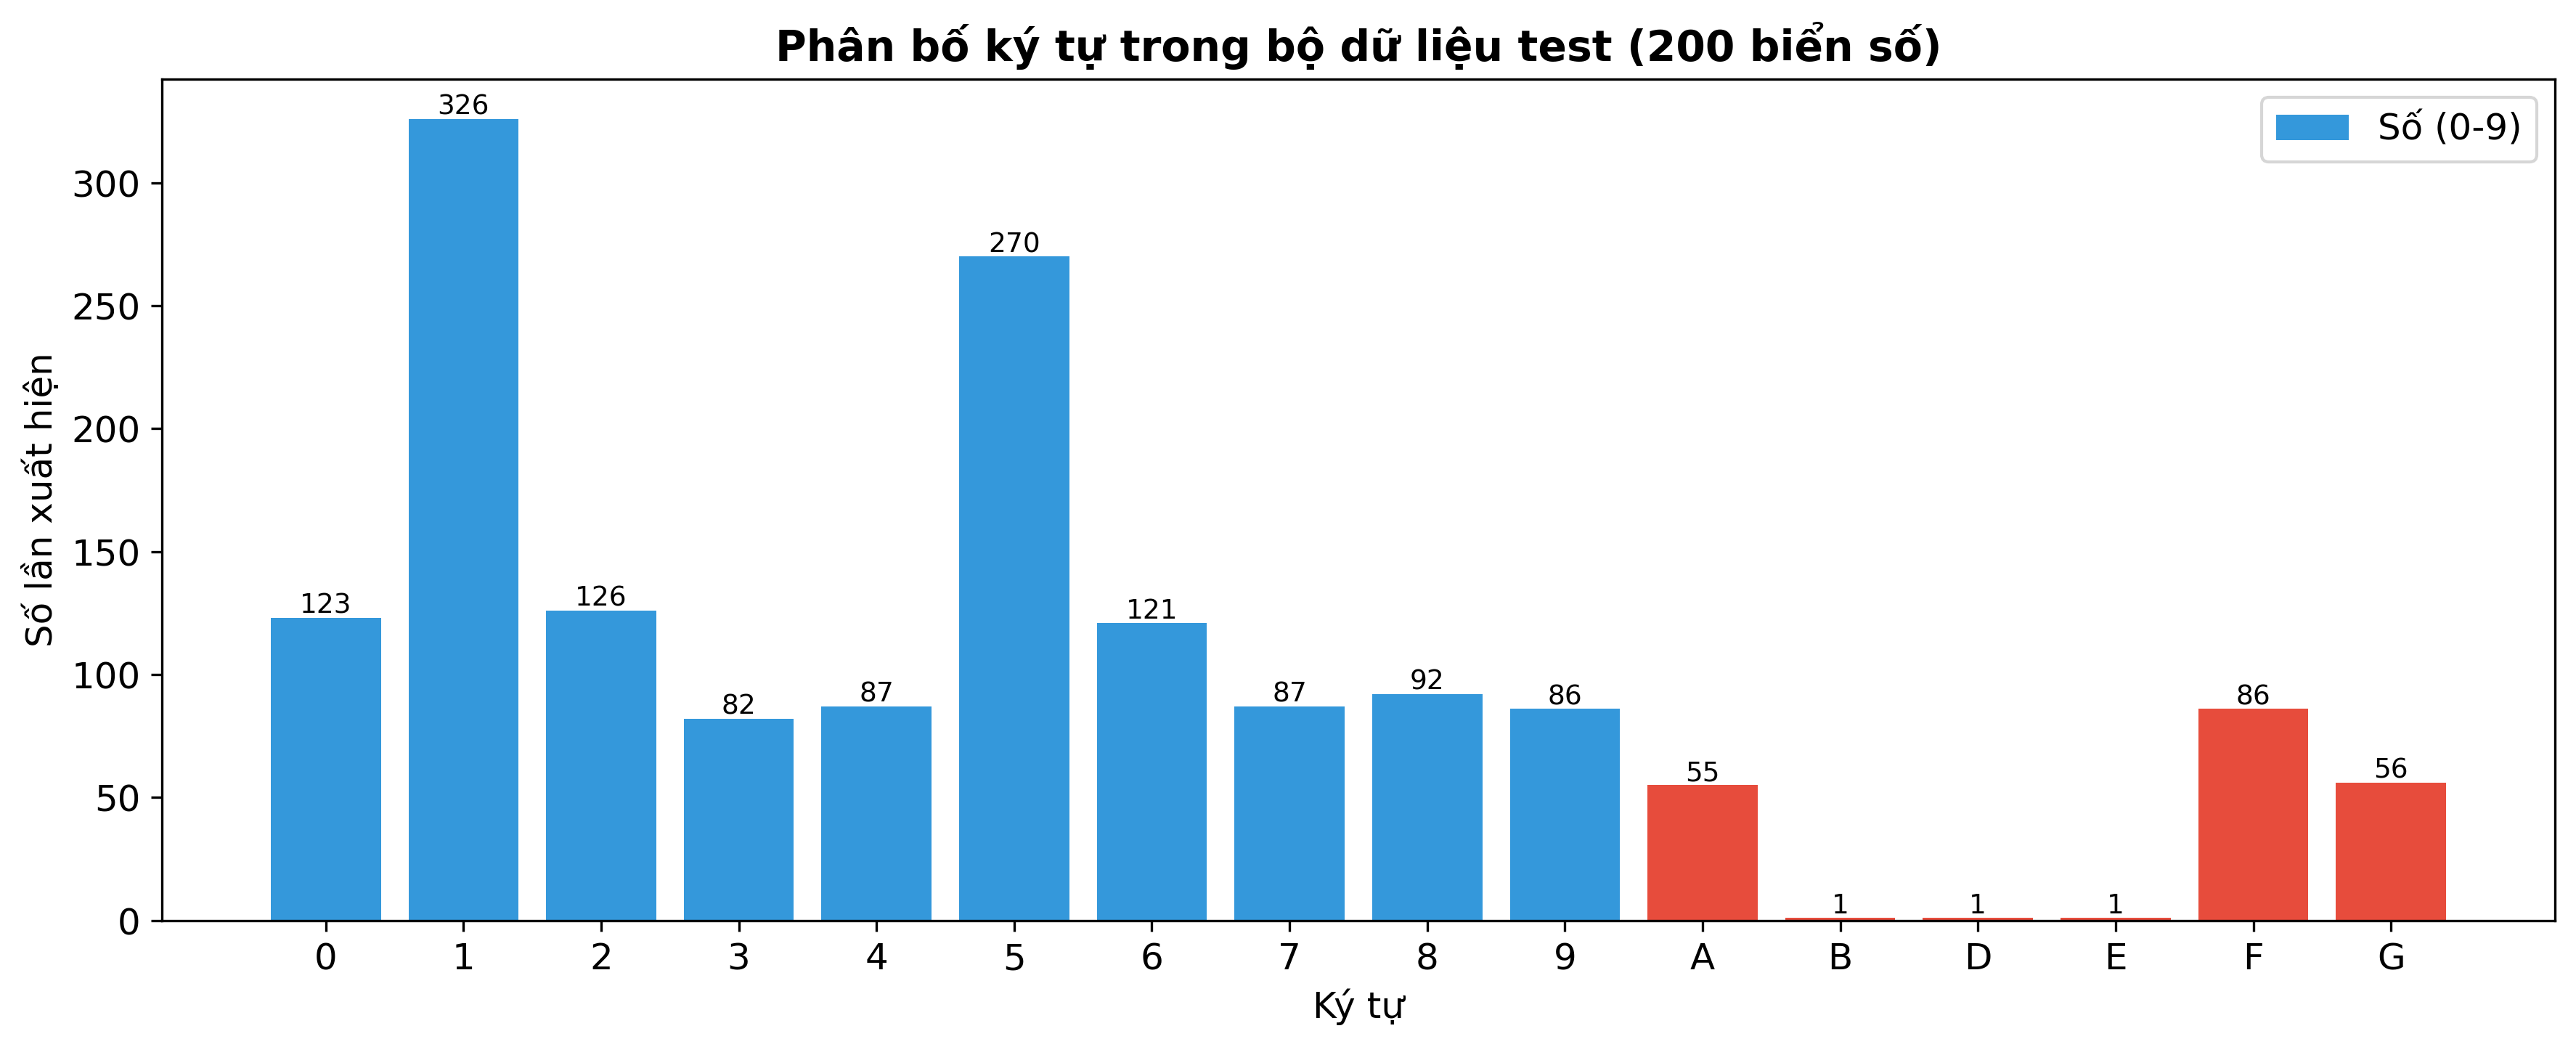
\includegraphics[width=0.85\textwidth]{phan_bo_ky_tu.png}
\caption{Phân bố ký tự trong tập đánh giá OCR}
\label{fig:phan_bo_kt}
\end{figure}

\subsection{Ma trận nhầm lẫn OCR}

\begin{figure}[H]
\centering
\begin{subfigure}[b]{0.48\textwidth}
  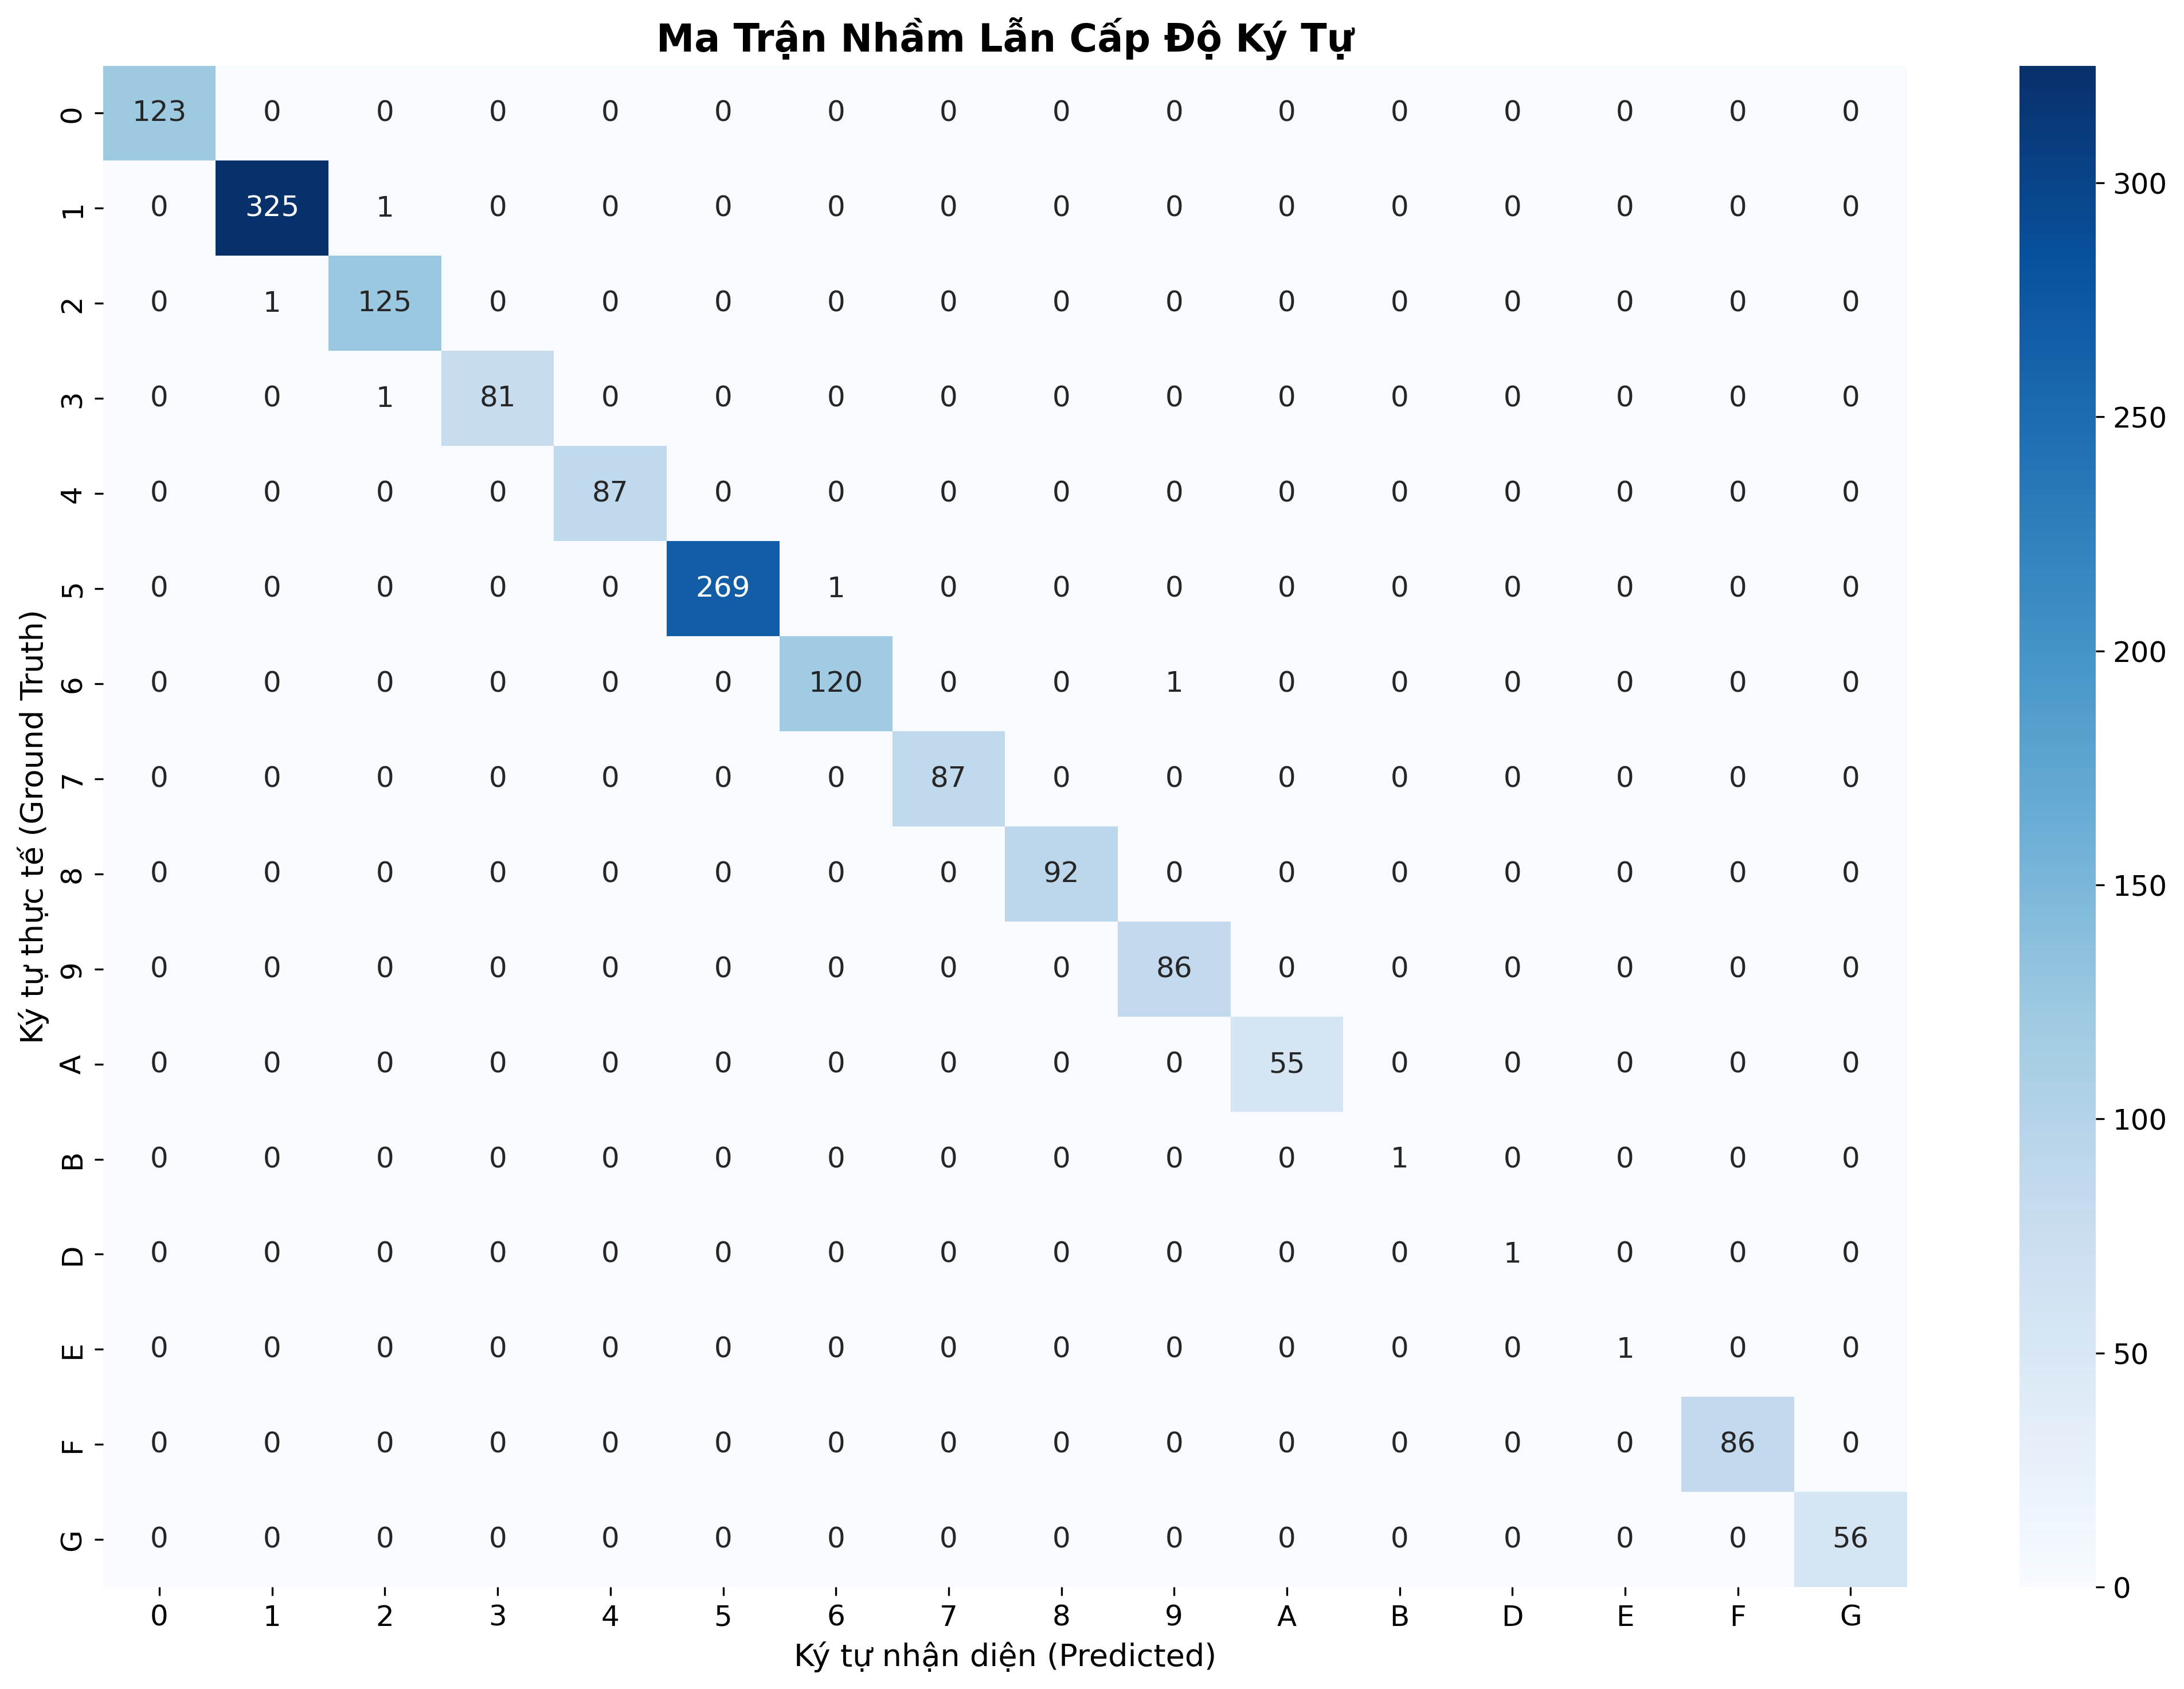
\includegraphics[width=0.85\textwidth]{confusion_matrix_kytu.png}
  \caption{Ma trận nhầm lẫn theo ký tự}
\end{subfigure}
\hfill
\begin{subfigure}[b]{0.48\textwidth}
  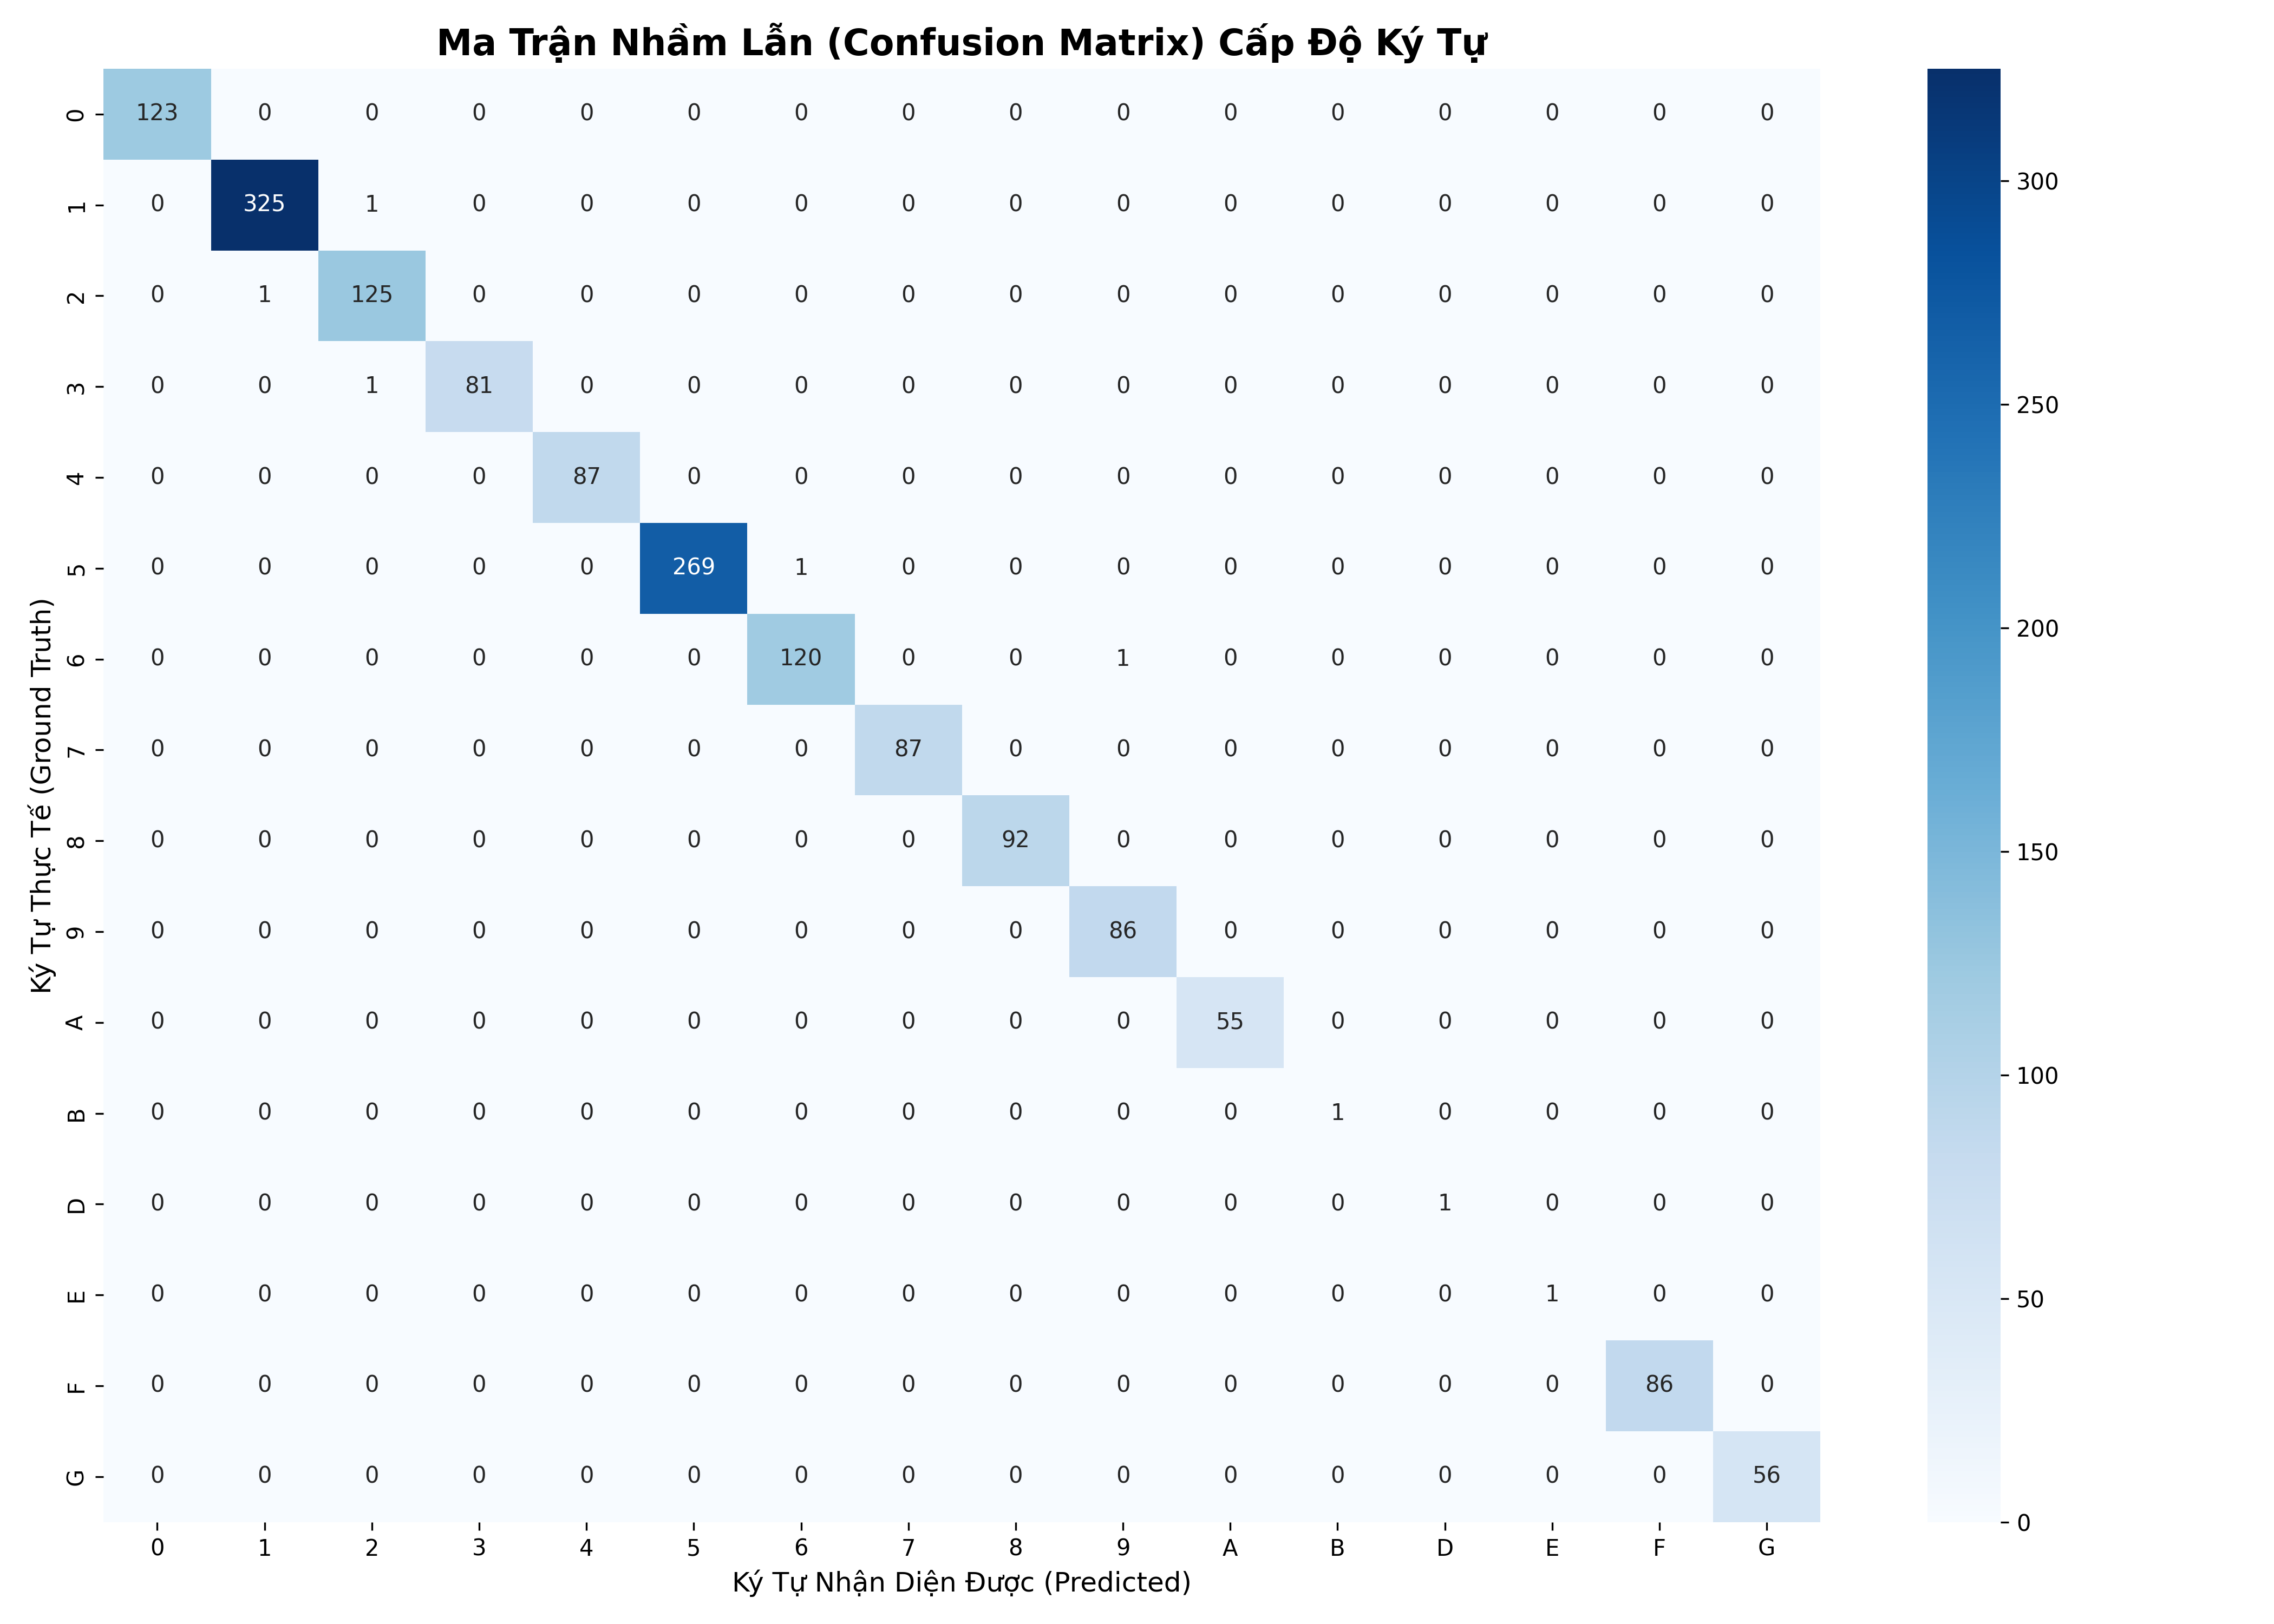
\includegraphics[width=0.85\textwidth]{confusion_matrix_ocr.png}
  \caption{Ma trận nhầm lẫn tổng hợp}
\end{subfigure}
\caption{Ma trận nhầm lẫn OCR}
\label{fig:cm_ocr}
\end{figure}

Ma trận nhầm lẫn OCR cho thấy đường chéo chính rất đậm (hầu hết ký tự được nhận diện đúng). Một số trường hợp nhầm nhẹ giữa các cặp: 2$\leftrightarrow$Z, 6$\leftrightarrow$G, 0$\leftrightarrow$O, 1$\leftrightarrow$I, 5$\leftrightarrow$S — đây là nhầm lẫn cổ điển mà bước hậu xử lý đã sửa được phần lớn.

\subsection{Ví dụ nhận diện biển số}

\begin{figure}[H]
\centering
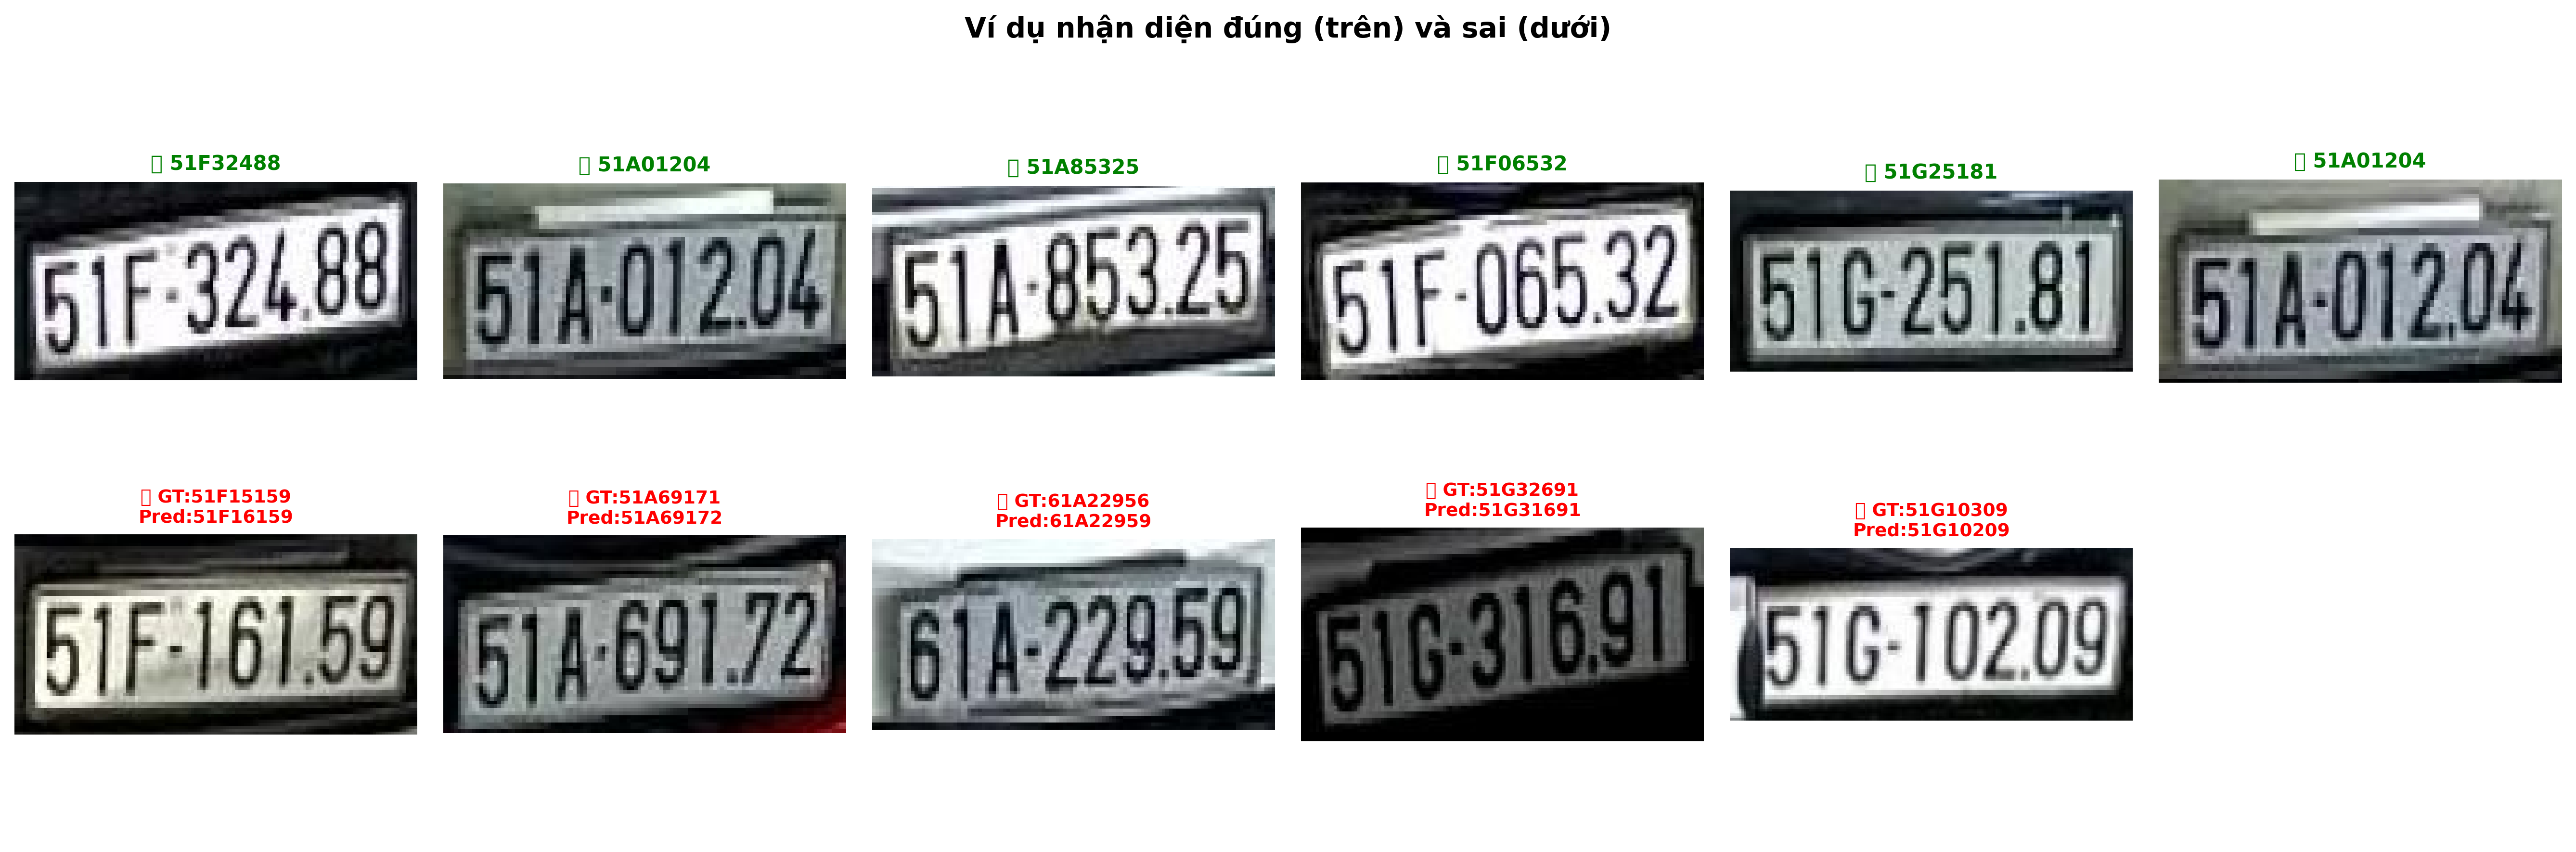
\includegraphics[width=0.85\textwidth]{vi_du_nhan_dien.png}
\caption{Ví dụ nhận diện biển số trên tập test}
\label{fig:vi_du}
\end{figure}

\section{Thiết kế luồng xe vào}

\textbf{Hình 3.3} mô tả luồng xử lý xe vào theo hướng từ trên xuống. Các nhánh rẽ thể hiện trường hợp từ chối mở cổng khi không đọc được biển số, biển số không hợp lệ, xe đã có trong bãi hoặc bãi đã đầy.

Luồng xe vào được thiết kế như sau:

1. Xe tiến tới cổng vào.
2. Cảm biến cổng vào phát hiện vật cản.
3. Arduino (bo mạch vi điều khiển) gửi trạng thái cảm biến về máy tính.
4. Bộ điều khiển lấy ảnh mới nhất từ camera (thiết bị thu hình) vào.
5. Khối AI (trí tuệ nhân tạo) nhận diện biển số.
6. Bộ điều khiển kiểm tra các điều kiện:
\begin{itemize}[leftmargin=2em]
  \item Biển số có đọc được hay không.
  \item Biển số có nằm trong danh sách hợp lệ hay không.
  \item Xe đã có trong bãi hay chưa.
  \item Bãi còn chỗ trống hay không.
\end{itemize}
7. Nếu hợp lệ, hệ thống ghi xe vào cơ sở dữ liệu.
8. Bộ điều khiển gửi lệnh mở barrier (thanh chắn/barie) vào.
9. Khi xe đi qua và cảm biến không còn phát hiện vật cản, hệ thống chờ 2 giây.
10. Bộ điều khiển gửi lệnh đóng barrier (thanh chắn/barie) vào.

Nếu một trong các điều kiện kiểm tra không đạt, hệ thống không mở barrier (thanh chắn/barie) và ghi thông báo vào nhật ký.

\begin{figure}[H]
\centering
\begin{tikzpicture}[node distance=0.8cm, every node/.style={font=\small}]
  \node[block] (a) {Xe tiến tới cổng vào};
  \node[block, below=of a] (b) {Cảm biến phát hiện xe};
  \node[block, below=of b] (c) {AI nhận diện biển số};
  \node[decision, below=0.8cm of c] (d) {Đọc được\\biển số?};
  \node[reject, right=2cm of d] (d_no) {Thử lại};
  \node[decision, below=1cm of d] (e) {Biển số\\hợp lệ?};
  \node[reject, right=2cm of e] (e_no) {Từ chối};
  \node[decision, below=1cm of e] (f) {Xe đã\\trong bãi?};
  \node[reject, right=2cm of f] (f_yes) {Đã có};
  \node[decision, below=1cm of f] (g) {Bãi còn\\chỗ?};
  \node[reject, right=2cm of g] (g_no) {Bãi đầy};
  \node[accept, below=1cm of g] (h) {Ghi xe vào DB\\Mở barrier};
  \node[block, below=of h] (i) {Chờ xe qua + 2s};
  \node[block, fill=red!10, below=of i] (j) {Đóng barrier};
  
  \draw[arrow] (a) -- (b);
  \draw[arrow] (b) -- (c);
  \draw[arrow] (c) -- (d);
  \draw[arrow] (d) -- node[above]{Không} (d_no);
  \draw[arrow] (d) -- node[left]{Có} (e);
  \draw[arrow] (e) -- node[above]{Không} (e_no);
  \draw[arrow] (e) -- node[left]{Có} (f);
  \draw[arrow] (f) -- node[above]{Có} (f_yes);
  \draw[arrow] (f) -- node[left]{Không} (g);
  \draw[arrow] (g) -- node[above]{Không} (g_no);
  \draw[arrow] (g) -- node[left]{Có} (h);
  \draw[arrow] (h) -- (i);
  \draw[arrow] (i) -- (j);
\end{tikzpicture}
\caption{Lưu đồ xử lý xe vào}
\label{fig:xe_vao}
\end{figure}

\section{Thiết kế luồng xe ra}

\textbf{Hình 3.4} mô tả luồng xử lý xe ra. Điểm khác biệt quan trọng là dữ liệu xe chỉ được xóa khỏi bảng xe trong bãi sau khi xe đã đi qua, cảm biến quang và barrier (thanh chắn/barie) đã đóng lại.

Luồng xe ra được thiết kế theo hướng chặt chẽ hơn so với việc chỉ giảm số lượng xe tự động. Hệ thống cần xác định biển số xe ra và kiểm tra xe đó có đang ở trong bãi hay không.

Các bước xử lý:

1. Xe tiến tới cổng ra.
2. Cảm biến cổng ra phát hiện vật cản.
3. Arduino (bo mạch vi điều khiển) gửi trạng thái cảm biến về máy tính.
4. Bộ điều khiển lấy ảnh từ camera (thiết bị thu hình) ra.
5. Khối AI (trí tuệ nhân tạo) nhận diện biển số xe ra.
6. Bộ điều khiển kiểm tra biển số có tồn tại trong danh sách xe đang ở trong bãi không.
7. Nếu có, hệ thống mở barrier (thanh chắn/barie) ra.
8. Xe đi qua cổng ra.
9. Khi cảm biến không còn phát hiện vật cản, hệ thống chờ 2 giây.
10. Bộ điều khiển đóng barrier (thanh chắn/barie) ra.
11. Sau khi đóng barrier (thanh chắn/barie), hệ thống mới xóa biển số khỏi danh sách xe trong bãi và ghi lịch sử ra.

Cách thiết kế này tránh lỗi xóa xe khỏi bãi quá sớm. Nếu barrier (thanh chắn/barie) mở nhưng xe chưa đi qua, dữ liệu vẫn chưa bị cập nhật sai.

\begin{figure}[H]
\centering
\begin{tikzpicture}[node distance=0.8cm, every node/.style={font=\small}]
  \node[block] (a) {Xe tiến tới cổng ra};
  \node[block, below=of a] (b) {Cảm biến phát hiện xe};
  \node[block, below=of b] (c) {AI nhận diện biển số};
  \node[decision, below=0.8cm of c] (d) {Đọc được\\biển số?};
  \node[reject, right=2cm of d] (d_no) {Thử lại};
  \node[decision, below=1cm of d] (e) {Xe có\\trong bãi?};
  \node[reject, right=2cm of e] (e_no) {Không có};
  \node[accept, below=1cm of e] (f) {Mở barrier ra};
  \node[block, below=of f] (g) {Chờ xe qua + 2s};
  \node[block, fill=red!10, below=of g] (h) {Đóng barrier};
  \node[block, fill=blue!10, below=of h] (i) {Xóa xe khỏi DB\\Ghi lịch sử RA};
  
  \draw[arrow] (a) -- (b);
  \draw[arrow] (b) -- (c);
  \draw[arrow] (c) -- (d);
  \draw[arrow] (d) -- node[above]{Không} (d_no);
  \draw[arrow] (d) -- node[left]{Có} (e);
  \draw[arrow] (e) -- node[above]{Không} (e_no);
  \draw[arrow] (e) -- node[left]{Có} (f);
  \draw[arrow] (f) -- (g);
  \draw[arrow] (g) -- (h);
  \draw[arrow] (h) -- (i);
\end{tikzpicture}
\caption{Lưu đồ xử lý xe ra}
\label{fig:xe_ra}
\end{figure}

\section{Thiết kế khối cơ sở dữ liệu}

Cơ sở dữ liệu gồm bốn bảng chính, được mô tả trong Bảng 3.2.

\textbf{Bảng 3.2. Thiết kế các bảng dữ liệu chính}

Các thao tác chính với cơ sở dữ liệu:

\begin{itemize}[leftmargin=2em]
  \item Thêm biển số hợp lệ.
  \item Xóa biển số hợp lệ.
  \item Kiểm tra biển số có hợp lệ không.
  \item Thêm xe vào danh sách xe trong bãi.
  \item Kiểm tra xe có đang trong bãi không.
  \item Xóa xe khỏi bãi khi xe ra.
  \item Đếm số xe hiện tại.
  \item Lấy lịch sử vào ra.
\end{itemize}
Trong hệ thống, dữ liệu xe trong bãi có vai trò quyết định. Xe chỉ được ra khi biển số được nhận diện tại cổng ra tồn tại trong bảng xe đang ở trong bãi.

\begin{table}[H]
\centering
\caption{Thiết kế các bảng dữ liệu chính}
\label{tab:bang_dl}
\begin{tabular}{ll}
\toprule
\textbf{Bảng} & \textbf{Chức năng} \\
\midrule
\texttt{cai\_dat} & Lưu cấu hình hệ thống (sức chứa bãi xe) \\
\texttt{bien\_so\_hop\_le} & Lưu danh sách biển số được phép vào \\
\texttt{xe\_trong\_bai} & Lưu các xe đang có trong bãi \\
\texttt{lich\_su\_ra\_vao} & Lưu lịch sử xe vào và xe ra \\
\bottomrule
\end{tabular}
\end{table}

\section{Thiết kế khối phần cứng barrier}

Khối phần cứng gồm:

\begin{itemize}[leftmargin=2em]
  \item Arduino (bo mạch vi điều khiển).
  \item Hai servo (động cơ điều khiển theo góc quay): một cho cổng vào, một cho cổng ra.
  \item Hai cảm biến LM393 (module cảm biến vật cản dùng IC so sánh LM393): một ở cổng vào, một ở cổng ra.
  \item Nguồn cấp cho Arduino (bo mạch vi điều khiển) và servo (động cơ điều khiển theo góc quay).
  \item Kết nối USB (Universal Serial Bus - chuẩn kết nối giữa máy tính và thiết bị) giữa Arduino (bo mạch vi điều khiển) và máy tính.
\end{itemize}
\textbf{Hình 3.5} mô tả sơ đồ đấu nối phần cứng. Các mũi tên từ Arduino (bo mạch vi điều khiển) đến servo (động cơ điều khiển theo góc quay) là tín hiệu điều khiển PWM (Pulse Width Modulation - điều chế độ rộng xung) một chiều: Arduino phát xung điều khiển góc quay cho servo. Các mũi tên từ cảm biến LM393 (module cảm biến vật cản dùng IC so sánh LM393) về Arduino là tín hiệu số một chiều: cảm biến xuất mức logic tại chân DO (Digital Output - ngõ ra số), Arduino đọc tại các chân digital (chân số). Mũi tên giữa máy tính và Arduino là giao tiếp Serial (giao tiếp nối tiếp) hai chiều qua USB (chuẩn kết nối giữa máy tính và thiết bị): máy tính gửi lệnh, Arduino gửi trạng thái cảm biến và phản hồi.

Trong mô hình, servo (động cơ điều khiển theo góc quay) cổng vào nối chân tín hiệu với D9, servo cổng ra nối chân tín hiệu với D10. Cảm biến LM393 (module cảm biến vật cản dùng IC so sánh LM393) cổng vào nối DO (Digital Output - ngõ ra số) với D2, cảm biến LM393 cổng ra nối DO với D3. Hai cảm biến được cấp VCC (Voltage Common Collector - chân cấp nguồn dương) và GND (Ground - chân mass/đất chung) từ Arduino (bo mạch vi điều khiển). Nếu servo dùng nguồn 5V ngoài để tránh sụt áp, bắt buộc GND của nguồn servo phải nối chung với GND Arduino; nếu không, tín hiệu điều khiển từ Arduino sang servo sẽ không có cùng mốc điện áp và servo có thể rung hoặc không hoạt động đúng.

Nguyên lý hoạt động của phần cứng:

1. Arduino (bo mạch vi điều khiển) đọc trạng thái cảm biến theo chu kỳ.
2. Khi trạng thái cảm biến thay đổi hoặc đến chu kỳ gửi trạng thái, Arduino (bo mạch vi điều khiển) gửi dữ liệu lên máy tính.
3. Khi nhận lệnh mở hoặc đóng, Arduino điều khiển servo (động cơ điều khiển theo góc quay) quay đến góc tương ứng.
4. Servo (động cơ điều khiển theo góc quay) được điều khiển từng bước nhỏ để chuyển động mượt hơn.

Một số lưu ý khi lắp đặt phần cứng:

\begin{itemize}[leftmargin=2em]
  \item Cảm biến LM393 (module cảm biến vật cản dùng IC so sánh LM393) cần được chỉnh biến trở để khoảng cách phát hiện phù hợp với kích thước mô hình.
  \item Vùng phát hiện của cảm biến nên đặt đúng vị trí xe đi qua barrier (thanh chắn/barie), không đặt quá xa khiến barrier đóng sai thời điểm.
  \item Servo SG90 (động cơ servo cỡ nhỏ SG90) có dòng khởi động tương đối lớn, nếu dùng nguồn USB (chuẩn kết nối giữa máy tính và thiết bị) yếu có thể làm Arduino (bo mạch vi điều khiển) reset hoặc servo giật.
  \item Dây tín hiệu servo nên cắm đúng chân điều khiển, dây đỏ là VCC (chân cấp nguồn dương), dây nâu/đen là GND (mass/đất chung), dây cam/vàng là tín hiệu.
  \item Khi thử phần cứng, nên dùng lệnh \texttt{SERVO\_TEST} trước để kiểm tra hai servo (động cơ điều khiển theo góc quay) độc lập với giao diện.
  \item Barrier (thanh chắn/barie) cơ khí cần nhẹ và không kẹt trục để servo (động cơ điều khiển theo góc quay) không quá tải.
\end{itemize}

\begin{figure}[H]
\centering
\begin{tikzpicture}[node distance=1.2cm, every node/.style={font=\small}]
  \node[block, fill=gray!20, minimum width=4cm] (pc) {Máy tính\\Python Software};
  \node[block, fill=blue!15, minimum width=4cm, below=1.5cm of pc] (ard) {Arduino Uno};
  
  \node[block, fill=green!15, below left=2cm and 1cm of ard] (sv1) {Servo cổng VÀO\\(D9 - PWM)};
  \node[block, fill=green!15, below right=2cm and 1cm of ard] (sv2) {Servo cổng RA\\(D10 - PWM)};
  \node[block, fill=yellow!15, left=2cm of ard] (cb1) {LM393 cổng VÀO\\(D2 - Digital)};
  \node[block, fill=yellow!15, right=2cm of ard] (cb2) {LM393 cổng RA\\(D3 - Digital)};
  
  \draw[darrow] (pc) -- node[right, font=\scriptsize, align=center, text width=1.5cm]{USB Serial 9600 baud} (ard);
  \draw[arrow] (ard) -- node[left, font=\scriptsize]{PWM} (sv1);
  \draw[arrow] (ard) -- node[right, font=\scriptsize]{PWM} (sv2);
  \draw[arrow] (cb1) -- node[above, font=\scriptsize]{DO} (ard);
  \draw[arrow] (cb2) -- node[above, font=\scriptsize]{DO} (ard);
\end{tikzpicture}
\caption{Sơ đồ đấu nối phần cứng Arduino -- Servo -- Cảm biến}
\label{fig:phan_cung}
\end{figure}

\section{Đánh giá chức năng điều khiển barrier}

Khối điều khiển barrier (thanh chắn/barie) hoạt động theo đúng nguyên tắc:

\begin{itemize}[leftmargin=2em]
  \item Khi có lệnh mở, servo (động cơ điều khiển theo góc quay) nâng barrier (thanh chắn/barie) lên.
  \item Khi xe đi qua, cảm biến chuyển từ trạng thái có vật cản sang không có vật cản.
  \item Hệ thống chờ 2 giây sau khi cảm biến không còn phát hiện vật cản.
  \item Sau thời gian chờ, Arduino (bo mạch vi điều khiển) nhận lệnh đóng barrier (thanh chắn/barie).
\end{itemize}
Việc điều khiển servo (động cơ điều khiển theo góc quay) theo từng bước nhỏ giúp chuyển động barrier (thanh chắn/barie) mềm hơn so với việc quay ngay lập tức đến góc đích. Cơ chế chờ sau khi cảm biến hết vật cản giúp mô hình vận hành sát thực tế hơn.

\section{Thiết kế đa luồng}

\textbf{Hình 3.6} mô tả cách tách các tác vụ có thời gian xử lý khác nhau ra nhiều luồng. Camera (thiết bị thu hình), AI (trí tuệ nhân tạo) và cảm biến chạy tách khỏi luồng giao diện để giao diện không bị treo khi nhận diện hoặc đọc thiết bị.

Hệ thống có nhiều tác vụ diễn ra đồng thời:

\begin{itemize}[leftmargin=2em]
  \item Đọc camera (thiết bị thu hình) liên tục.
  \item Chạy AI (trí tuệ nhân tạo) nhận diện biển số.
  \item Đọc trạng thái cảm biến từ Arduino (bo mạch vi điều khiển).
  \item Cập nhật giao diện.
  \item Truy vấn cơ sở dữ liệu.
\end{itemize}
Nếu tất cả tác vụ chạy trên cùng một luồng, giao diện có thể bị treo khi AI (trí tuệ nhân tạo) xử lý lâu hoặc khi camera (thiết bị thu hình) chậm phản hồi. Vì vậy hệ thống sử dụng cách tổ chức đa luồng: camera, AI và cảm biến được xử lý tách khỏi luồng giao diện. Giao diện chỉ lấy trạng thái mới nhất để hiển thị định kỳ.

---

\begin{figure}[H]
\centering
\begin{tikzpicture}[node distance=0.8cm, every node/.style={font=\small}]
  \node[block, fill=cyan!20] (main) {Luồng chính (UI)\\Tkinter mainloop\\poll() mỗi 50ms};
  
  \node[block, fill=green!15, minimum width=3cm, above left=1.5cm and 0.5cm of main] (cam1) {Luồng Camera vào\\Đọc frame liên tục};
  \node[block, fill=green!15, minimum width=3cm, above right=1.5cm and 0.5cm of main] (cam2) {Luồng Camera ra\\Đọc frame liên tục};
  \node[block, fill=purple!15, minimum width=3cm, below left=1.5cm and 0.5cm of main] (ai) {Luồng AI\\YOLO + OCR};
  \node[block, fill=yellow!15, minimum width=3cm, below right=1.5cm and 0.5cm of main] (sen) {Luồng Cảm biến\\Đọc Serial 100ms};
  
  \draw[arrow] (cam1) -- node[left, font=\scriptsize]{latest\_frame} (main);
  \draw[arrow] (cam2) -- node[right, font=\scriptsize]{latest\_frame} (main);
  \draw[arrow] (ai) -- node[left, font=\scriptsize]{q\_msg} (main);
  \draw[arrow] (sen) -- node[right, font=\scriptsize]{q\_sensor} (main);
  \draw[arrow] (main) -- node[right, font=\scriptsize]{q\_ai} (ai);
\end{tikzpicture}
\caption{Cơ chế đa luồng trong hệ thống}
\label{fig:da_luong}
\end{figure}

\section{Kết quả giao diện và vận hành}

Giao diện hệ thống hiển thị được các thành phần chính:

\begin{itemize}[leftmargin=2em]
  \item Hình ảnh camera (thiết bị thu hình) cổng vào.
  \item Hình ảnh camera (thiết bị thu hình) cổng ra.
  \item Ảnh biển số sau xử lý của từng cổng.
  \item Chuỗi biển số nhận diện được.
  \item Số lượng xe hiện tại và sức chứa bãi.
  \item Chế độ thủ công/tự động.
  \item Trạng thái kết nối Arduino (bo mạch vi điều khiển).
  \item Danh sách biển số hợp lệ.
  \item Nhật ký sự kiện.
\end{itemize}
Trong quá trình thử nghiệm, hệ thống thực hiện được các chức năng:

\begin{itemize}[leftmargin=2em]
  \item Bật và tắt từng camera (thiết bị thu hình).
  \item Chuyển camera (thiết bị thu hình) cho từng cổng.
  \item Nhận diện biển số ở cổng vào.
  \item Nhận diện biển số ở cổng ra.
  \item Thêm và xóa biển số hợp lệ.
  \item Tự động mở barrier (thanh chắn/barie) khi xe đủ điều kiện.
  \item Không mở barrier (thanh chắn/barie) khi biển số không hợp lệ.
  \item Không cho xe vào khi bãi đã đầy.
  \item Không cho xe ra nếu xe không có trong bãi.
  \item Đóng barrier (thanh chắn/barie) sau khi cảm biến không còn phát hiện vật cản trong 2 giây.
\end{itemize}

\section{Đánh giá ưu điểm}

Hệ thống đạt được các ưu điểm chính:

\begin{itemize}[leftmargin=2em]
  \item Có đủ hai luồng cổng vào và cổng ra.
  \item Mỗi cổng có camera (thiết bị thu hình) và vùng hiển thị biển số riêng.
  \item Có kiểm tra biển số hợp lệ trước khi cho xe vào.
  \item Có kiểm tra xe trong bãi trước khi cho xe ra.
  \item Không xóa xe khỏi bãi trước khi xe thật sự ra khỏi vùng cổng.
  \item Có chế độ tự động và thủ công.
  \item Có giao diện trực quan, dễ quan sát trạng thái.
  \item Cơ sở dữ liệu được tổ chức rõ ràng.
  \item Giao tiếp Arduino (bo mạch vi điều khiển) đơn giản, dễ kiểm tra và phân tích lỗi khi ghép nối phần cứng.
  \item Cơ chế đóng barrier (thanh chắn/barie) có xét trạng thái cảm biến, tăng tính an toàn.
\end{itemize}

\section{Hạn chế}

Bên cạnh các kết quả đạt được, hệ thống vẫn còn một số hạn chế:

\begin{itemize}[leftmargin=2em]
  \item Độ chính xác nhận diện phụ thuộc vào góc đặt camera (thiết bị thu hình) và ánh sáng môi trường.
  \item Nếu biển số bị đưa quá sát camera (thiết bị thu hình) hoặc bị cắt mất mép, kết quả nhận diện có thể sai.
  \item Chưa có chức năng lưu ảnh xe vào/ra thành hồ sơ.
  \item Chưa có chức năng tính tiền gửi xe.
  \item Chưa có tài khoản quản trị và phân quyền người dùng.
  \item Mô hình mới dừng ở quy mô đồ án, chưa đánh giá trong môi trường bãi xe thực tế ngoài trời.
\end{itemize}

\section{Hướng phát triển}

Trong tương lai, hệ thống có thể được phát triển theo các hướng sau:

\begin{itemize}[leftmargin=2em]
  \item Bổ sung chức năng tính phí theo thời gian gửi xe.
  \item Lưu ảnh xe vào và ảnh xe ra để đối chiếu.
  \item Thêm chức năng xuất báo cáo lịch sử vào/ra.
  \item Xây dựng giao diện web hoặc ứng dụng quản lý từ xa.
  \item Tối ưu nhận diện trong điều kiện thiếu sáng, ngược sáng hoặc biển số bị nghiêng.
  \item Bổ sung cơ chế cảnh báo khi mất kết nối Arduino (bo mạch vi điều khiển) hoặc camera (thiết bị thu hình).
  \item Cải tiến mô hình phần cứng để barrier (thanh chắn/barie) chắc chắn và ổn định hơn.
\end{itemize}

\section{Kết luận}

Đề tài đã xây dựng được mô hình hệ thống bãi đỗ xe tự động có sự kết hợp giữa xử lý ảnh, trí tuệ nhân tạo, cơ sở dữ liệu, giao diện người dùng và điều khiển phần cứng. Hệ thống có thể nhận diện biển số ở cả cổng vào và cổng ra, kiểm tra dữ liệu trước khi mở barrier (thanh chắn/barie), đồng thời cập nhật trạng thái xe trong bãi sau khi xe ra khỏi cổng.

Kết quả thực nghiệm cho thấy phương pháp kết hợp YOLOv8 (mô hình phát hiện đối tượng phiên bản 8), PaddleOCR (bộ nhận dạng ký tự quang học) và hậu xử lý theo quy tắc biển số Việt Nam đạt độ chính xác tốt trong điều kiện mô hình được căn chỉnh phù hợp. Hệ thống đáp ứng được mục tiêu của đồ án và có thể tiếp tục mở rộng để tiệm cận một hệ thống bãi xe thông minh hoàn chỉnh hơn.

\end{document}
